%Dokumentklasse
\documentclass[a4paper,12pt]{scrreprt}
\usepackage[left= 2.5cm,right = 2cm, bottom = 4 cm]{geometry}
%\usepackage[onehalfspacing]{setspace}
% ============= Packages =============


% Dokumentinformationen
\usepackage[
	pdftitle={Bachelorarbeit},
	pdfsubject={},
	pdfauthor={Santoro Sandro, Brunner Gian},
	pdfkeywords={},	
	%Links nicht einrahmen
	hidelinks]{hyperref}

% Standard Packages
\usepackage[utf8]{inputenc}
\usepackage[ngerman]{babel}
\usepackage[T1]{fontenc}
\usepackage{graphicx}
\graphicspath{{img/}}
\usepackage{lmodern}
\usepackage{color}
\usepackage{siunitx}
\usepackage{tikz}
\usepackage{caption}
\usepackage{placeins}
\usepackage{tabularx}
\usepackage{arydshln}
\usepackage{pdfpages}
\usepackage{listings}
\usepackage{url}
\usepackage{mathtools}
\usepackage{makecell}
\usepackage{multirow}
\usepackage{booktabs}
\usepackage{float}
\usepackage{apacite}

\sisetup{detect-weight=true, detect-family=true}
\newcommand{\source}[1]{\caption*{Source: {#1}} }


% ============= Kopf- und Fußzeile =============

\usepackage[automark,headsepline]{scrlayer-scrpage} %footsepline
\pagestyle{scrheadings}
\automark[chapter]{chapter}
\clearscrheadfoot

\ihead{\headmark}				%Kopfzeile innen mit Kapitel
\chead{}						%Kopfzeile Mitte
\ohead[\pagemark]{\pagemark}	%Kopfzeile aussen mit Seitennummer

%\ifoot{}						%Fußzeile innen
%\cfoot{}						%Fußzeile Mitte
%\ofoot{}						%Fußzeile außen

\renewcommand*\chapterpagestyle{scrheadings}

%============== Abstände von Kopfzeile zu Text überall gleich ============%
\renewcommand*\chapterheadstartvskip{\vspace*{-\topskip}}
\renewcommand*\chapterheadendvskip{%
\vspace*{1\baselineskip plus .1\baselineskip minus .167\baselineskip}}


% zusätzliche Schriftzeichen der American Mathematical Society
\usepackage{amsfonts}
\usepackage{amsmath}
\usepackage[ngerman]{cleveref}

%nicht einrücken nach Absatz
\setlength{\parindent}{0pt}

%============== Package für Dateistruktur-Baum ============%
\usepackage{forest}

% ============= Package Einstellungen & Sonstiges ============= 
%Besondere Trennungen
\hyphenation{De-zi-mal-tren-nung}


%=========== Abbildungen fangen mit 1 an ===========%
\renewcommand*{\thefigure}{\arabic{figure}}

\addto{\captionsngerman}{%
	\renewcommand*{\source}{Quelle: }
}
% ============= Dokumentbeginn =============
\begin{document}
\setcounter{secnumdepth}{5}	%Bis zu welcher Ebene wird nummeriert?
\setcounter{tocdepth}{4}

%Seite ohne Kopf- und Fußzeile sowie Seitenzahl
\thispagestyle{empty}

\renewcommand*\chapterpagestyle{scrheadings}

\includegraphics[scale=0.5]{img/ntb.jpg}

\begin{center}
\vspace*{4 cm}
\textbf{\Huge Bachelorarbeit}
\end{center}

\begin{center}
\vspace*{1.5 cm}
\LARGE{\textsf{Menü-Crawler\\}}
\large{\textsf{Prototyp einer Search Engine zur Suche von Speisen und Menüs in der deutschsprachigen Schweiz\\}}
\end{center}


\begin{center}
\vspace*{2 cm}
\textbf{ Studierende:} {\textbf{Sandro Santoro \& Gian Brunner\\}}
\end{center}

\begin{center}
\vspace*{1 cm}
Abgabedatum: 9. August 2019
\vspace*{1 cm}
\end{center}


\begin{center}
\begin{tabular}{lll}
\textbf{Referent:} & & Prof. Corsin Capol\\
\medskip
\textbf{Korreferent:} & & Lukas Toggenburger\\
\end{tabular}
\end{center}


\pagestyle{scrheadings}
\pagenumbering{Roman}

\addchap{Abstract}
\addsec{Abstract Deutsch}
Die Idee dieser Arbeit ist das Erstellen einer Suchmaschine, über welche sich Restaurant-übergreifend Menüs und Speisen suchen lassen.
Die Grundlage einer solchen Suchmaschine sind die Websites von Restaurants in Kombination mit Informationen wie z.B. dem Standort.
Um einen Datensatz solcher Websites zu erstellen, ist ein Webcrawler implementiert worden.
Im wissenschaftlichen Teil dieser Arbeit wurde anhand dieses Datensatzes ein Gold Standard erstellt.
Dieser dient dazu, die eigentliche Forschungsfrage beantworten zu können, die folgendermassen lautet:\\
\emph{Können Restaurant-Webseiten mit hoher Wahrscheinlichkeit klassifiziert werden, ob sie Menüinformationen beinhalten?}\\
Vorausgesetzt wird ein F1-Score von 0.8 oder höher, um diese Frage mit \glqq Ja\grqq{} beantworten zu können.
Dabei werden zwei verschiedene Ansätze zur Klassifikation angewandt, namentlich das regelbasierte Klassifizieren sowie das Klassifizieren mittels Machine-Learning.
Um diese Ansätze prüfen zu können, werden mehrere Experimente durchgeführt.
Zum Schluss wird erkannt, dass der gewünschte F1-Score mit beiden Ansätzen knapp verfehlt wurde.
Im praktischen Teil wird neben dem Webcrawler eine Webapplikation erarbeitet, welche als Suchmaschine dient und die klassifizierten Daten dem Benutzer darstellt.
\addsec{Abstract English}
The idea of this work is to create a search engine that can be used to search menus and meals restaurant independently.
The basis of such a search engine are the websites of restaurants in combination with information such as, for example, the location.
To create a dataset of such websites, a web crawler has been implemented.
In the scientific part of this work, a gold standard was created based on this dataset.
This serves to answer the actual research question, which is the following: \\
\emph{Can Webpages of restaurants be classified with high chance of success, if they contain menu information?} \\
An F1 score of 0.8 or higher is required to answer this question with \glqq Yes\grqq{}.
Two different approaches are used for classification, in particular rule-based classification and classification with machine learning.
To be able to test these approaches, several experiments are carried out.
Finally, it is recognized that the desired F1 score was missed with both approaches.
In the practical part, in addition to the webcrawler, a web application will be developed which serves as a search engine and displays the classified data to a user.

%\addchap{Danksagung}
Wir bedanken uns herzlich bei unseren Referenten, Corsin Capol und Lukas Toggenburger, dafür, dass sie uns bei dieser Arbeit viele Freiheiten gelassen und uns viele gute Ratschläge gegeben haben.\\
Zudem bedanken wir uns bei Norman Süsstrunk für die Hilfe bei der Erarbeitung des Webcrawlers.
%\newpage

%Inhaltsverzeichnis
\tableofcontents
\clearpage 
\addchap{Glossar}
Crawlen - Die Tätigkeit eines Webcrawlers: Das Aufrufen und Herunterladen von Webseiten\\
OSM - Opensteetmap, eine freie Geodatenbank\\
SDK - Software Development Kit (SDK) Programmierwerkzeug und Bibliothek, welches hilft, eine Software zu entwickeln\\
Seed - Eine Liste bestehend aus Webseiten, welche gecrawlt werden sollen\\
Stormcrawler - SDK zur Entwicklung eines Webcrawlers\\
Webcrawler - Programm zum automatisierten Aufrufen und Speichern einer Webseite\\
Website - Komplette Internetseite (Startseite inkl. allen Subwebsites) z.B. www.menucrawler.ch\\
Webpage - Spezifischer Teil einer Webseite z.B. www.menucrawler.ch/ueber-uns\\
idempotent - Bei gleicher Eingabe erfolgt stets die gleiche Ausgabe, egal wie oft die Aufgabe ausgeführt wird\\
Open-Source - Software, deren Quelltext frei einsehbar und änderbar ist\\
Big Data - Arbeitsumfeld, indem mit sehr vielen Datenpunkten gearbeitet wird\\
Machine-Learning - Maschinelles Lernen, der Computer wird darauf trainiert, eine Aufgabe zu verrichten\\
Pipelining - Das verbinden von mehreren Aufgaben zu einer Gesamtaufgabe\\
Stream - Kontinuierlicher Fluss von Datensätzen\\
URL - Uniform Ressource Locator - Eindeutiger Link zu einer Webpage\\
Blacklisting - Index, der zur Benachteiligung der darin aufgeführten Einträgen führt\\
Whitelisting - Index, der zur Bevorzugung der darin aufgeführten Einträgen führt\\
Labeling - Kategorisieren von Daten\\
JSON - JavaScript Object Notation, ein kompaktes Dateiformat in lesbarer Textform, geeignet für den Datenaustausch zwischen Anwendungen\\
No free lunch - Ein Theorem, welches besagt, dass es kein universelles Verfahren für die Lösung eines ML-Problems gibt\\
N-Gramme - Wörterkette mit Anzahl N Wörtern\\
Features - Merkmale, mit denen ein ML-Algorithmus trainiert werden kann\\
Feature-Extraction - Das Extrahieren von relevanten Features\\
LSA (Latent Sentiment Analysis) - Verfahren zum Auffinden von Schlüsselbegriffen\\
Bigramm - Eine Wörterkette mit Länge zwei\\
Trigramm - Eine Wörterkette mit Länge drei\\
Scores - Die Resultate, in diesem Zusammenhang die Resultate der Klassifizierer\\
API - Application Programming Interface (Applikationsprogrammierschnittstelle)\\
Data Mining - Behandlung von grossen Datenmengen um Zusammenhänge zu finden (z.B. Kaufverhalten von Nutzern anhand von Suchverläufen herausfinden)\\
BSD - Berkeley Software Distribution, eine Softwarelizenz, welche die Weiterbearbeitung von Quelltext erlaubt\\
Supervised Learning - Das maschinelle Lernen mit Daten, welche im Vorraus markiert worden sind (z.B. manuelles Markieren von Spam bei Emails)\\
Unsupervised Learning - Das maschinelle Lernen mit Daten, welche nicht markiert sind. Dadurch kann der Computer keine konkrete Klassifizierung machen, sondern nur Ähnlichkeiten in den Daten aufzeigen\\
Fast Prototyping - Das schnelle Entwickeln eines Prototypen, welche die Grundfunktionen mehr oder weniger befriedigend ausführt\\
NLP - Natural Language Processing, Verarbeitung natürlicher Sprache\\
Geolocation - Geografische Koordinaten eines Objekts

\newpage

\numberwithin{figure}{chapter}
\pagestyle{scrheadings}
\pagenumbering{arabic}

\chapter{Einleitung}
Viele Menschen nutzen das Internet, um sich über Speisekarten und Mittagsmenüs zu informieren.
Jedoch gibt es zur Zeit keine Suchmaschine, über welche sich Restaurant-übergreifend Speisen sowie Menüs suchen und finden lässt.
Diese Arbeit hat das Ziel, den Prototypen einer solchen Suchmaschine zu entwickeln.\\
Dazu werden verschiedene Teilkomponenten entwickelt, welche zusammen dieses Ziel erfüllen.
Bei der ersten Komponente handelt es sich um einen Webcrawler, welcher Websites automatisiert aufruft und speichert.
Jede Webpage dieser Websites wird dann mittels einer weiteren Komponente, dem Classifier, klassifiziert, ob es sich dabei um eine Menüseite oder Speisekarte handelt.
Webpages, welche als Menüseite oder Speisekarte klassifiziert wurden, werden in einer Search Engine gespeichert und verwaltet.
Als letzte Komponente kommt eine Webapplikation zum Einsatz. Ein Benutzer kann 
auf dieser Webapplikation nach einer Speise suchen und diese Suche optional 
mittels Standortfilter eingrenzen.\\
Diese Arbeit beinhaltet zwei verschiedene Teile, einen wissenschaftlichen und einen praktischen Teil.
Im wissenschaftlichen Teil wird die Klassifikation von Webpages methodisch erarbeitet.
Im praktischen Teil werden die klassifizierten Webpages über eine 
Webapplikation verfügbar gemacht.
\newpage

\chapter{Herleitung}
Damit verschiedene Begriffe im Bezug auf diese Arbeit richtig verstanden werden, werden sie nun genauer erläutert.
\section{Website / Webpage}
Unter einer Website versteht sich eine Sammlung von Webpages (deutsch: Webseite) \footnote{\url{http://openbook.rheinwerk-verlag.de/windows_server_2012r2/17_001.html} abgerufen am: 10.07.2019}.\\
Die aufgeführte Beispielstruktur bildet als Ganzes eine Website ab:\\

\begin{forest}
	for tree={
		font=\ttfamily,
		grow'=0,
		child anchor=west,
		parent anchor=south,
		anchor=west,
		calign=first,
		edge path={
			\noexpand\path [draw, \forestoption{edge}]
			(!u.south west) +(7.5pt,0) |- node[fill,inner sep=1.25pt] {} (.child anchor)\forestoption{edge label};
		},
		before typesetting nodes={
			if n=1
			{insert before={[,phantom]}}
			{}
		},
		fit=band,
		before computing xy={l=15pt},
	}
	[www.bachelorarbeit.ch $\rightarrow$ Homepage
	[www.bachelorarbeit.ch/ueber-uns $\rightarrow$ Webpage]
	[www.bachelorarbeit.ch/team $\rightarrow$ Webpage]
	]
	]
\end{forest}
\section{Webcrawler}
Ein Webcrawler ist ein Programm, das automatisch das World Wide Web durchsucht und Webseiten analysiert\cite[p.311]{liu2007web}.
Eine mögliche Funktionsweise ist die folgende:
Um starten zu können, muss dieser ein Seed besitzen, welches URLs von Websites beinhaltet.
Der Webcrawler ruft diese URL mittels HTTP-Request auf und speichert sie.
Die gespeicherte Webpage wird auf Verlinkungen (HTML-Achortags) geprüft, falls solche vorhanden sind, werden sie ebenfalls zum Seed hinzugefügt und durchlaufen denselben Prozess.
\section{Gold Standard}
Als Gold Standard wird in dieser Arbeit einen Datensatz bezeichnet, der aus den vom Webcrawler gespeicherten Webpages erstellt wurde.
Er besteht aus einer zufälligen Teilmenge dieser Rohdaten, welche von Hand in die Kategorien \glqq Keine Menüseite\grqq{}, \glqq Menüseite\grqq{} und \glqq Tagesmenüseite\grqq{} aufgeteilt wurden.
Dieser Datensatz wird als Referenz zur Messung von Klassifikationsalgorithmen verwendet.
\section{Klassifikation bzw. Klassifizierung}
Unter einer Klassifikation bzw. Klassifizierung versteht sich das Einordnen in definierte Kategorien\footnote{\url{https://www.duden.de/rechtschreibung/Klassifikation} abgerufen am: 10.07.2019}.
Diese zwei Begriffe werden in dieser Arbeit als Synonyme verwendet.
In dieser Arbeit werden zwei verschiedene Ansätze verfolgt:
\subsection{Regelbasierte Klassifizierung}
Bei der regelbasierten Klassifizierung wird anhand von definierten Regeln entschieden, in welche Kategorie eine Webpage eingeordnet wird.
Diese werden typischerweise mit \glqq Wenn-Dann\grqq-Bedingungen aufgebaut.
Ein Beispiel: Wenn das Wort \glqq menu\grqq{} im Titel einer Webpage vorkommt, ist es eine Menüseite, ansonsten nicht.
\subsection{Klassifizierung mittels Machine-Learning}
Die Klassifizierung mittels Machine-Learning findet nach dem Ansatz des \glqq Supervised Learning\grqq{}, also dem überwachten Lernen, statt.
Dabei wird einem Machine-Learning-Algorithmus ein von Hand kategorisierter Datensatz (in diesem Fall ein Teil des Gold Standards) übergeben.
Anhand dieser Daten entscheidet der Algorithmus für zukünftige Daten, wie er sie klassifizieren soll \footnote{\url{https://towardsdatascience.com/supervised-machine-learning-classification-5e685fe18a6d} abgerufen am: 10.07.2019}.
\section{Preprocessing}
Als Preprocessing wird die Vorverarbeitung von zu klassifizierenden Daten verstanden.
Das Ziel dieses Vorgangs ist, diese Daten zu bereinigen und in eine einheitliche Form zu bringen \cite[p.155]{liu2007web}.
In dieser Arbeit bezieht sich das Preprocessing auf die Vorverarbeitung von Texten.

% Eval / Measuring
% 

\newpage

\chapter{Aufgabenstellung}
Die Aufgabe dieser Arbeit lässt sich in drei Teile aufteilen:
\begin{enumerate}
	\item Erstellung eines Goldstandards zur Quantifizierung der Qualität der Menüseiten-Klassifizierung
	\item Bestimmung eines Klassifikationsalgorithmus, welcher anhand der Daten des Gold Standards ein möglichst gutes Ergebnis erzielt
	\item Erstellung eines Webcrawlers und einer Webapplikation
\end{enumerate}
Bei der Reihenfolge ist zu beachten, dass die Erstellung des Webcrawlers bereits zu Beginn erfolgt.
Dies aus dem Grund, dass die damit gecrawlten Daten als Grundlage zur Erstellung des Gold Standards dienen.
\section{Scope}
Um diese Aufgaben zu erfüllen, werden verschiedene Einschränkungen vorgenommen:
\begin{itemize}
	\item Als Seed für den Webcrawler werden nur Websites von Restaurants verwendet
	\item Es werden nur Webpages in HTML analysiert, keine PDF-Dateien
	\item Nur Webpages in deutscher Sprache (mit Ausnahme von fremdsprachigen Speisebezeichnungen) werden berücksichtigt
	\item Die Klassifikation findet anhand des Textes einer Webpage statt, die HTML-Struktur wird nicht berücksichtigt
\end{itemize}
Durch diese Einschränkungen wird die Breite der Arbeit verkleinert, sodass diese im vorgegebenen Zeitrahmen zu bewältigen ist.
\newpage

\chapter{Stand der Forschung}
\section{Gold Standard}
% Was definiert einen guten Gold Standard?
Öffentliche Datensätze, welche Daten in Textform beinhalten, sind in verschiedenen Kategorien verfügbar\footnote{\url{https://medium.com/@dataturks/rare-text-classification-open-datasets-9d340c8c508e} abgerufen am: 25.06.2019}.
Auch Datensätze, die Informationen über Menüs beinhalten, sind bereits öffentlich verfügbar\footnote{\url{https://data.world/data-society/discover-the-menu} abgerufen am: 25.06.2019}.
Deutsche Textdatensätze sind bereits weniger verbreitet wie solche in englischer Sprache\footnote{\url{http://wortschatz.uni-leipzig.de/en/download/} abgerufen am: 25.06.2019}.
Einen auf der deutschen Sprache basierender Datensatz, welcher Informationen über Menüseiten beinhaltet, konnte nicht gefunden werden.
\section{Klassifikation}
Eine Methode, um Text in verschiedene Kategorien zu klassifizieren, ist das Erstellen von Regeln.
Mit einem ausgefeilten Regelsatz kann dies bei einer geringen Anzahl verschiedener Kategorien gut funktionieren.
Das Erstellen eines solchen Regelsatzes ist zeitaufwendig und muss mit einem repräsentativen Datensatz überprüft werden.
Somit ist es ein iterativer Prozess und der Ersteller muss über Expertenwissen im Themengebiet verfügen.
Solche Regelsätze bestehen aus \glqq Wenn-Dann\grqq-Bedingungen, welche mit logischen \glqq UND\grqq{} bzw. \glqq ODER\grqq{} Operatoren verknüpft sind in Kombination mit regulären Ausdrücken.
Mit solchen Regelsätzen können hohe Scores erreicht werden, ein grosses Problem des Erstellens solcher Regelsätze ist jedoch der Zeitaufwand, denn dieser steigt linear mit der Komplexität.
Aus diesem Grund besteht ein hoher Bedarf, Daten mittels statistischer Methoden automatisiert zu klassifizieren, ohne dass ein Mensch zuerst neue Regelsätze implementieren muss.\\
An diesem Punkt kommen Machine-Learning-Algorithmen zum Zug.
Diese analysieren einen Datensatz, bei dem die Proben bereits eine Zuteilung zur jeweiligen Kategorie hinterlegt haben, und klassifiziert künftige Daten anhand dieser Analyse. \cite[p. 125-127]{jackson2007natural}
\section{No-Free-Lunch Theorem}\label{sec:nofreelunch}
Ein Theorem des bekannten Informatikers David H. Wolpert, welches sinngemäss die Aussage trifft, dass kein Klassifizierer existiert, welcher für eine Vielzahl von Klassifikationsproblemen geeignet wäre \cite[p. 1341-1390]{Wolpert1996TheLO}.
Wenngleich das No-Free-Lunch Theorem aus mathematischer Sicht korrekt ist, hat sich in der Praxis doch gezeigt, dass gewisse Klassifikation-Alogorithmen über mehrere Problemklassen hinweg gute Resultate erzielen \cite{fernandez-delgado2014}.
\section{Klassifikationsalgorithmen}\label{sec:algos}
\subsection{Lineare Modelle}
Lineare Modelle basieren auf der Annahme, dass ein linearer Zusammenhang zwischen Eingangsvariablen und Ausgangsvariablen besteht.
Sie versuchen Parameter zu einer linearen Gleichung zu finden, welche die Trainingsdatenpunkte optimal abdecken.
Das optimale Abdecken wird mit einer Loss-Funktion ermittelt.
Die Loss-Funktion berechnet den Unterschied zwischen vorhergesagtem Wert zu tatsächlichem Wert des Trainingsdatenpunktes.
Lineare Modelle verwenden Optimierungsverfahren, welche iterativ Parameter verändern, um die Werte der Loss-Funktion zu minimieren und somit die bestmögliche Parameterzusammensetzung zu ermitteln.\cite{Frick-Wuersch}
\subsubsection{Ridge Classifier}
Der Ridge Classifier ist ein linearer Klassifizierer, welcher als Loss-Funktion die \glqq Least Square\grqq{} Funktion (eine Minimierung der quadrierten Abweichungen) und als Regularisierung die L2-Norm verwendet. Die L2-Norm wird pythagoreisch aus den Vektorwerten berechnet\footnote{\url{https://machinelearningmastery.com/vector-norms-machine-learning/} abgerufen am: 13.07.2019}.
Die Kombination aus oben erwähnter Loss-Funktion und der L2-Norm wird auch \glqq Ridge Regression\grqq{} genannt, von welcher der Klassifizierer auch seine Bezeichnung erhielt\footnote{\url{https://scikit-learn.org/stable/modules/generated/sklearn.linear_model.Ridge.html} abgerufen am: 13.07.2019} \cite{scikit-learn}.
\subsubsection{PassiveAgressive Classifier}
Der PassiveAggressive Classifier ist ein Klassifizierer für grosse Datenmengen.
Er ist verwandt mit dem Perceptron Algorithmus, da er keine Lernrate benötigt.
Der Klassifizierer funktioniert grob umschrieben so, dass wenn die Klassifizierung korrekt ist, er sich passiv verhält und seine internen Gewichte nicht anpasst.
Erst bei einer falschen Klassifizierung änderen seine interne Gewichte aggressiv, so dass die Fehlklassifizierung behoben wird. \cite{crammer2006online}
\subsubsection{SGDClassifier}
Der SGDClassifier gehört zur Familie der linearen Modelle\footnote{\url{https://scikit-learn.org/stable/modules/generated/sklearn.linear_model.SGDClassifier.html} abgerufen am: 14.05.2019} \cite{scikit-learn}.\\
Der \glqq Stochastic-Gradient-Descent-Classifier\grqq{} verwendet als Optimierungsvefahren das \glqq Stochastic Gradient Descent\grqq{} Verfahren\footnote{\url{https://scikit-learn.org/stable/modules/sgd.html} abgerufen am: 14.05.2019}.
Bei diesem kommt der mathematische Gradient zum Einsatz.
Der Gradient zeigt bei der Optimierung der Parameter immer in die Richtung, in welcher der Fehler (gemessen an der Loss-Funktion) am stärksten minimiert werden kann.\\
Der stochastische/probabilistische Anteil dieses Verfahrens bedeutet, dass bei der Berechnung des Gradienten jeweils nur ein Subset des ganzen Trainingsdatensatzes verwendet wird.
Dies hat den Vorteil, dass die Trainingszeit optimiert werden kann und zugleich gute Werte erzielt werden können \cite{lecun2012efficient}.\\
In der \cref{fig:sgd} wird der Verlauf der Loss-Funktion aufgezeigt und wie der Gradient zu interpretieren ist.
\begin{figure}[H]
	\centering	
	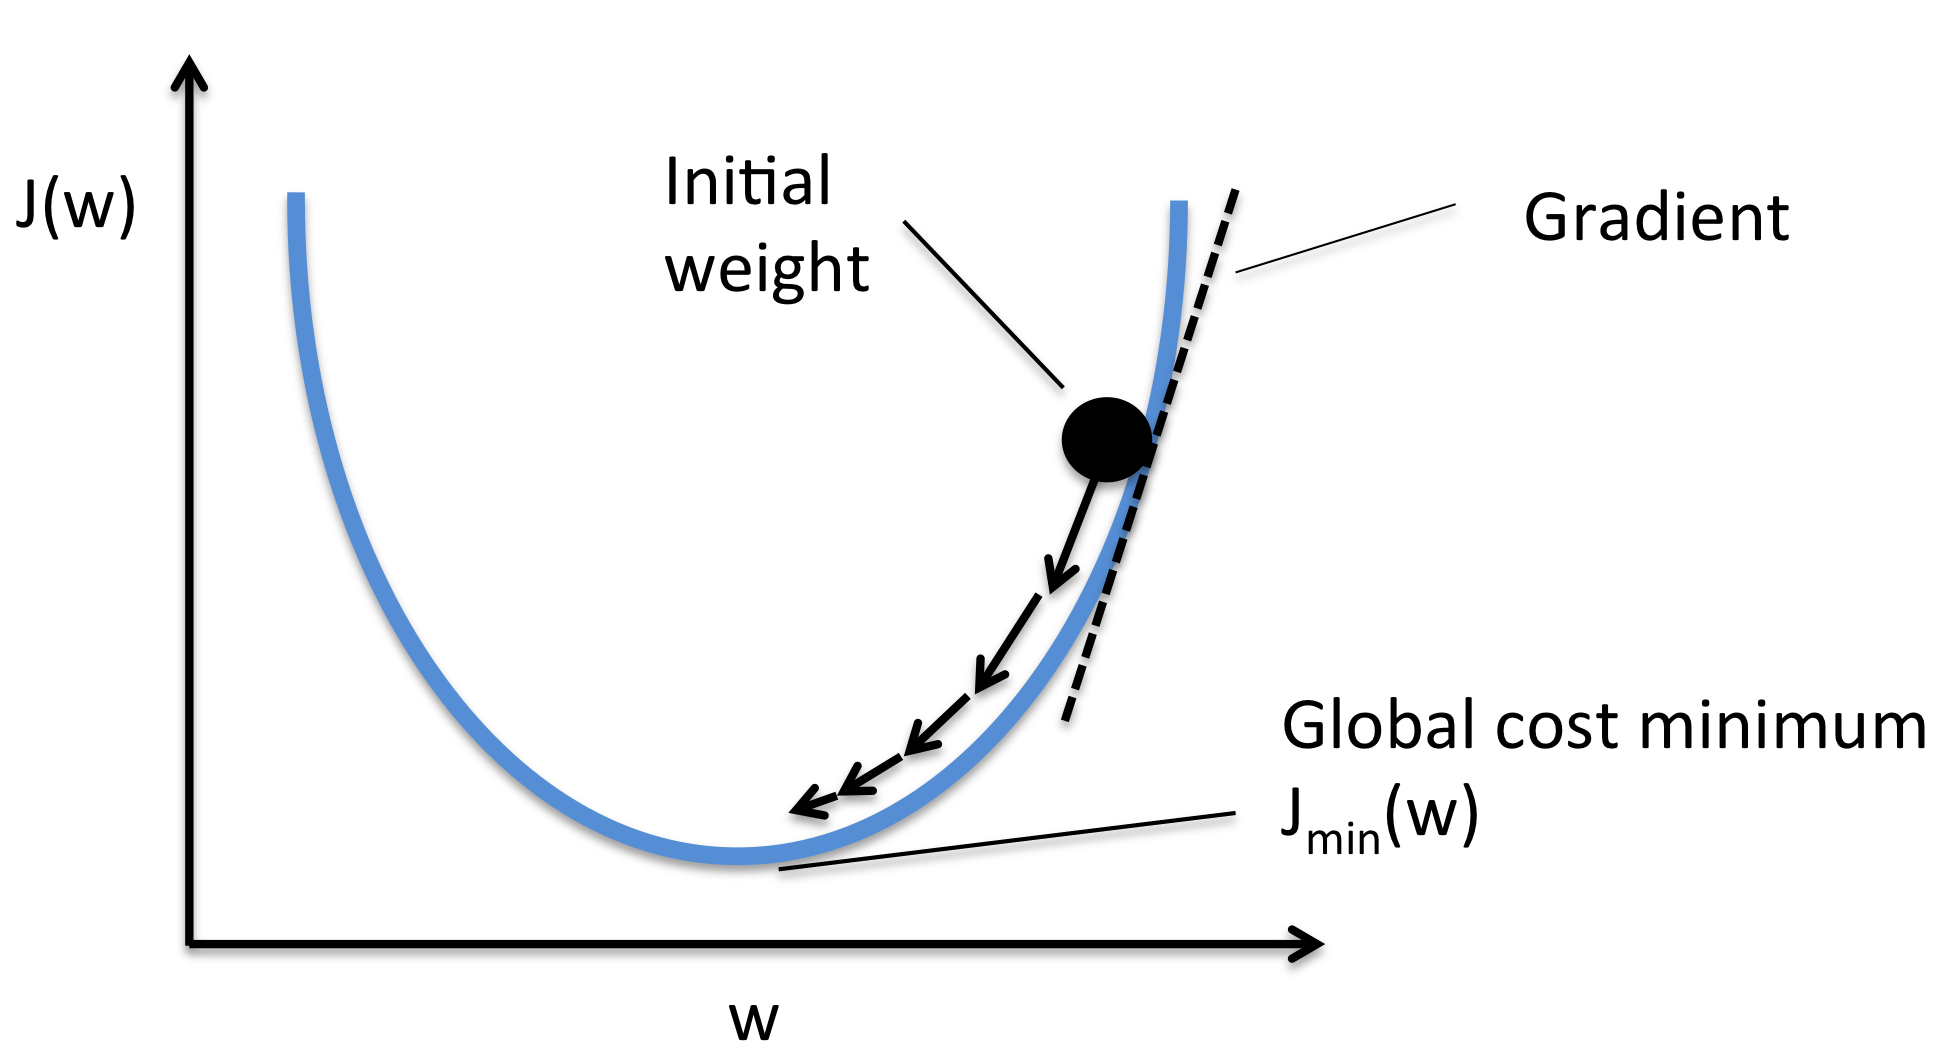
\includegraphics[width=0.7\columnwidth,keepaspectratio]{img/sgd.png}
	\caption{Visualisierung des Gradienten und der Loss-Funktion (J(w) = Loss; w = Parameteränderung)}
	\source{\url{http://rasbt.github.io/mlxtend/user_guide/general_concepts/gradient-optimization/} aufgerufen am: 05.08.2019}
	\label{fig:sgd}
\end{figure}
\subsubsection{Perceptron}
In der \cref{fig:perceptron-grafik} ist die Darstellung eines Perceptrons ersichtlich.
Ein Perceptron ist ein Knoten, welcher allen Input-Variablen \glqq x1-x3\grqq{} eine Gewichtung (Ein Mass für die Wichtigkeit) \glqq w1-w3\grqq{} zuweist.
Die gewichteten Inputs werden dann aufsummiert.
Wenn die Summe einen bestimmten Schwellwert überschreitet, schaltet der Ausgang \glqq y\grqq{} seinen Zustand um.\\
Ein einzelnes Perceptron kann als binärer Klassifizierer verwendet werden.
Im Deep-Learning Umfeld werden mehrere Perceptronen miteinander verbunden, um ein neuronales Netzwerk zu erstellen\footnote{\url{https://towardsdatascience.com/perceptron-the-artificial-neuron-4d8c70d5cc8d} abgerufen am: 05.08.2019}.
\begin{figure}[H]
	\centering	
	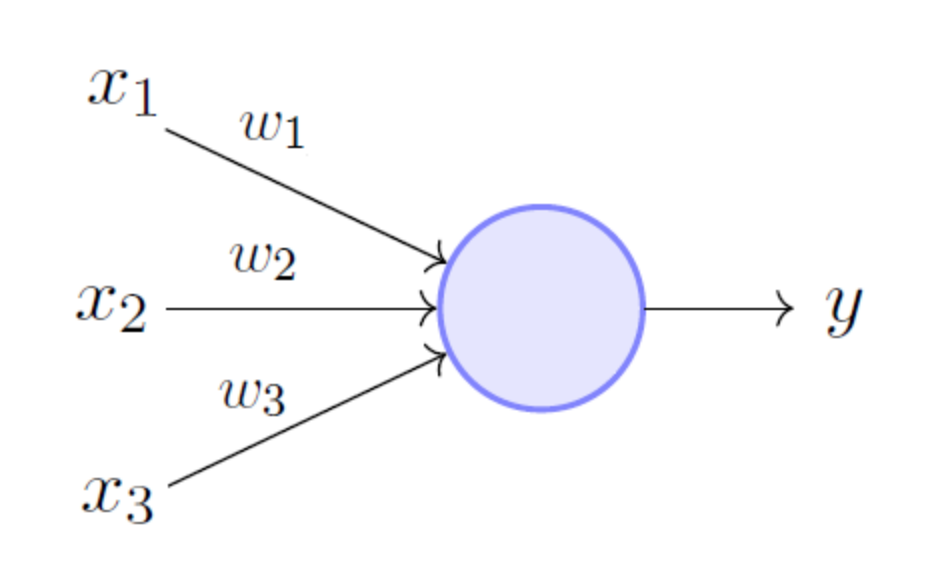
\includegraphics[width=0.6\columnwidth,keepaspectratio]{img/perceptron.png}
	\caption{Visualisierung eines Perceptrons}
	\source{\url{https://towardsdatascience.com/perceptron-the-artificial-neuron-4d8c70d5cc8d?} aufgerufen am: 05.08.2019}
	\label{fig:perceptron-grafik}
\end{figure}
\subsection{Naive Bayes}
Naive Bayes Algorithmen sind ein Set von Supervised Learning Algorithmen, welche auf dem Theorem von Bayes basieren.\\
Das Bayes Theorem zeigt die Berechnung von bedingten Wahrscheinlichkeiten auf:
$$ P(A \mid B) = \frac{P(B \mid A) \,* P(A)}{P(B)} $$
$$ P(A) = Wahrscheinlichkeit\ von\ Ereignis\ A$$
$$ P(B) = Wahrscheinlichkeit\ von\ Ereignis\ B$$
$$ P(A \mid B) = Wahrscheinlichkeit\ von\ Ereignis\ A\ nach\ eintreffen\ von\ Ereignis\ B$$
$$ P(B \mid A) = Wahrscheinlichkeit\ von\ Ereignis\ B\ nach\ eintreffen\ von\ Ereignis\ A$$
Das Bayes Theorem kann zur Hilfe genommen werden, um bedingte Ereignisse zu berechnen\footnote{\url{https://www.crashkurs-statistik.de/der-satz-von-bayes/} abgerufen am: 16.07.2019}.
Der naive Vorsatz deutet auf die Annahme des Theorems, dass eine vollständige Unabhängigkeit zwischen allen Features herrscht.
Diese Annahme ist in der realen Welt oft nicht korrekt, trotzdem können Naive Bayes Algorithmen gute Scores erreichen und werden oft als Referenz verwendet. \cite{rennie2003tackling}
\subsubsection{Multinomial Naive Bayes}
Der Multinomial Naive Bayes Algorithmus verwendet die Annahme, dass die unabhängigen Features einer Multinomialverteilung folgen.
Für jede Klasse werden Multinomial-Parameter bestimmt.
Diese Parameter sind Vektoren, welche die Wortwahrscheinlichkeiten, dass die Wörter in den entsprechenden Klassen vertreten sind, aufzeigen.
Die Wahrscheinlichkeit, dass ein Dokument zu einer Klasse gehört, wird mit dem Produkt aller Wortwahrscheinlichkeiten aus den Vektoren bestimmt, welche sich im Dokument befinden. \cite{rennie2003tackling}
\subsubsection{Gaussian Naive Bayes}
Der Gaussian Naive Bayes Algorithmus verwendet die Annahme, dass die unabhängigen Features einer Normalverteilung folgen\footnote{\url{https://scikit-learn.org/stable/modules/naive_bayes.html} abgerufen am: 16.07.2019} \cite{scikit-learn}.
\subsubsection{Bernoulli Naive Bayes}
Der Bernoulli Naive Bayes Algorithmus verwendet die Annahme, dass die unabhängigen Features einer Bernoulliverteilung folgen.
Die Features werden als binäre Vektoren dargestellt.
Somit wird nur das Vorhandensein und nicht die Häufigkeit der Features appliziert.
Ebenfalls werden alle Relationen zwischen den unterschiedlichen Features mit der strikten Einhaltung der binären Bernoulliverteilung entfernt. \cite{mccallum1998comparison}
\subsubsection{Complement Naive Bayes}
Der Complement Naive Bayes Algorithmus (CNB) ist eine Abwandlung des Multinomial Naive Bayes Algorithmus.
Er eignet sich für stark ungleiche Datensets und verwendet für das Setzen der internen Gewichte die Komplemente der einzelnen Klassen.
Das heisst, um die Gewichte für die Klasse A zu setzen, werden alle Klassen ausser A für die Berechnung der Gewichte verwendet. \cite{rennie2003tackling}
\subsection{DecisionTree}\label{sec:trees}
Der DecisionTree-Algorithmus baut schrittweise eine Baumstruktur von Entscheidungszweigen auf, um eine Klassifizierungsaufgabe zu meistern.
DecisionTrees versuchen eine komplexe Aufgabe in Teilprobleme zu zerlegen und diese mit einfachen Entscheidungen zu bewältigen.
DecisionTree-Strukturen können verbessert werden, indem die Tiefe der Äste oder die Anzahl der Äste angepasst wird.
Bei stetiger Erhöhung der Tiefe oder der Anzahl der Äste steigt auch die Zeitkomplexität der DecisionTrees. \cite{safavian1991survey}
\subsection{Ensemble-Learning}
Ensemble-Learning ist ein Zusammenschluss von mehreren unterschiedlichen Klassifizierern, welche mit einem Voting-Verfahren eine schlussendliche Klassifizierung durchführen.
Ensemble-Learning basiert auf der Annahme, dass mehrere Algorithmen im Plenum eine bessere Aussage liefern können als ein Algorithmus alleine. \cite{freund1999short}
\subsubsection{RandomForestClassifier}
RandomForest gehört ebenfalls zur Familie der Ensemble-Learner\footnote{\url{https://scikit-learn.org/stable/modules/generated/sklearn.ensemble.RandomForestClassifier.html} abgerufen am: 14.05.2019}.
RandomForest ist eine Zusammensetzung von mehreren unterschiedlichen DecisionTrees (siehe \cref{sec:trees}).\\
RandomForest verwendet nun eine Vielzahl von DecisionTrees, die alle unterschiedliche Tiefen oder Anzahl Äste besitzen.
Dadurch können Entscheidungsausreisser aufgefangen und durch den Mehrheitsentscheid gedämpft werden. \cite{liaw2002classification}
\subsubsection{AdaBoostClassifier}
Bei vielen Ensemble-Verfahren werden alle Klassifizierer parallel trainiert und geben ihr Votum gleichzeitig ab.
Adaboost verwendet jedoch die Methode des \glqq Boosting\grqq{}, welche Ähnlichkeit mit der Theorie der genetischen Algorithmen hat\footnote{\url{https://scikit-learn.org/stable/modules/ensemble.html} abgerufen am: 14.05.2019}.
Bei Adaboost wird ein Algorithmus trainiert, validiert und als Ursprung verwendet. Alle zusätzlichen Algorithmen, welche das finale Voting durchführen, werden vom Ursprungsalgorithmus abgeleitet.
Es werden jedoch bei den Abkömmlingen die internen Parameter schrittweise verbessert und versucht die Fehler des \glqq Vater-Algorithmus\grqq{} zu vermeiden.
AdaBoost kann verbessert werden, indem die Anzahl von Vererbungsschritten angepasst wird. \cite{freund1999short}
\subsection{Nearest Neighbor Modelle}
Der Nearest Neigbhor (NN) Algorithmus ist einer der simpelsten Entscheidungsprozesse für Klassifikationen.
Beim NN Algorithmus werden Datenpunkte entsprechend ihren nächsten Nachbarn klassifiziert. \cite{cover1967nearest}
Dieses Verhalten ist in der \cref{fig:knn} für unterschiedliche Schwellwerte der Anzahl Nachbarn ersichtlich.
\begin{figure}[H]
	\centering	
	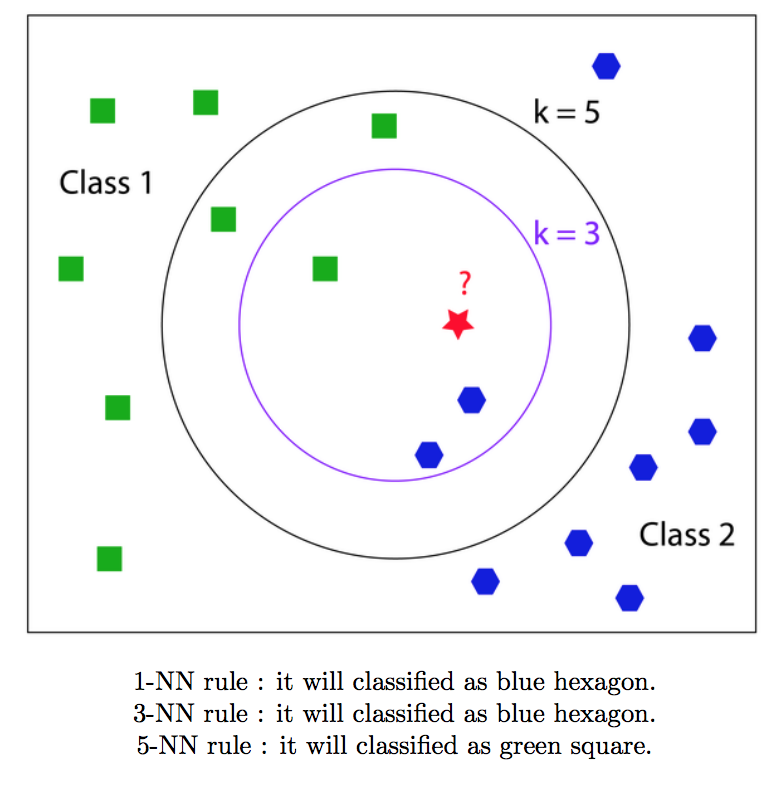
\includegraphics[width=0.7\columnwidth,keepaspectratio]{img/knn.png}
	\caption{Darstellung einer simplen K-Nearest Neighbor Prozedur}
	\source{\cite{cover1967nearest}}
	\label{fig:knn}
\end{figure}
\subsubsection{K-Nearest-Neighbor}
Der KNN Algorithmus funktioniert nach dem gleichen Prinzip wie der NN Algorithmus.
Ein Unterschied ist, dass eine spezifische Anzahl von Nachbarn mit der Kennzahl K definiert wird.
Alle K-nächsten Datenpunkten klassifizieren den gesuchten Datenpunkt mit einem Mehrheitsentscheid.
Dies ist in der \cref{fig:knn} für K=3 und K=5 ersichtlich.
K kann frei gewählt werden und dient hervorragend als Parameter für ein Hyperparametertuning (siehe \cref{sec:hyp}). \cite{cover1967nearest}
\subsubsection{Nearest Centroid}
Der Nearest Centroid Algorithmus basiert auf dem Prinzip des NN Algorithmus.
Zuerst werden die Schwerpunkte aller Klassen berechnet, indem alle zur Klasse zugewiesenen Datenpunkte miteinbezogen werden.
Danach wird der zu klassifizierende Datenpunkt der Klasse mit der kleinsten Differenz von Datenpunkt zu Schwerpunkt der Klasse zugewiesen.
Somit wird für den Nearest Centroid Algorithmus nicht der Mehrheitsentscheid der nächsten Nachbarn zur Klassifikation verwendet, sondern die Distanzen zu den Klassenschwerpunkten\footnote{\url{https://scikit-learn.org/stable/modules/neighbors.html} abgerufen am: 14.05.2019}. \cite{scikit-learn}
Dieses Verhalten ist in \cref{fig:centroid} ersichtlich.
Die schwarzen Datenpunkte markieren jeweils den Schwerpunkt der entsprechenden Klasse und die Abgrenzung der einzelnen Klassen ist mit gestrichenen, schwarzen Linien dargestellt.
\begin{figure}[H]
	\centering	
	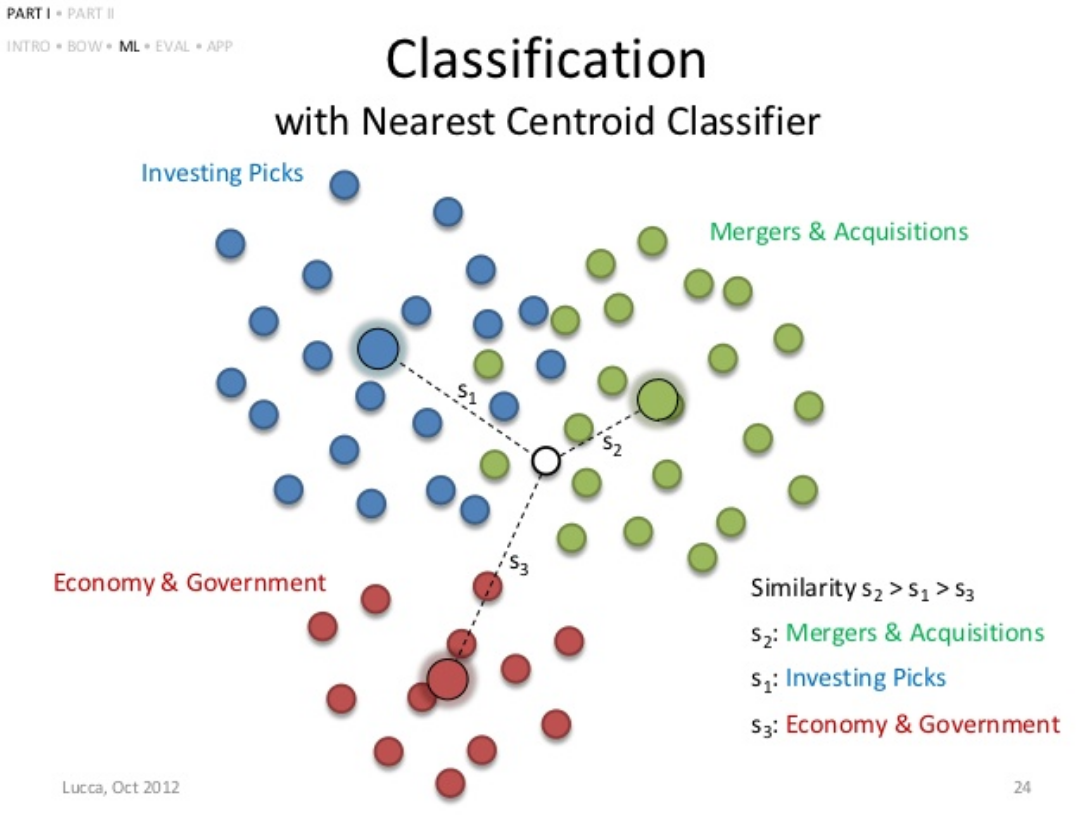
\includegraphics[width=0.7\columnwidth,keepaspectratio]{img/centroid.png}
	\caption{Darstellung einer simplen Nearest Centroid Prozedur}
	\source{\url{https://www.researchgate.net/figure/Abbildung-410-Illustration-des-Nearest-Centroid-Verfahrens-mit-den-Gruppen-soft_fig4_267488030} aufgerufen am: 14.05.2019}
	\label{fig:centroid}
\end{figure}
\subsection{Support Vector Machine Modelle}
SVM-Classifier (Support Vector Machine) erzielen gute Resultate bei der Klassifizierung von Textdateien.
Ein Vorteil von SVM ist, dass ihre Lernrate unabhängig von der Dimension der Features ist. \cite{joachims1998text}
Dies wird erreicht, da SVM nicht auf die ganzen Features angewiesen ist.
Zwischen den unterschiedlichen Klassen werden Hyperebenen gelegt, welche das Ziel haben, die Abstände zu den einzelnen Klassen zu maximieren.
In der \cref{fig:svm} ist eine solche Hyperebene ersichtlich.
Die Features, welche am nächsten zu den Hyperebenen liegen, werden Support Vektoren genannt.
Der Algorithmus kann nach der Trennung der Klassen nun die Position von neuen Features bestimmen und somit eine Schätzung einer geeigneten Klasse vornehmen. \cite{tong2001support}
\begin{figure}[H]
	\centering	
	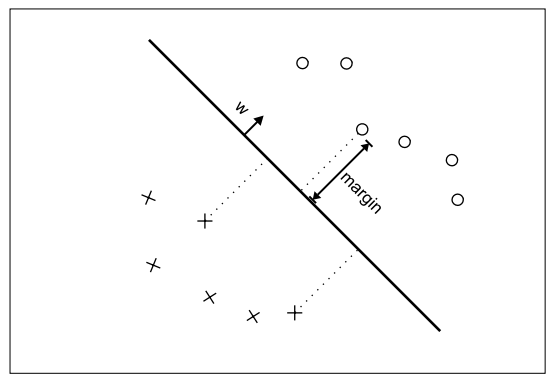
\includegraphics[width=0.7\columnwidth,keepaspectratio]{img/svm.png}
	\caption{Darstellung einer simplen Support Vector Machine}
	\source{\cite{tong2001support}}
	\label{fig:svm}
\end{figure}
\section{Hyperparametertuning}\label{sec:hyp}
Parameter, welche nicht selbstständig vom Machine-Learning Modell angepasst werden können, werden Hyperparameter genannt.
Diese Hyperparameter definieren das Verhalten von den Modellen.
Die geeignetsten Hyperparameter können mit einer ausführlichen Suche gefunden werden, was als Hyperparametertuning bezeichnet wird\footnote{\url{https://scikit-learn.org/stable/modules/grid_search.html} abgerufen am: 14.05.2019}. \cite{scikit-learn}
\newpage

\chapter{Methodik}
\section{Forschungsfrage}
Die Forschungsfrage, welcher mit dieser Arbeit beantwortet wird, lautet wie folgt:\\
\emph{Können Webpages von Restaurant-Websites mit hoher Erfolgschance klassifiziert werden, ob sie Menüinformationen beinhalten?}\\
Dabei handelt es sich um eine binäre Klassifikation, also eine Einteilung in zwei Kategorien, nämlich \glqq Menüseite\grqq oder \glqq Keine Menüseite\grqq.
Folgende Einschränkungen werden vorgegeben, um diese Frage beantworten zu können:
\begin{itemize}
	\item Die Webpages sind ausschliesslich von Restaurant-Websites
	\item Die Sprache der Webpages ist deutsch
\end{itemize}
\section{Ergebnisse der Klassifizierung}
In diesem Abschnitt wird zwischen zwei verschiedenen Ansätzen, namentlich dem regelbasierten und dem Klassifizieren mittels Machine-Learning unterschieden.
\subsection{Regelbasiertes Klassifizieren}
Die fünf verschiedenen Methoden des regelbasierten Klassifizierens haben folgende Ergebnisse erzielt:\\
\begin{tabular}{|l|l|l|l|}
	\hline
	Methode & F1-Score & Precision & Recall\\
	\hline
	Menü im Titel & 0.17 & 0.43 & 0.11 \\
	Preisdetektor & 0.46 & 0.45 & 0.47 \\
	Kombination aus Menü im Titel und Preisdetektor & 0.47 & 0.43 & 0.52\\
	Listing & 0.55 & 0.60 & 0.50\\
	Bag of Words & 0.72 & 0.81 & 0.64\\
	\hline
\end{tabular}\\
Hinweis: Wenn mehrere Parameterkombinationen denselben F1-Score erreicht haben, wurde diejenige mit der höheren Precision gewählt.
\subsection{Klassifizieren mittels Machine-Learning Algorithmen}
\section{Interpretation der Ergebnisse}
\subsection{Regelbasiertes Klassifizieren}
Die verschiedenen Methoden ergeben stark unterschiedliche Werte.
Die simpelste Methode, das Überprüfen des Schlagworts \glqq menu\grqq im Titel hat ein komplett unbrauchbares Ergebnis geliefert.
Dadurch kann gesagt werden, dass diese Art der Klassifizierung unbrauchbar ist.
Auch durch die Suche nach Preisen innerhalb eines Dokuments ist keine Klassifikation möglich, da es sowohl Menüseiten ohne Preisangaben gibt, aber auch viele weitere Webpages, die Preise beinhalten, aber keine Menüseiten sind.
Eine Kombination dieser beiden Methoden ergibt ebenfalls keine besseren Werte.
Das Verwenden einer Blacklist und Whitelist ergibt bessere Werte, jedoch auch nicht in einem Mass, welches für eine Klassifikation geeignet ist.
Diese würden sich verändern, wenn eine Änderung dieser Listen vorgenommen werden würden.
Ob dies zu einer Verbesserung oder Verschlechterung führt, lässt sich nicht pauschal sagen.
Die Klassifikation mit der Methode \glqq Bag of Words\grqq führt zu den besten Ergebnissen.
Dabei muss jedoch beachtet werden, dass ein Teil der Daten verwendet wird, um die dynamischen Listen zu erstellen.
Dadurch können die Werte nicht direkt mit denjenigen Methoden verglichen werden, welche die kompletten Daten klassifizieren. 
Insgesamt ist zu erkennen, dass eine qualitativ und quantitativ hochwertige Klassifikation von Texten unter diesen Umständen nicht möglich ist.
\subsection{Klassifizieren mittels Machine-Learning Algorithmen}
\section{Beantwortung der Forschungsfrage}
\newpage

\chapter{Teil 1: Gold Standard}
Als Rohdaten zur Erhebung dieses Gold Standards dient der Output des Webcrawlers.
Die Erarbeitung dieser Rohdaten kann im \cref{chap:engineering} nachgelesen werden.
\section{Seed}
Das Seed wurde als Datenquelle des Webcrawlers verwendet und bildet somit die Grundlage dieses Gold Standards.
Es wurde aus den folgenden zwei Quellen zusammengestellt:
\begin{itemize}
	\item OpenStreetMap - 3557 URLs
	\item Lunch-Check - 3803 URLs
\end{itemize}
Diese Quellen wurden verwendet, da sie diese Daten für diese Arbeit kostenlos zur Verfügung stellen.
Die URLs wurden zusammengeführt und Duplikate entfernt.
Daraus ist ein Seed entstanden, welches 5870 Einträge von Restaurant-URLs enthält.
Dabei wurden aus den nun aufgeführten Gründen mehrere Einträge entfernt:
\begin{itemize}
	\item Die Website enthält mehr als 300 Webpages
	\item Die Website ist offensichtlich keine Restaurant-Website
\end{itemize}
Websites mit mehr als 300 Webpages wurden entfernt, da diese keine typische Restaurant-Website repräsentieren und somit das Gesamtbild verzerren.
Es kann keine Gewähr gegeben werden, dass dieses Seed nur Restaurant-Websites beinhaltet, da nicht jeder Eintrag geprüft wurde.
\section{Entscheidungsraster}
Das Entscheidungsraster ist die Grundlage des manuellen Labeling der Rohdaten, daher wurde es als erstes erstellt.
Für dieses wurden die folgenden Entscheidungen getroffen:
\begin{itemize}
	\item Die Webpage muss auf Deutsch verfasst sein
	\item Der Anbieter muss entweder ein Restaurant, Take-Away oder Lieferdienst sein
	\item Der Text muss statisch im HTML vorhanden sein, da dynamisch gerenderte Informationen vom Webcrawler nicht gespeichert werden
	\item Es muss ein Menü, also eine Kombination aus mehreren Speisen oder eine einzelne Speise vorhanden sein
	\item Eine genauere Beschreibung oder der Preis muss vorhanden sein
	\item Getränkekarten werden explizit als negativ gelabelt
\end{itemize}
Bei der Klassifizierung wird zudem unterschieden, ob es sich um ein zeitlich begrenztes Angebot handelt, da diese Angebote zu einem späteren Zeitpunkt eventuell zusätzlich erkannt werden möchten.
\FloatBarrier
Der Gold Standard wurde anhand des Entscheidungsrasters erstellt, welches in der \cref{fig:classificationtree} dargestellt wird.
\begin{figure}	
	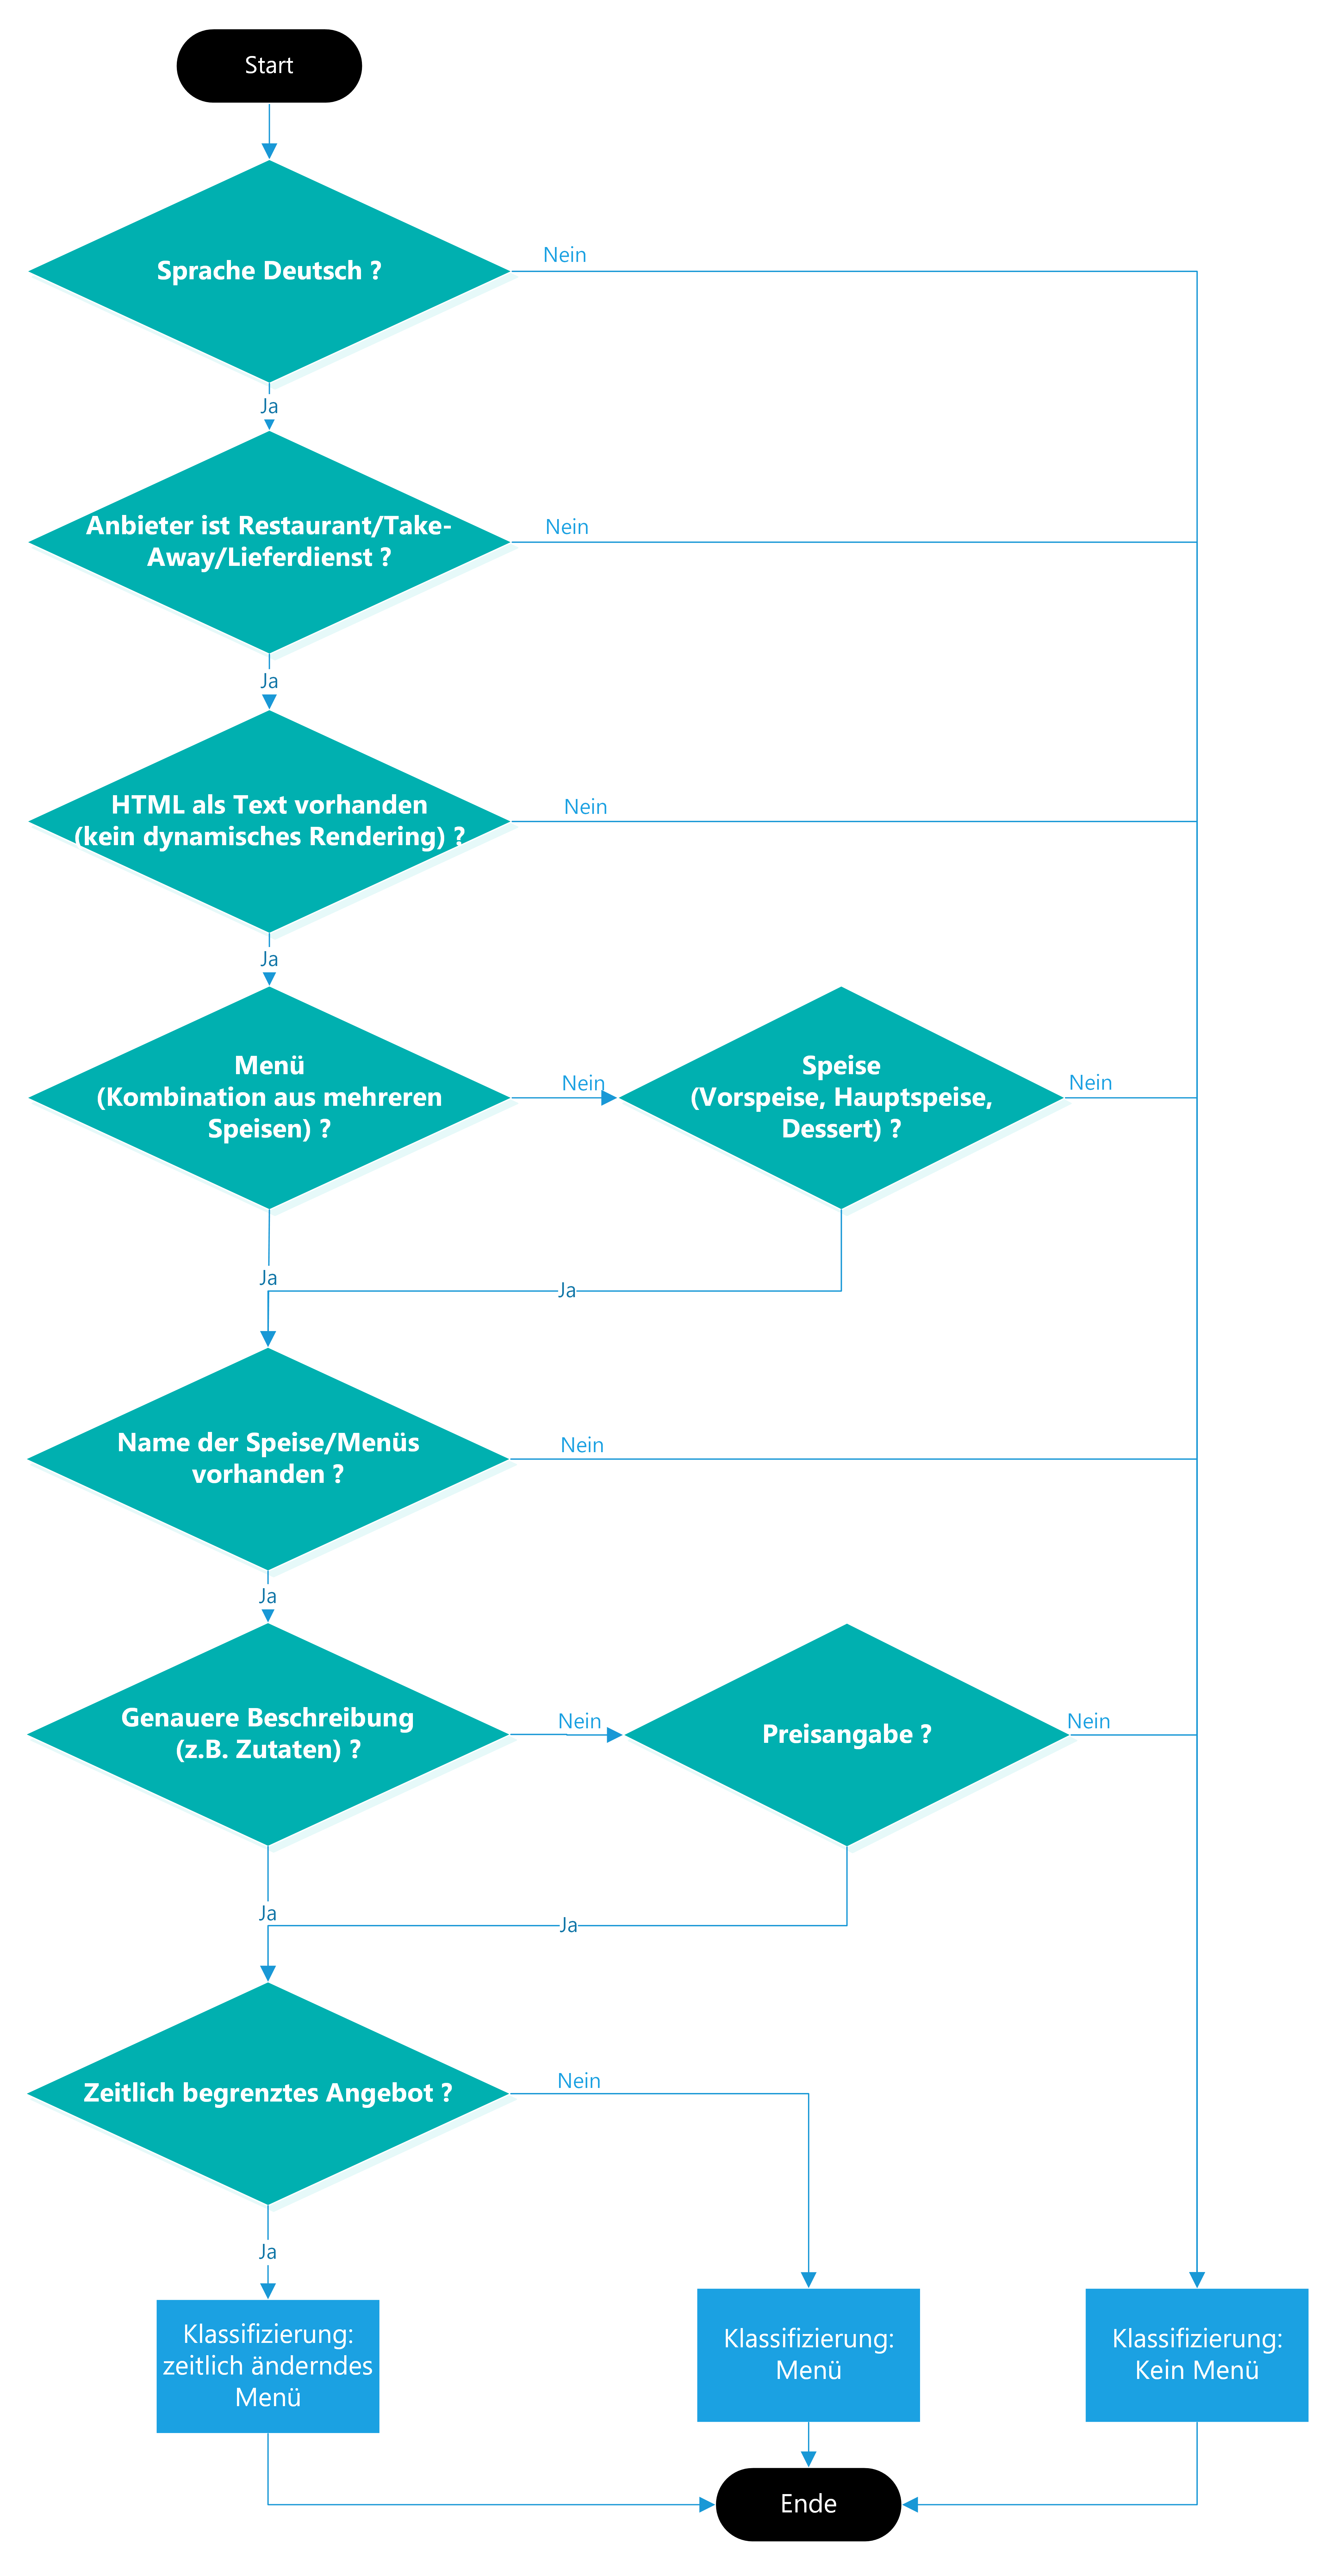
\includegraphics[width=0.65\columnwidth,keepaspectratio]{img/man-classification-tree.png}
	\caption{Entscheidungsraster}
	\label{fig:classificationtree}
\end{figure}
Obwohl bereits beim Webcrawler eine Spracherkennung eingesetzt wurde, damit nur als deutsch erkannte Webpages gespeichert werden, wurde bei der manuellen Klassifikation nochmals darauf geachtet, dass die Webpage in deutsch verfasst wurde.
Dabei ist anzumerken, dass gewisse Begriffe, vor allem für Speisebezeichnungen, auch fremdsprachig sein dürfen, da Speisebezeichnungen je nach Küche international ausgelegt sind.
Der Anbieter muss zwingend ein Restaurant, Take-Away oder Lieferdienst sein.
Der Inhalt muss statisch in der HTTP-Antwort verfügbar sein, da der Webcrawler nur diesen speichert und nicht mit dynamisch gerenderten Websites umgehen kann.
Der Name der Speise und eine genauere Beschreibung oder der Preis muss vorhanden sein.
Danach folgt die Unterscheidung zwischen zeitlich begrenzten und unbegrenzten Angeboten, welche zur Kategorisierung führt.
Getränkekarten wurden explizit negativ klassifiziert.

\section{Manuelles Labeling der Daten}
In einer ersten Durchführung des manuellen Labelings wurden ca. 1500 Dateien klassifiziert, welche das Schlüsselwort \glqq Menu\grqq{} in der URL enthalten.
Die mit dieser Heuristik gefilterten Daten entsprechen jedoch nicht einer repräsentativen Teilmenge der gesamten Rohdaten.
Darum wurde in einer zweiten Durchführung zufällig Proben aus den Rohdaten ausgewählt und manuell gelabelt.
Dadurch konnte sichergestellt werden, dass das Verhältnis von Menüseiten zu den restlichen Webpages gleich bleibt.
\subsection{Hilfsmittel: Labeling-Tool}
Um das manuelle Labeling effizienter zu gestalten, ist ein Tool\footnote{\url{https://github.com/s-santoro/testdata_tool} abgerufen am: 11.03.2019} erstellt worden, welches das Labeling vereinfacht.
Dieses Tool ruft eine Webpage der zufällig extrahierten Webpages aus den Rohdaten auf und zeigt sowohl den Text, als auch den HTML-Inhalt.
Der Anwender des Tools muss anhand dieser Informationen entscheiden, ob es sich um eine Webpage mit Menüinformationen handelt und ob diese zeitlich begrenzt sind.
Mittels Shortkeys findet die Klassifizierung statt.
Das Tool verschiebt die Datei in den entsprechenden Ordner und zeigt die Informationen der nächsten Webpage an.
\FloatBarrier
\section{Beschreibung des Gold Standards}
Der erarbeitete Gold Standard besteht insgesamt aus 6963 Dateien des Formats JSON, welche jeweils eine Webpage einer Restaurant-Website repräsentieren.
Diese Daten sind in einen Test- und einen Trainings- und Validierungsdatensatz unterteilt.
Der Gold Standard beinhaltet die folgenden drei Kategorien:
\begin{itemize}
	\item neg $\rightarrow$ Keine Menüseite
	\item pos\textunderscore daily\textunderscore menu $\rightarrow$ Zeitlich ändernde Menüseite
	\item pos\textunderscore menu $\rightarrow$ Menüseite
\end{itemize}
Die Datenstruktur des Gold Standards sieht wie folgt aus:\\

\begin{forest}
	for tree={
		font=\ttfamily,
		grow'=0,
		child anchor=west,
		parent anchor=south,
		anchor=west,
		calign=first,
		edge path={
			\noexpand\path [draw, \forestoption{edge}]
			(!u.south west) +(7.5pt,0) |- node[fill,inner sep=1.25pt] {} (.child anchor)\forestoption{edge label};
		},
		before typesetting nodes={
			if n=1
			{insert before={[,phantom]}}
			{}
		},
		fit=band,
		before computing xy={l=15pt},
	}
	[Gold Standard (6963 Dateien)
	[test (100 Dateien)
	[neg (50 Dateien)]
	[pos\textunderscore daily\textunderscore menu (10 Dateien)]
	[pos\textunderscore menu (40 Dateien)]
	]
	[train-validation (6863 Dateien)
	[neg (6257 Dateien)]
	[pos\textunderscore daily\textunderscore menu (87 Dateien)]
	[pos\textunderscore menu (519 Dateien)]
	]
	]
\end{forest}\\


Jeder Eintrag dieses Gold Standards beinhaltet die folgenden Informationen:
\begin{itemize}
	\item \glqq date\grqq{} - Zeitpunkt, zu welchem die Webpage aufgerufen wurde
	\item \glqq text\grqq{} - Vom Webcrawler extrahierter Text, welcher die Webpage beinhaltet
	\item \glqq encoding\grqq{} - Das von der Webpage verwendete Encoding
	\item \glqq title\grqq{} - Inhalt des gleichnamigen HTML-Metatags
	\item \glqq url\grqq{} - URL der Webpage
	\item \glqq content\grqq{} - Der statische HTML-Inhalt der Webpage	
\end{itemize}



\newpage

\chapter{Teil 2: Klassifikation}
\section{Einleitung}\label{sec:classification}
Um eine Klassifizierung durchführen zu können, sind mehrere Komponenten notwendig, welche miteinander arbeiten. 
Dieser Ablauf wird in der \cref{fig:ablauf_klassifizierung} gezeigt.
\begin{figure}[H]
	\centering	
	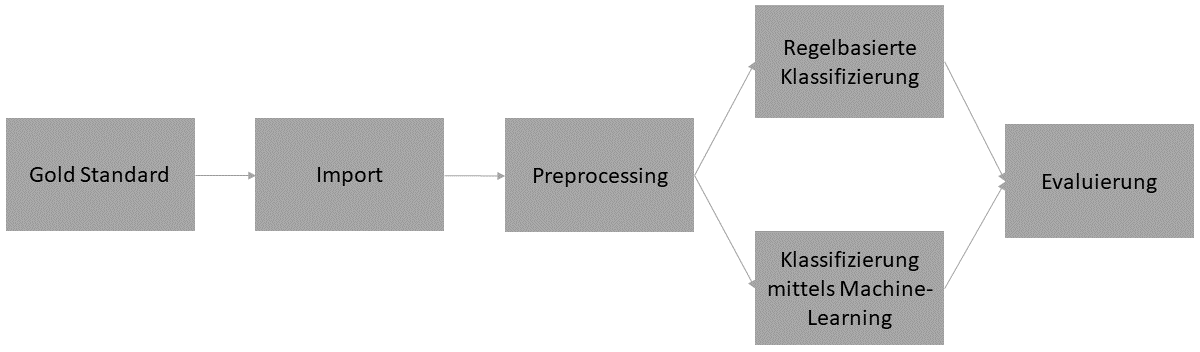
\includegraphics[width=1\columnwidth,keepaspectratio]{img/Ablauf_Klassifizierung.png}
	\caption{Pipeline}
	\source{Eigene Darstellung}
	\label{fig:ablauf_klassifizierung}
\end{figure}
Als Grundlage dienen die Daten des Gold Standards.
Diese werden mittels einer Import-Komponente geladen.
Bevor die Daten mit den entsprechenden Methoden klassifiziert werden, werden sie bei Bedarf noch vorverarbeitet.
Dann findet die eigentliche Klassifizierung statt.
Um eine möglichst präzise und erfolgreiche Variante des Klassifizierens zu finden, werden in diesem Teil der Arbeit mehrere Experimente durchgeführt.
Zum Schluss folgt eine Komponente, welche für das Auswerten der Klassifizierung und Ausgeben der Ergebnisse verantwortlich ist.
Bei dieser Klassifikation wird nicht zwischen den Kategorien \glqq Menüseite\grqq{} und \glqq Zeitlich ändernde Menüseite\grqq{} des Gold Standards unterschieden.
Diese Kategorien wurden zu einer Kategorie \glqq Menüseite\grqq{} zusammengeführt.
\section{Verwendete Technologien}
Folgend werden Technologien aufgelistet, welche einen hohen Stellenwert bei der Durchführung der Experimente eingenommen haben.
\subsection{Luigi}
Luigi ist ein Pipelining-Tool, welches vom Musikstreamingdienst Spotify entwickelt und später als Open-Source Projekt veröffentlicht worden ist\footnote{\url{https://github.com/spotify/luigi} abgerufen am 25.03.2019}.
Pipelining dient dazu, mehrere Tasks miteinander zu verknüpfen, das Ausführen zu Automatisieren und somit eine grössere Aufgabe zu verrichten.
Pipelining wird meist im Kontext von Big Data oder Machine-Learning angewendet, wo sich viele einzelne Tasks mit grossen Datenmengen beschäftigen.
Luigi wird selbst von Spotify selbst in der produktiven Umgebung verwendet und bietet unter anderem folgende Features:
\begin{itemize}
	\item Einzelne Tasks idempotent ausführen
	\item Teilschritte oder gesamte Pipeline kann über Konsolenausgabe oder Webinterface überwacht werden
	\item Fehlerfälle können protokolliert und dementsprechend reagiert werden
	\item Abhängigkeiten von Tasks werden selbstständig von Luigi gelöst
	\item Luigi ist komplett in Python aufgebaut und kann auch mit Python konfiguriert werden
\end{itemize}
Die einzelnen Tasks werden mit Python-Klassen realisiert.
Luigi ist so aufgebaut, dass jeder Task ein Input-File liest, von dem die Ausgabe des vorherigen Tasks eingelesen wird und ein Output-File schreibt, welches als Input-File des anschliessenden Tasks benutzt wird.
Dadurch kann Luigi die Zustände der einzelnen Tasks überwachen und im Falle eines Fehlers die Pipeline dort wieder starten, wo sie abgebrochen wurde.
Damit Luigi die Abhängigkeiten und das Überwachen bewerkstelligen kann, benötigt jede Klasse in der Pipeline folgende drei Funktionen:
\begin{itemize}
	\item Funktion requires() - Angabe auf welche Tasks Abhängigkeiten bestehen
	\item Funktion run() - Bereich, wo die eigentliche Logik des Tasks ist
	\item Funktion output() - Angabe, wohin die Ausgabe geschrieben wird
\end{itemize}
In dieser Arbeit wurde Luigi verwendet, um die einzelnen Tasks der Klassifizierung zu verknüpfen.

Es wurden zwei verschiedene Arten von Pipelines erstellt.
Die Entwicklungspipeline diente zur Entwicklung der Regeln/Machine-Learning-Modelle für die Klassifizierung.
Die Pipeline beinhaltet das Lesen der gecrawlten Daten, das Preprocessing, das Klassifizieren und das Evaluieren der Klassifizierung.
Sie beinhaltet folgende Komponenten:
\begin{itemize}
	\item Importer - Importiert die gecrawlten Websites und speichert sie in einer CSV-Datei
	\item Preprocessor - Wendet Preprocessing-Schritte an den Daten an
	\item RuleBasedClassifier - Regelbasierte Klassifizierung der Daten 
	\item MLClassifier - Klassifizierung der Daten mittels Machine-Learning
	\item Evaluator - Auswertung der Klassifizierung von Daten (nur im Entwicklunsmodus)
\end{itemize}
Die Produktionspipeline diente zur schlussendlichen Klassifizierung der Rohdaten anhand eines in der Entwicklungspipeline evaluierten Algorithmus.
\subsection{Scikit Learn}
Scikit Learn ist eine freie Programmierbibliothek für Python, mit welcher effizient Projekte für Data-Mining, Datenvisualisierung und Machine-Learning erarbeiten kann.
Scikit Learn ist unter BSD lizenziert und für die kommerzielle Nutzung frei verfügbar.
Sie ist eine der bekanntesten Standardbibliotheken für Machine-Learning, wird unter anderem von grossen Namen wie Google finanziell unterstützt und besitzt eine rege Contribution-Community auf Github\footnote{\url{https://github.com/scikit-learn/scikit-learn} abgerufen am: 07.05.2019}.\\
Scikit Learns Stärken liegen in den Machine-Learning Bereichen \glqq Supervised Learning\grqq{} und \glqq Unsupervised Learning\grqq{}.
Die API von Scikit Learn bietet eine Vielzahl von Algorithmen für Klassifizierung, Regression, Clustering, Dimensionsreduktion, Modelselektion sowie Preprocessing an und deckt somit die ganze Machine-Learning Pipeline ab\footnote{\url{https://scikit-learn.org/stable/} abgerufen am: 07.05.2019}.
Scikit Learn bietet für fast jeden Algorithmus oder Technik in der API eine Beispielimplementation an, welche für Fast-Prototyping  als Fundament übernommen werden kann.\\
Scikit-Learn wurde sowohl in der regelbasierten Klassifikation, als auch in der Klasssifikation mittels Machine-Learning verwendet.
\section{Preprocessing}
Das Preprocessing wurde entwickelt, um den Inhalt des Dokuments in eine standardisierte Form zu bringen.
Die folgenden Methoden können sowohl auf den Text eines Dokuments sowie auch auf den Titel angewendet werden.
Sie können mittels Konfiguration sowohl für den Text als auch Titel eines Dokuments ein- oder ausgeschaltet werden.
Der Link zum entsprechenden Code ist im \cref{app:classification} zu finden.
\subsection{Basis Preprocessing}
Um Text besser klassifizieren zu können, muss dieser zuerst bereinigt und standardisiert werden\footnote{\url{https://machinelearningmastery.com/clean-text-machine-learning-python/} abgerufen am: 11.07.2019}.
Die nachfolgenden Methoden des Basis Preprocessing werden in jedem Fall der Klassifikation durchgeführt.
Sie verändern jeweils nur einzelne Zeichen des Textes.
\subsubsection{Gross-/Kleinschreibung}
Alle Buchstaben, welche grossgeschrieben sind, werden durch die entsprechenden Kleinbuchstaben ersetzt.
\subsubsection{Umlaute ersetzen}
Umlaute werden durch ihre verwandten Selbstlaute ersetzt, genauer:
\begin{itemize}
	\item ä $\rightarrow$ a
	\item ö $\rightarrow$ o
	\item ü $\rightarrow$ u
\end{itemize} 
\subsubsection{Sonderzeichen entfernen}
Alle Sonderzeichen, die nicht in der folgenden Auflistung vorkommen, werden durch einen Leerschlag ersetzt:
\begin{itemize}
	\item éàèÉÀÈäöüÄÖÜa-zA-Z
\end{itemize} 
\subsubsection{Einzelne Zeichen entfernen}
Jedes einzelne Zeichen, also solche, die sowohl vorne als auch hinten an einen Leerschlag angrenzen, werden entfernt.
\subsubsection{Multiple Leerschläge entfernen}
Da durch die vorhergehenden Schritte oft multiple Leerschläge anfallen, werden diese auf einen Leerschlag reduziert.
\subsection{Fortgeschrittenes Preprocessing}\label{sec:advancedpre}
Die nachfolgenden Methoden stellen das fortgeschrittene Preprocessing dar.
Im Gegensatz zum Basis Preprocessing ersetzen, löschen oder verändern sie ganze Wörter im Text.
\subsubsection{Preisdetektor}
Da Menüs häufig in Verbindung mit Preisen vorkommen und in weiteren Preprocessing-Schritten Zahlen und Sonderzeichen entfernt werden, ist es von Vorteil, diese Informationen nicht zu verlieren.
Daher erkennt diese Methode verschiedene Varianten von Preisen mittels regulären Ausdrücken (Regex, Regular Expression) und ersetzt diese mit einem Schlüsselwort.
% Varianten genauer ausführen
Die folgenden Varianten von Preisen wird erkannt:
\begin{itemize}
	\item Preisangabe + chf/fr/sfr
	\item Preisangabe
	\item chf/fr/sfr + Preisangabe
\end{itemize} 
Zudem wird unterschieden, wie viele Stellen der Preis hat.
Die nun aufgeführte Liste zeigt die verschiedenen Schlüsselwörter:
\begin{itemize}
	\item Einstellig $\rightarrow$ onedigitprice
	\item Zweistellig $\rightarrow$ twodigitprice
	\item Dreistellig $\rightarrow$ threedigitprice
\end{itemize} 
Um Zeitangaben nicht als Preise zu erkennen, werden bei Preisangaben ohne Währungsangabe nur Beträge mit Rappenbeträgen, welche 60 oder höher sind, erkannt.
\subsubsection{Stammformreduktion}
Dieses Verfahren führt verschiedene morphologische Varianten eines Wortes auf ihren gemeinsamen Stamm zurück.
Dafür wird der Stemmer \glqq Cistem\footnote{\url{https://github.com/LeonieWeissweiler/CISTEM} abgerufen am: 18.03.2019}\grqq{} verwendet, da für die deutsche Sprache nur wenig Alternativen vorhanden sind.
Ein Beispiel: Die Wörter \glqq Preise\grqq{} und \glqq Preisen\grqq{} werden beide auf \glqq Preis\grqq{} reduziert.
\subsubsection{Getränkedetektor}
% Referenz Cistem
Eine Liste mit Einträgen diverser Getränke bildet die Grundlage dieser Methode.
Wenn im Text ein Getränk dieser Liste vorhanden ist, wird es durch das Schlüsselwort \glqq beverageentity\grqq{} ersetzt.
Damit soll erreicht werden, dass ein einheitliches Merkmal geschaffen wird.
\subsubsection{Stoppwörter entfernen}
Bei Stoppwörter handelt es sich um Wörter, welche keine Relevanz für den Inhalt eines Texts haben, aber oft vorkommen, wie z.B. \glqq in\grqq{}, \glqq auf\grqq{} und \glqq oder\grqq{}.
Eine Stoppwortliste führt 1720 solcher Wörter in Deutsch auf. Sie ist aus mehreren Quellen zusammengesetzt worden.
Wenn eines dieser Wörter im Text vorkommt, wird es entfernt.
\section{Regelbasierte Experimente}
Die folgenden Experimente beschreiben die Methoden und Resultate der regelbasierten Experimente.
Anschliessend folgt die Interpretation und Diskussion.
Der Link zum entsprechenden Code ist im Anhang (\cref{app:classification}) zu finden.
\subsection{Regelsatz: Menü im Titel}
\subsubsection{Methode}
Dieser simple Algorithmus überprüft, ob der Begriff \glqq menu\grqq{} in einem Wort des Metatags \glqq Title\grqq{} vorkommt.
Falls ja, wird das Dokument als Menüseite klassiert.
\subsubsection{Resultate}
Für dieses Regelset sind keine Parameter verfügbar, daher ist nur eine Konfiguration durchgeführt worden.
Diese hat anhand der Trainingsdaten folgende Metriken ergeben:\\
\begin{table}[H]
	\centering
	\begin{tabular}{|l|l|l|}
		\hline
		F1-Score & Precision & Recall\\
		\hline
		0.17 & 0.43 & 0.11  \\
		\hline
	\end{tabular}
	\caption{Score des Regelsets: Menü im Titel anhand der Trainingsdaten}
\end{table}
Das folgende Ergebnis ist anhand der Daten des Testsets entstanden:
\begin{table}[H]
	
	\centering
	\begin{tabular}{|l|l|l|l|}
		\hline
		Methode & F1-Score & Precision & Recall\\
		\hline
		Menü im Titel & 0.28 & 1.00 & 0.16 \\
		\hline
	\end{tabular}
	\caption{Score des Regelsatzes: Menü im Titel anhand der Testdaten}
\end{table}
Die Klassifizierung in absoluten Zahlen wird mittels Konfusionsmatrix verdeutlicht.
\begin{table}[H]
	\centering
	\begin{tabular}{@{}cc|cc@{}}
		\multicolumn{1}{c}{} &\multicolumn{1}{c}{} &\multicolumn{2}{c}{Predicted} \\ 
		\multicolumn{1}{c}{} & 
		\multicolumn{1}{c|}{} & 
		\multicolumn{1}{c}{Positiv} & 
		\multicolumn{1}{c}{Negativ} \\ 
		\cline{2-4}
		\multirow[c]{2}{*}{\rotatebox[origin=tr]{90}{Actual}}
		& Positiv  & 8   & 42   \\[1.5ex]
		& Negativ  & 0   & 50 \\ 
		\cline{2-4}
	\end{tabular}
	\caption{Konfusionsmatrix des Regelsets: Menü im Titel anhand der Testdaten}
\end{table}
\subsection{Regelsatz: Preisdetektor}
\subsubsection{Methode}
Dieser Algorithmus funktioniert dank der Preprocessing-Methode, welche den Preis erkennt und mit einem Schlüsselwort ersetzt.
Sofern dieses Schlüsselwort für zweistellige Preise im Text vorhanden ist, wird das Dokument als Menüseite klassifiziert. 
Dies unter der Annahme, dass Menüpreise oft zweistellig, im Gegensatz zu Getränkepreisen welche häufig einstellig und Hotelpreisen, die meist dreistellig sind.
Die Anzahl vorhandener Preise kann über die Konfiguration angegeben werden.
\subsubsection{Resultate}
Durch die Konfiguration kann ein Schwellwert für die Anzahl erkannter Preise angegeben werden, die vorhanden sein müssen, um eine Webpage als positiv zu klassifizieren.\\
\begin{table}[H]
	\centering
	\begin{tabular}{|l|l|l|l|}
		\hline
		Schwellwert & F1-Score & Precision & Recall\\
		\hline
		1 & 0.45 & 0.36 & 0.60  \\
		2 & 0.46 & 0.45 & 0.47 \\
		3 & 0.41 & 0.49 & 0.36 \\
		\hline
	\end{tabular}
	\caption{Scores des Regelsets: Preisdetektor anhand der Trainingsdaten}
\end{table}
Das beste Ergebnis hat ein Schwellwert von zwei erzielt, danach ist der F1-Score wieder schlechter geworden.
Daraus wurde geschlussfolgert, dass für dieses Regelset das Maximum bereits erreicht wurde.
\\
Das folgende Ergebnis ist anhand der Daten des Testsets entstanden:
\begin{table}[H]
	\centering
	\begin{tabular}{|l|l|l|l|}
		\hline
		Methode & F1-Score & Precision & Recall\\
		\hline
		Preisdetektor & 0.65 & 0.93 & 0.50 \\
		\hline
	\end{tabular}
	\caption{Score des Regelsatzes: Preisdetektor anhand der Testdaten} 
\end{table}
Die Klassifizierung in absoluten Zahlen wird mittels Konfusionsmatrix verdeutlicht.
\begin{table}[H]

	\centering
	\begin{tabular}{@{}cc|cc@{}}
		\multicolumn{1}{c}{} &\multicolumn{1}{c}{} &\multicolumn{2}{c}{Predicted} \\ 
		\multicolumn{1}{c}{} & 
		\multicolumn{1}{c|}{} & 
		\multicolumn{1}{c}{Positiv} & 
		\multicolumn{1}{c}{Negativ} \\ 
		\cline{2-4}
		\multirow[c]{2}{*}{\rotatebox[origin=tr]{90}{Actual}}
		& Positiv  & 25   & 25   \\[1.5ex]
		& Negativ  & 2    & 48 \\ 
		\cline{2-4}
	\end{tabular}
	\caption{Konfusionsmatrix des Regelsets: Preisdetektor anhand der Testdaten}
\end{table}
\subsection{Regelsatz: Kombination aus Menü im Titel und Preisdetektor}
\subsubsection{Methode}
Diese Kombination führt eine sequenzielle Klassifikation aus.
Im ersten Schritt wird der Mechanismus des Algorithmus \glqq Menü im Titel\grqq{} verwendet.
Falls durch diesen keine positive Klassifikation zustande kommt, wird durch den Preisdetektor nochmals neu klassifiziert.
\subsubsection{Resultate}
Bei dieser Konfiguration kann der Schwellwert ebenfalls für die Anzahl erkannter Preise angegeben werden.\\
\begin{table}[H]
	\centering
	\begin{tabular}{|l|l|l|l|}
		\hline
		Schwellwert & F1-Score & Precision & Recall\\
		\hline
		1 & 0.45 & 0.35 & 0.65 \\
		2 & 0.47 & 0.43 & 0.52 \\
		3 & 0.43 & 0.45 & 0.41 \\
		\hline
	\end{tabular}
	\caption{Scores des Regelsets: Kombination aus Menü im Titel und Preisdetektor anhand der Trainingsdaten}
\end{table}
Auch bei diesem Regelset hat die Konfiguration mit einem Schwellwert von zwei das beste Ergebnis erzielt.
\\
Das folgende Ergebnis ist anhand der Daten des Testsets entstanden:
\begin{table}[H]
	\centering
	\begin{tabular}{|l|l|l|l|}
		\hline
		Methode & F1-Score & Precision & Recall\\
		\hline
		Kombination aus Menü im Titel und Preisdetektor & 0.70 & 0.93 & 0.56\\
		\hline
	\end{tabular}
	\caption{Score des Regelsatzes: Kombination aus Menü im Titel und Preisdetektor anhand der Testdaten}
\end{table}
Die Klassifizierung in absoluten Zahlen wird mittels Konfusionsmatrix verdeutlicht.
\begin{table}[H]
	\centering
	\begin{tabular}{@{}cc|cc@{}}
		\multicolumn{1}{c}{} &\multicolumn{1}{c}{} &\multicolumn{2}{c}{Predicted} \\ 
		\multicolumn{1}{c}{} & 
		\multicolumn{1}{c|}{} & 
		\multicolumn{1}{c}{Positiv} & 
		\multicolumn{1}{c}{Negativ} \\ 
		\cline{2-4}
		\multirow[c]{2}{*}{\rotatebox[origin=tr]{90}{Actual}}
		& Positiv  & 28   & 22   \\[1.5ex]
		& Negativ  & 2   & 48 \\ 
		\cline{2-4}
	\end{tabular}
	\caption{Konfusionsmatrix des Regelsets: Kombination aus Menü im Titel und Preisdetektor anhand der Testdaten}
\end{table}
\subsection{Regelsatz: Listing}
\subsubsection{Methode}
Dieser Algorithmus basiert sowohl auf dem Blacklisting- als auch auf dem Whitelisting-Ansatz.
Dazu wird eine Blacklist und eine Whitelist verwendet, die von Hand erstellt wurden und Einträge enthalten, welche für die jeweiligen Kategorien typisch sind.
Falls ein Wort aus der Black- oder Whitelist im Text einer Webpage vorkommt, wird ein entsprechender Zähler hochgezählt.
Zum Schluss findet eine sequenzielle Klassifizierung statt, das heisst: 
Wenn der Zähler der Blacklist einen konfigurierbaren Schwellwert überschreitet, wird die Webpage als negativ klassifiziert. 
Wenn der Zähler der Whitelist einen konfigurierbaren Schwellwert überschreitet, wird die Webpage als Menüseite klassifiziert.
Falls keiner der beiden Zähler den Schwellwert überschreitet, wird die Webpage ebenfalls als negativ klassifiziert. 
\subsubsection{Resultate}
In einem ersten Versuch wurden identische Schwellwerte gewählt und jeweils erhöht:\\
\begin{table}[H]
	\centering
	\begin{tabular}{|l|l|l|l|l|}
		\hline
		Schwellwert Whitelist & Schwellwert Blacklist & F1-Score & Precision & Recall\\
		\hline
		1 & 1 & 0.17 & 0.32 & 0.11 \\
		5 & 5 & 0.39 & 0.62 & 0.29 \\
		10 & 10 & 0.42 & 0.77 & 0.29 \\
		20 & 20 & 0.33 & 0.85 & 0.21 \\
		30 & 30 & 0.27 & 0.91 & 0.16 \\
		\hline
	\end{tabular}
	\caption{Scores der ersten Iteration des Regelsets: Listing anhand der Trainingsdaten}
\end{table}
Dieser Versuch hat gezeigt, dass ein maximaler F1-Score bei gleichen Werten zwischen 5 und 20 zu erreichen ist.\\
Da gleich gewählte Werte keine zufriedenstellende Ergebnisse erzielten, wurden im zweiten Versuch unterschiedliche Verhältnisse getestet:\\
\begin{table}[H]
	\centering
	\begin{tabular}{|l|l|l|l|l|}
		\hline
		Schwellwert Whitelist & Schwellwert Blacklist & F1-Score & Precision & Recall\\
		\hline
		5 & 1 & 0.12 & 0.82 & 0.07 \\
		1 & 5 & 0.31 & 0.24 & 0.45 \\
		\hline
	\end{tabular}
	\caption{Scores der zweiten Iteration des Regelsets: Listing anhand der Trainingsdaten}
\end{table}
Aus diesem Versuch entstand die Erkenntnis, dass ein höherer Schwellwert der Blacklist als der Whitelist erforderlich ist, um einen möglichst hohen Score zu erreichen.
Diese Erkenntnis wurde in einem weiteren Versuch in mehreren Iterationen getestet:\\
\begin{table}[H]
	\centering
	\begin{tabular}{|l|l|l|l|l|}
		\hline
		Schwellwert Whitelist & Schwellwert Blacklist & F1-Score & Precision & Recall\\
		\hline
		2 & 10 & 0.42 & 0.33 & 0.61 \\
		3 & 15 & 0.52 & 0.42 & 0.70 \\
		3 & 20 & 0.51 & 0.39 & 0.75 \\
		4 & 15 & 0.53 & 0.47 & 0.61 \\
		5 & 15 & 0.55 & 0.54 & 0.56 \\
		5 & 20 & 0.54 & 0.50 & 0.60 \\
		5 & 21 & 0.54 & 0.49 & 0.60 \\
		6 & 20 & 0.55 & 0.56 & 0.55 \\
		7 & 20 & 0.55 & 0.60 & 0.50 \\
		8 & 20 & 0.53 & 0.64 & 0.46 \\
		\hline
	\end{tabular}
	\caption{Scores der dritten Iteration des Regelsets: Listing anhand der Trainingsdaten}
\end{table}
Die Schwellwerte wurden stetig erhöht.
Dabei wurden verschiedene Schwellwerte in unterschiedlichen Verhältnissen getestet.
Sobald einer dieser Schwellwerte zu einem schlechteren Ergebnis geführt hat, wurde er wieder reduziert oder ein neues Verhältnis getestet.
Beim Verhältnis 6/20 bzw. 7/20 wurde das Maximum des F1-Scores erreicht.
Da diese Werte nicht im Bereich einer zufriedenstellenden Klassifikation sind, wurde auf die Ermittlung aller möglichen Kombinationen verzichtet.
\\
Das folgende Ergebnis ist anhand der Daten des Testsets entstanden:
\begin{table}[H]
	\centering
	\begin{tabular}{|l|l|l|l|}
		\hline
		Methode & F1-Score & Precision & Recall\\
		\hline
		Listing & 0.68 & 0.96 & 0.52\\
		\hline
	\end{tabular}
	\caption{Score des Regelsatzes: Listing anhand der Testdaten}
\end{table}
Die Klassifizierung in absoluten Zahlen wird mittels Konfusionsmatrix verdeutlicht.
\begin{table}[H]
	\centering
	\begin{tabular}{@{}cc|cc@{}}
		\multicolumn{1}{c}{} &\multicolumn{1}{c}{} &\multicolumn{2}{c}{Predicted} \\ 
		\multicolumn{1}{c}{} & 
		\multicolumn{1}{c|}{} & 
		\multicolumn{1}{c}{Positiv} & 
		\multicolumn{1}{c}{Negativ} \\ 
		\cline{2-4}
		\multirow[c]{2}{*}{\rotatebox[origin=tr]{90}{Actual}}
		& Positiv  & 26   & 24   \\[1.5ex]
		& Negativ  & 1    & 49 \\ 
		\cline{2-4}
	\end{tabular}
	\caption{Konfusionsmatrix des Regelsets: Listing anhand der Testdaten}
\end{table}
\subsection{Regelsatz: Bag of Words}
\subsubsection{Methode}
Dieser Algorithmus basiert auf der statistischen Methode \glqq Bag of Words\grqq{}.
Bag of Words zählt für jedes Dokument der Trainingsdaten, wie oft ein Wort darin vorkommt.
In dieser Anwendung wird jedoch nur erkannt, ob ein Wort vorkommt, oder nicht, die Anzahl spielt keine Rolle (binäres Bag of Words).
Anhand dieser Wörter wird eine dynamische Black- und Whitelist erstellt, Wörter die in beiden Listen vorkommen, werden entfernt.
Dafür wird der komplette Trainingsdatensatz des Gold Standards in einen Trainings- und Testsatz in einem konfigurierbaren Verhältnis aufgeteilt.
Anhand dieser Listen wird der Testdatensatz klassifiziert.
Die Anzahl der Wörter dieser Listen ist konfigurierbar.
Die Klassifikation findet mittels einem Zähler statt.
Für jedes Wort eines Dokuments, welches in der Liste der positiven Beispielen vorkommt, wird der Zähler hochgezählt, für jedes Wort aus der Liste der negativen Beispielen wird er heruntergezählt.
Für die Klassifizierung wird der Zähler mit einem konfigurierbaren Schwellwert verglichen, Falls der Zähler grösser ist als der Schwellwert, wird das Dokument als positiv klassifiziert, ansonsten negativ.
Um die Ergebnisse anhand der Testdaten evaluieren zu können, sind diese Listen (diejenigen der Konfiguration, welche auf den Trainingsdaten das beste Ergebnis lieferten) zudem persistent implementiert worden.
\subsubsection{Resultate}
Bei diesem Regelset kann die Grösse der Black- und Whitelist (Features), das Verhältnis zwischen Test- und Trainingsdaten (Split) sowie ein Schwellwert angegeben werden.
Für das Verhältnis zwischen Test- und Trainingsdaten wurden die Werte 0.3, 0.5 und 0.7 getestet.
In einer ersten Iteration wurde die Anzahl von 200 Features und ein Split von 0.3 verwendet, um herauszufinden, ob ein positiver oder negativer Schwellwert bessere Werte erzielt.\\
\begin{table}[H]
	\centering
	\begin{tabular}{|l|l|l|l|}
		\hline
		Schwellwert & F1-Score & Precision & Recall\\
		\hline
		0 & 0.64 & 0.58 & 0.71 \\
		2 & 0.51 & 0.38 & 0.75 \\
		-2 & 0.68 & 0.74 & 0.63 \\
		\hline
	\end{tabular}
	\caption{Scores der ersten Iteration des Regelsets: Bag of Words anhand der Trainingsdaten}
\end{table}
Dabei wurde erkannt, dass sich ein negativer Schwellwert positiv auf den F1-Score auswirkt.\\
In der zweiten Iteration wurde der Schwellwert weiter verkleinert.\\
\begin{table}[H]
	\centering
	\begin{tabular}{|l|l|l|l|}
		\hline
		Schwellwert & F1-Score & Precision & Recall\\
		\hline
		-3 & 0.66 & 0.80 & 0.57 \\
		-4 & 0.66 & 0.86 & 0.54 \\
		-5 & 0.66 & 0.89 & 0.52 \\
		\hline
	\end{tabular}
	\caption{Scores der zweiten Iteration des Regelsets: Bag of Words anhand der Trainingsdaten}
\end{table}
Da diese Werte sich fast nicht unterscheiden, wurden alle weiterverwendet, um einen maximalen Score zu evaluieren.
In einer dritten, ausführlicheren Iteration sind die Anzahl Features von 200 bis 400 sowie die drei oben genannten Verhältnisse zusammen mit den vier Schwellwerten getestet worden. Die \cref{tab:bow3} zeigt diese Tests, sortiert nach bestem F1-Score:\\
\FloatBarrier
\begin{table}
	\centering
	\label{tab:bow3}
	\begin{tabular}{ | l | l | l | l | l | l | }
		\hline
		Split & Features & Limit & F1-Score & Precision & Recall \\ \hline
		0.3 & 400 & -3 & 0.72 & 0.74 & 0.7 \\ 
		0.3 & 400 & -4 & 0.72 & 0.79 & 0.66 \\
		0.3 & 400 & -5 & 0.72 & 0.81 & 0.64 \\
		0.7 & 400 & -3 & 0.72 & 0.75 & 0.69 \\
		0.7 & 400 & -4 & 0.72 & 0.79 & 0.66 \\
		0.5 & 300 & -3 & 0.71 & 0.79 & 0.65 \\
		0.5 & 400 & -3 & 0.70 & 0.74 & 0.67 \\
		0.5 & 400 & -4 & 0.70 & 0.79 & 0.63 \\ 
		0.7 & 400 & -2 & 0.70 & 0.70 & 0.70 \\ 
		0.7 & 300 & -3 & 0.70 & 0.74 & 0.67 \\
		0.7 & 300 & -4 & 0.70 & 0.80 & 0.63 \\
		0.7 & 300 & -5 & 0.70 & 0.84 & 0.60 \\
		0.7 & 400 & -5 & 0.70 & 0.82 & 0.62 \\ 
		0.3 & 400 & -2 & 0.69 & 0.66 & 0.73 \\ 
		0.5 & 400 & -2 & 0.69 & 0.69 & 0.69 \\ 
		0.5 & 400 & -5 & 0.69 & 0.82 & 0.60 \\ 
		0.7 & 200 & -3 & 0.69 & 0.76 & 0.63 \\ 
		0.7 & 200 & -4 & 0.69 & 0.81 & 0.60 \\ 
		0.3 & 300 & -2 & 0.68 & 0.73 & 0.64 \\ 
		0.3 & 300 & -3 & 0.68 & 0.78 & 0.60 \\ 
		0.3 & 200 & -2 & 0.68 & 0.74 & 0.63 \\ 
		0.5 & 200 & -3 & 0.68 & 0.77 & 0.60 \\ 
		0.5 & 300 & -4 & 0.68 & 0.81 & 0.59 \\ 
		0.7 & 300 & -2 & 0.68 & 0.69 & 0.68 \\ 
		0.5 & 200 & -2 & 0.67 & 0.71 & 0.64 \\ 
		0.3 & 300 & -4 & 0.66 & 0.82 & 0.56 \\ 
		0.3 & 200 & -3 & 0.66 & 0.80 & 0.57 \\
		0.3 & 200 & -4 & 0.66 & 0.86 & 0.54 \\
		0.3 & 200 & -5 & 0.66 & 0.89 & 0.52 \\ 
		0.5 & 200 & -4 & 0.66 & 0.81 & 0.56 \\
		0.5 & 300 & -5 & 0.66 & 0.83 & 0.55 \\ 
		0.7 & 200 & -2 & 0.66 & 0.66 & 0.66 \\ 
		0.7 & 200 & -5 & 0.66 & 0.85 & 0.55 \\ 
		0.3 & 300 & -5 & 0.65 & 0.85 & 0.52 \\ 
		0.5 & 200 & -5 & 0.65 & 0.87 & 0.52 \\
		0.5 & 300 & -2 & 0.46 & 0.62 & 0.36 \\ \hline
	\end{tabular}
	\caption{Scores der dritten Iteration des Regelsets: Bag of Words anhand der Trainingsdaten}
\end{table}
Daraus lässt sich schliessen, dass eine hohe Anzahl Features zu einem besseren Ergebnis führt.
Das Verhältnis zwischen Test- und Trainingsdaten ist nicht so relevant, da sowohl das Verhältnis 0.3 als auch 0.7 zu hohen Scores führt.
Der Schwellwert ist im Bereich -2 bis -5 ebenfalls nicht aussagekräftig, da auch dieser bei den besten Scores vertreten ist.
Es muss zudem berücksichtigt werden, dass der Split zufällig gewählt wird und keine Kreuzvalidierung stattfindet, dadurch können diese Ergebnisse variieren.
\FloatBarrier

Das folgende Ergebnis ist anhand der Daten des Testsets entstanden:
\begin{table}[H]
	\centering
	\begin{tabular}{|l|l|l|l|}
		\hline
		Methode & F1-Score & Precision & Recall\\
		\hline
		Bag of Words & 0.74 & 0.91 & 0.62\\
		\hline
	\end{tabular}
	\caption{Score des Regelsatzes: Bag of Words anhand der Testdaten}
\end{table}
Die Klassifizierung in absoluten Zahlen wird mittels Konfusionsmatrix verdeutlicht.
\begin{table}[H]
	\centering
	\begin{tabular}{@{}cc|cc@{}}
		\multicolumn{1}{c}{} &\multicolumn{1}{c}{} &\multicolumn{2}{c}{Predicted} \\ 
		\multicolumn{1}{c}{} & 
		\multicolumn{1}{c|}{} & 
		\multicolumn{1}{c}{Positiv} & 
		\multicolumn{1}{c}{Negativ} \\ 
		\cline{2-4}
		\multirow[c]{2}{*}{\rotatebox[origin=tr]{90}{Actual}}
		& Positiv  & 31   & 19   \\[1.5ex]
		& Negativ  & 3    & 47 \\ 
		\cline{2-4}
	\end{tabular}
	\caption{Konfusionsmatrix des Regelsets: Bag of Words anhand der Testdaten}
\end{table}
\section{Experimente mittels Machine-Learning}
Die folgenden Experimente beschreiben die Methoden und Resultate der Experimente mittels Machine-Learning.
Anschliessend folgt die Interpretation und Diskussion.
Der Link zum entsprechenden Code ist im Anhang (\cref{app:classification}) zu finden.
\subsection{Einleitung}
\subsubsection{Durchführung der Experimente}
Alle Experimente werden mit der Pipeline, welche im \cref{sec:classification} beschrieben wird, durchgeführt.
Um eine möglichst grosse Abdeckung von Experimenten zu erzielen, werden bei jedem Experiment drei parallele Pipelines verwendet, die jeweils eine andere Feature-Extraction Methode verwenden.
Die drei verwendeten Feature-Extraction Methoden sind \glqq Bag of Words\grqq{}, \glqq binäres Bag of Words\grqq{} und \glqq TF-IDF\grqq{}, welche in \cref{sub:bow} und \cref{sub:tfidf} erläutert werden.\\
Für jede Pipeline wurde vor dem Training der Algorithmen, welche im \cref{sub:clf} ersichtlich sind, aus den Trainingsdaten eine kleine Teilmenge als Validierungsset entnommen.
Die einzelnen Pipelines wurden danach mit dem Rest des Trainingssets trainiert und mit dem entnommenen Validierungsset validiert.
Somit basieren alle Resultate der Experimente auf dem Validierungsset.
Dies wurde konsequent für alle Experimente durchgeführt, um eine unverzerrte Einschätzung der Performance der Algorithmen während der Experimente zu erhalten.
Würde man die Validierung auf den Trainingsdaten durchführen, hätte man eine verzerrte Einschätzung der Performance\footnote{\url{https://machinelearningmastery.com/difference-test-validation-datasets/} abgerufen am: 10.07.2019}.\\
Zusätzlich wurde nach Abschluss aller Experimente die Performance des besten Klassifizierers auf einem ungesehenen Testdatenset überprüft.
Diese Überprüfung gibt einen Rückschluss darauf, wie gut der Klassifizierer auf ungesehene Daten generalisierte Einschätzungen geben kann und wird in der Diskussion thematisiert.
\subsubsection{Konfigurationen zu den einzelnen Experimenten}
Jede ausgeführte Pipeline erzeugt eine Textdatei mit den Ergebnissen und der Konfiguration der Pipeline.
Somit kann jedes Ergebnis der Experimente wiederholt und nachvollzogen werden.
Alle Textdateien können im Anhang \cref{app:electronic} im Zip-Ordner mit den Log- und Konfigurationsdateien gefunden werden.
Es wird in diesem Kapitel verzichtet, jeweils die Konfigurationen aufzulisten, um den Lesefluss nicht zu stören.
Für genauere Einblicke in die einzelnen Konfigurationen kann der oben erwähnte Anhang miteinbezogen werden.\\
Als Einstiegspunkt für die Experimente wurde das erste Experiment mit einer Anzahl Features von 100, eingeschalteten Basis-Preprocessing-Methoden sowie der Standardkonfigurationen von Scikit-Learn für alle drei Feature-Extraction Methoden ausgeführt.\\
Alle Experimente wurden sequentiell durchgeführt und die Erkenntnisse des vorherigen Experiments in die Konfigurationen des nächsten Experiments miteinbezogen.
\subsubsection{Bag of Words und binäres Bag of Words}\label{sub:bow}
Der statistische Ansatz namens \glqq Bag of Words\grqq{} wandelt einen Text in eine Anhäufung von Wörtern um, ohne dabei die sequentielle Abhängigkeit der Wörter zu berücksichtigen.
Danach wird für jedes Wort die Häufigkeit des Vorkommens in dieser Anhäufung gezählt und hinterlegt.
Bag of Words erstellt im Grunde ein Histogramm aller Wörter eines Textes.
Ebenfalls kann die boolsche Häufigkeit (Term vorhanden/nicht vorhanden) verwendet werden, damit man nur ein Set von allen im Text vorkommenden Wörtern erhält.
\subsubsection{TF-IDF}\label{sub:tfidf}
TF-IDF (TermFrequency-InverseDocumentFrequency) ist eine Methodik zur Bestimmung der Relevanz eines Terms in einer Sammlung von Dokumenten (Dokumentkorpus).\\
TF-IDF wird aus den zwei folgenden Metriken zusammengesetzt.
\begin{itemize}
	\item TF
	\begin{itemize}
		\item Termfrequenz berechnet die Häufigkeit eines Terms in einem Dokument im Verhältnis zur gesamten Anzahl Terme. Dies erreicht eine Normalisierung der Termfrequenz, da bei langen Texten der Term potentiell öfters vorkommen kann.\\
	\end{itemize}
	\item IDF
	\begin{itemize}
		\item Inverse Dokumentfrequenz hingegen ermittelt nun die Relevanz der Terme, indem berechnet wird, wie viele Dokumente den Term T enthalten. Die gesamte Anzahl an Dokumenten wird durch die ermittelte Anzahl von Dokumenten mit Term T dividiert und mit dem natürlichen Logarithmus logarithmiert.\\
		Somit ist ein Term, welcher in vielen Dokumenten vorkommt, weniger relevant als ein rarer Term.
	\end{itemize}
	\item TF-IDF
	\begin{itemize}
		\item TF-IDF ist nun die Multiplikation von TF und IDF.
	\end{itemize}
\end{itemize}
TF-IDF stammt aus der Disziplin \glqq Information Retrieval\grqq{} und findet dank der Gewichtung von Wörtern im Machine-Learning Bereich hohen Anklang\footnote{\url{http://www.tfidf.com/} abgerufen am: 07.05.2019}.
\subsubsection{Übersicht der verwendeten Machine-Learning Algorithmen}\label{sub:clf}
Aufgrund des \glqq No free lunch\grqq{}-Theorems wurden 14 Algorithmen trainiert und validiert.
Nun erfolgt eine Auflistung aller Algorithmen, die verwendet wurden.
Die Algorithmen wurden aus zwei unterschiedlichen Online-Artikeln \footnote{\url{https://medium.com/@robert.salgado/multiclass-text-classification-from-start-to-finish-f616a8642538} abgerufen am: 06.08.2019}
\footnote{\url{https://scikit-learn.org/stable/auto_examples/text/plot_document_classification_20newsgroups.html} abgerufen am: 06.08.2019} zusammengetragen, welche beide die Klassifizierung von Textinhalten thematisieren.
Zusätzlich können die Algorithmen im \cref{sec:algos} nachgeschlagen werden.
\begin{itemize}
	\item Lineare Modelle
	\begin{itemize}
		\item Ridge Classifier
		\item Perceptron
		\item PassiveAgressiveClassifier
		\item SGDClassifier (Stochastic Gradient Descent)
	\end{itemize}
	\item Naive Bayes Modelle
	\begin{itemize}
		\item Bernoulli-Naive-Bayes
		\item Complement-Naive-Bayes
		\item Multinomial-Naive-Bayes
		\item Gaussian-Naive-Bayes
	\end{itemize}
	\item Tree Modelle
	\begin{itemize}
		\item DecisionTreeClassifier
	\end{itemize}
	\item Ensemble Modelle
	\begin{itemize}
		\item RandomForestClassifier
		\item AdaBoostClassifier
	\end{itemize}
	\item Nearest Neighbor Modelle
	\begin{itemize}
		\item KNeighborClassifier
		\item Nearest Centroid
	\end{itemize}
	\item Support Vector Machines Modelle
	\begin{itemize}
		\item LinearSVC (Support Vector Classification)
	\end{itemize}
\end{itemize}
\subsection{Dimensionsreduktion der Features}
\subsubsection{Beschreibung der Komponente}
Für die Dimensionsreduktion der Features, welche von den drei Feature-Extraction Methoden  \glqq Bag of Words\grqq{}, \glqq binäres Bag of Words\grqq{} und \glqq TF-IDF\grqq{} erzeugt werden, wird die Methode \glqq Latent Semantic Analysis\grqq{} (LSA) verwendet.\\
LSA basiert auf der Scikit-Implementation\footnote{\url{https://scikit-learn.org/stable/modules/decomposition.html} abgerufen am: 14.05.2019} von \glqq Single Value Decomposition\grqq{} (SVD) oder auf deutsch \glqq Singulärwertzerlegung\grqq{}.
SVD zerlegt die Termdokumentmatrizen, welche von den Scikit-Learn Bag of Words oder TF-IDF Algorithmen erstellt werden in ihre K wichtigsten Werte, wobei K frei gewählt werden kann, jedoch kleiner als die maximale Anzahl von Features aus Bag of Words oder TF-IDF sein muss.
Wenn SVD explizit auf Termdokumentmatrizen angewendet wird, nennt sich das Vorgehen \glqq Latent Semantic Analysis\grqq{} oder auch \glqq Latent Semantic Indexing\grqq{}.
Dies, da die Matrizen in semantische Matrizen kleinerer Dimension umgewandelt werden.\\
Ein Vorteil von LSA ist, dass es kann Synonyme erkennen und somit die Termdokumentmatrizen dementsprechend reduzieren kann, ohne grosse Verluste in der Aussagekraft zu erleiden.
\subsubsection{Methoden}
Bei der Dimensionsreduktion der Features wurde mittels LSA (Latent Sentiment Analysis)\footnote{\url{https://scikit-learn.org/stable/modules/decomposition.html}abgerufen am: 14.05.2019} versucht, aus einer Vielzahl von Features nur die Aussagekräftigsten zu ermitteln.
Dies wird erreicht, indem LSA Beziehungen von Wörtern mit ähnlicher Bedeutung erkennt.
Zuerst wurde über die API der drei Feature-Extraction Methoden die Anzahl Features direkt auf 100 Stück reduziert und ohne Verwendung von LSA an die Algorithmen weitergegeben.
Diese wurden dann trainiert, validiert und die Werte aufgenommen.
Anschliessend wurde für alle drei Feature-Extraction Methoden keine Begrenzung der Anzahl Features vorgenommen und erst mit LSA beziehungsweise der direkten Scikit-Learn Implementierung \glqq TruncatedSVD\grqq{} die Feature-Reduktion auf 100 Stück durchgeführt.
Danach wurden die Algorithmen mit den Features trainiert und validiert.
Die aus beiden Aushebungen ermittelten Werte wurde dann miteinander verglichen.
\subsubsection{Resultate}
Die Verwendung der Dimensionsreduktion mittels LSA erzielt bei allen drei Feature-Extraction Methoden erkennbare Verbesserungen.
Der Grossteil der Algorithmen kann mit Hilfe von LSA den F1-Score verbessern, was in der \cref{abb:dimred} durch die grüne Markierung der Zellen ersichtlich ist.
Lediglich bei der \glqq Bag of Words\grqq{} Methode ist die Summe über alle Score-Verbesserungen negativ.
Dies jedoch nur, weil der Multinomial-Bayes Klassifizierer mit LSA einen sehr hohen Einfluss mit seinem stetigen F1-Score von null ausübt.\\
Der Bernoulli Bayes Klassifizierer, abgesehen vom Multinomial Bayes, ist der einzige Algorithmus, welcher über alle drei Feature-Extraction Methoden signifikante Verschlechterungen mit LSA erzielt hat. Die F1-Scores sind mit Dimensionsreduktion unter 0.1 gelangt, was diesen Algorithmus nach der Meinung der Autoren für weitere Experimente unbrauchbar macht. Die Annahme der Autoren lautet, dass ein F1-Score unter 0.1 trotz weiteren Massnahmen keinen zufriedenstellenden F1-Score erreichen wird.\\
Die Dimensionsreduktion wird für alle drei Varianten weiter verwendet, da die positiven Auswirkungen sich deutlich in den F1-Scores widerspiegelt.
Einzige Wermutstropfen der Dimensionsreduktion sind, dass der Multinomial-Bayes Klassifizierer keine wirkliche Klassifizierung mehr durchführen kann und der Bernoulli Bayes Klassifizierer unbrauchbare Scores liefert.
Nach gewisser Recherche des Problems konnte nur ein Stackoverflow-Beitrag\footnote{\url{https://stackoverflow.com/questions/24169238/dealing-with-negative-values-in-sklearn-multinomialnb} abgerufen am: 14.05.2019} mit ähnlichen Komplikationen gefunden werden.
Dieser Beitrag wies auf gewisse Inkompatiblitäten zwischen Naive Bayes Algorithmen und LSA auf.
Diese Aussagen konnten jedoch weder bestätigt noch dementiert werden.
Somit werden beide Klassifizierer für den weiteren Verlauf nicht mehr verwendet und werden aus den folgenden Auswertungsgrafiken entfernt.
\begin{figure}[H]
	\centering
	\setlength{\fboxsep}{0.3pt} 
	\setlength{\fboxrule}{0.3pt} 
	\fbox{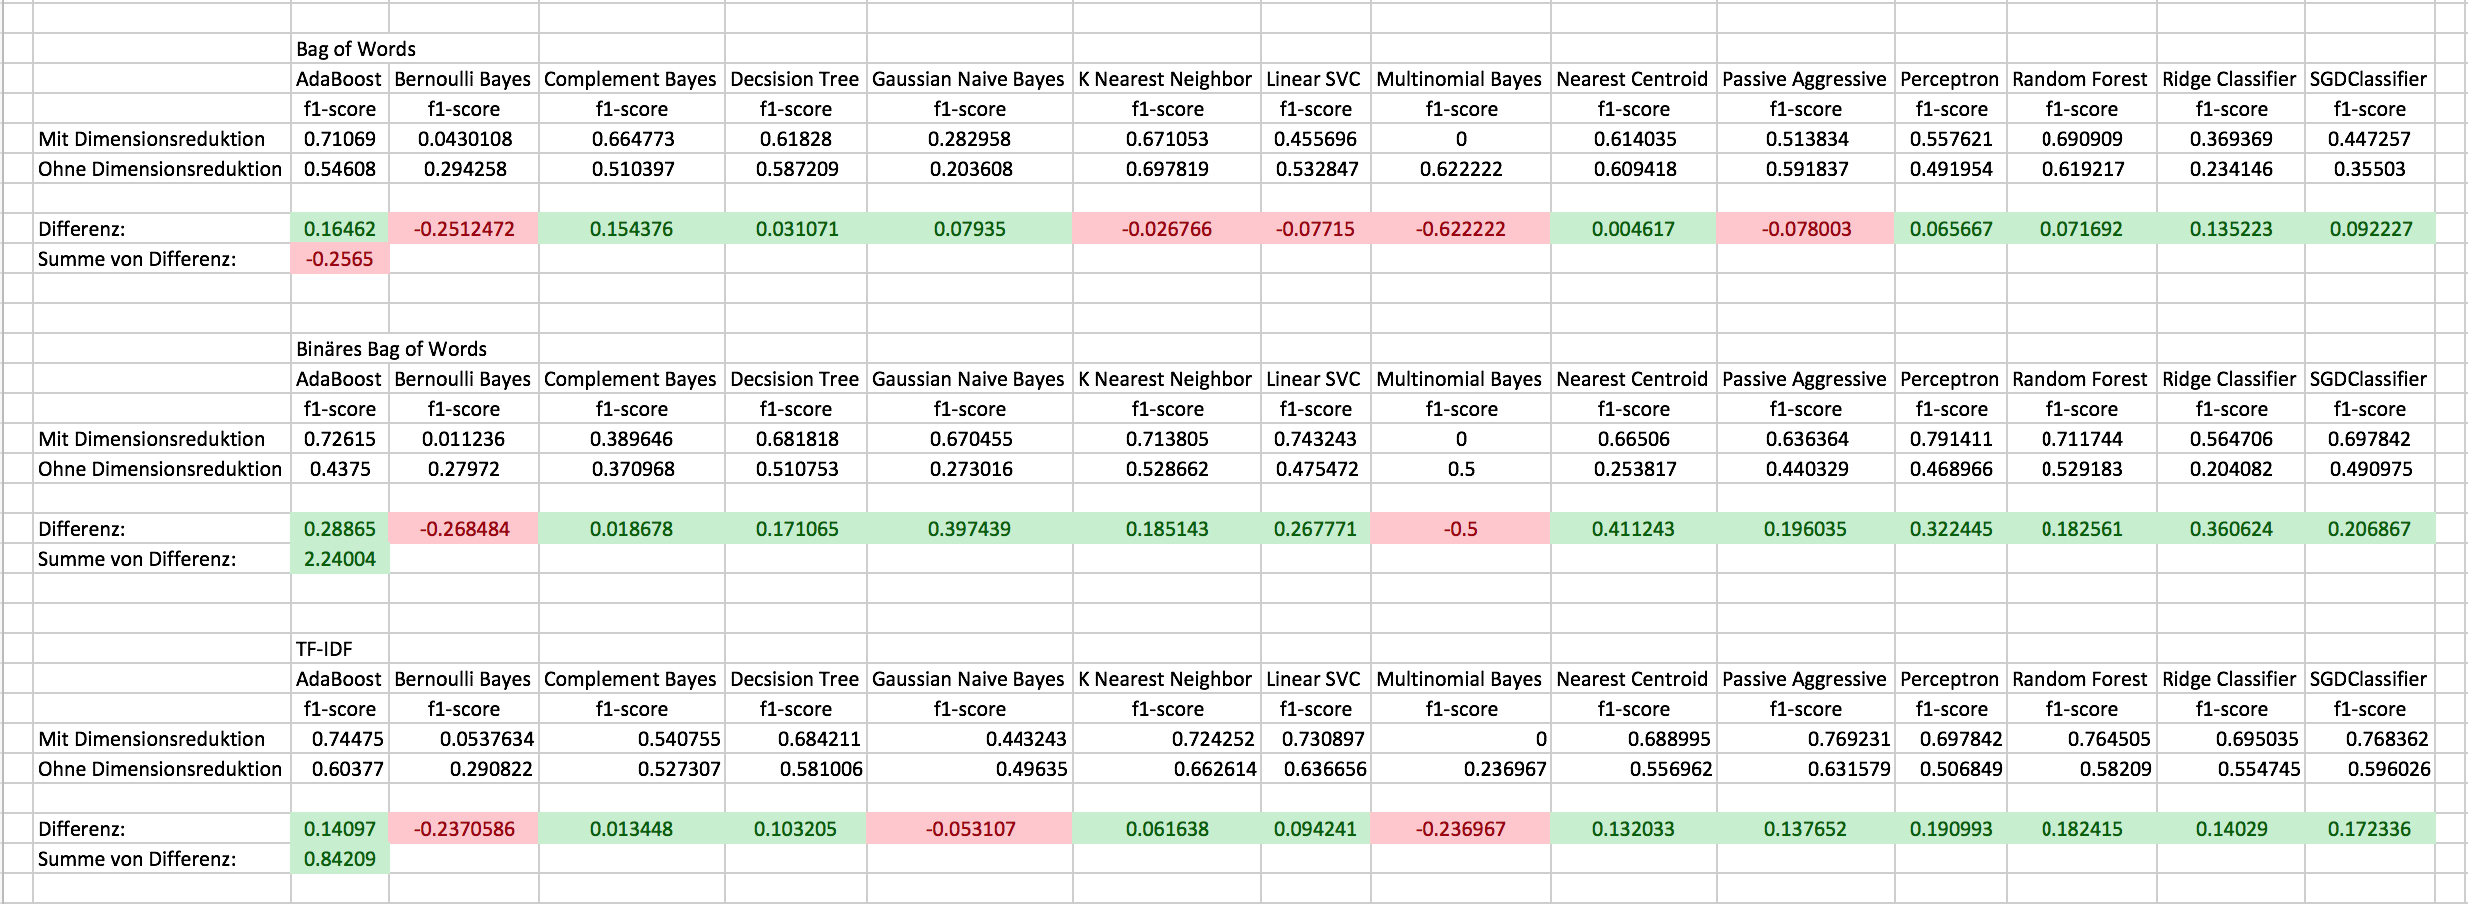
\includegraphics[width=1\columnwidth,keepaspectratio]{img/dimred.png}} 
	\caption{Grafik der Auswertung für die Dimensionsreduktion mittels LSA}
	\source{Eigene Darstellung}
	\label{abb:dimred}
\end{figure}
\subsection{Angabe von Klassenverteilung}
\subsubsection{Methoden}
Da die Daten aus dem Gold Standard eine sehr ungleiche Verteilung von positiven und negativen Samples aufweist, wurde die Klassengewichtung anhand dieser Verteilung berechnet.
Die Gewichtung, auf ein positives Sample folgen 10.32 negative Samples, wurde den Algorithmen fürs Trainieren mitgegeben.
Mittels der Klassenverteilung können die Algorithmen die unterrepräsentierten Klassen, in diesem Falle die positive Klasse, stärker gewichten und den Fokus darauf setzen.
Die Algorithmen wurden mit und ohne Klassengewichtung trainiert und validiert.
Zu erwähnen ist, dass die Gewichtung nicht allen Algorithmen zugewiesen werden konnte, da manche Algorithmen während dem Training solche Informationen nicht verwerten können.
\subsubsection{Resultate}
Die Angabe der Klassenverteilung konnte nicht bei allen Algorithmen als Parameter angegeben werden.
Somit werden alle Bayes-Algorithmen, KNearestNeighbor und Nearest-Centroid in der \cref{abb:classweight} nicht beachtet, da es dort zu keiner Veränderung der Scores kommt.\\
Bei beiden \glqq Bag of Words\grqq{} Methoden erzielt die Angabe der Klassenverteilung eine durchschnittliche Verbesserung der F1-Scores.
Einzelne Algorithmen reagieren negativ auf die Angabe, aber die positiven Auswirkungen übertreffen die negativen Auswirkungen.
Somit wird bei beiden \glqq Bag of Words\grqq{} Methoden die Angabe der Klassenverteilung miteinbezogen.\\
Bei der TF-IDF-Methode werden drei Algorithmen negativ und vier Algorithmen positiv beeinflusst.
Lediglich beim PassiveAgressiveClassifier gibt es eine markante Verschlechterung des F1-Scores.
Bei den anderen Algorithmen halten sich die negativen Auswirkungen im Rahmen.
Den F1-Score des PassiveAgressiveClassifier ausgenommen, sind die positiven Auswirkungen grösser als die negativen Auswirkungen.
Somit wird für TF-IDF ebenfalls die Angabe der Klassenverteilung für die nächsten Schritte beibehalten.
\begin{figure}[H]	
	\centering
	\setlength{\fboxsep}{0.3pt} 
	\setlength{\fboxrule}{0.3pt} 
	\fbox{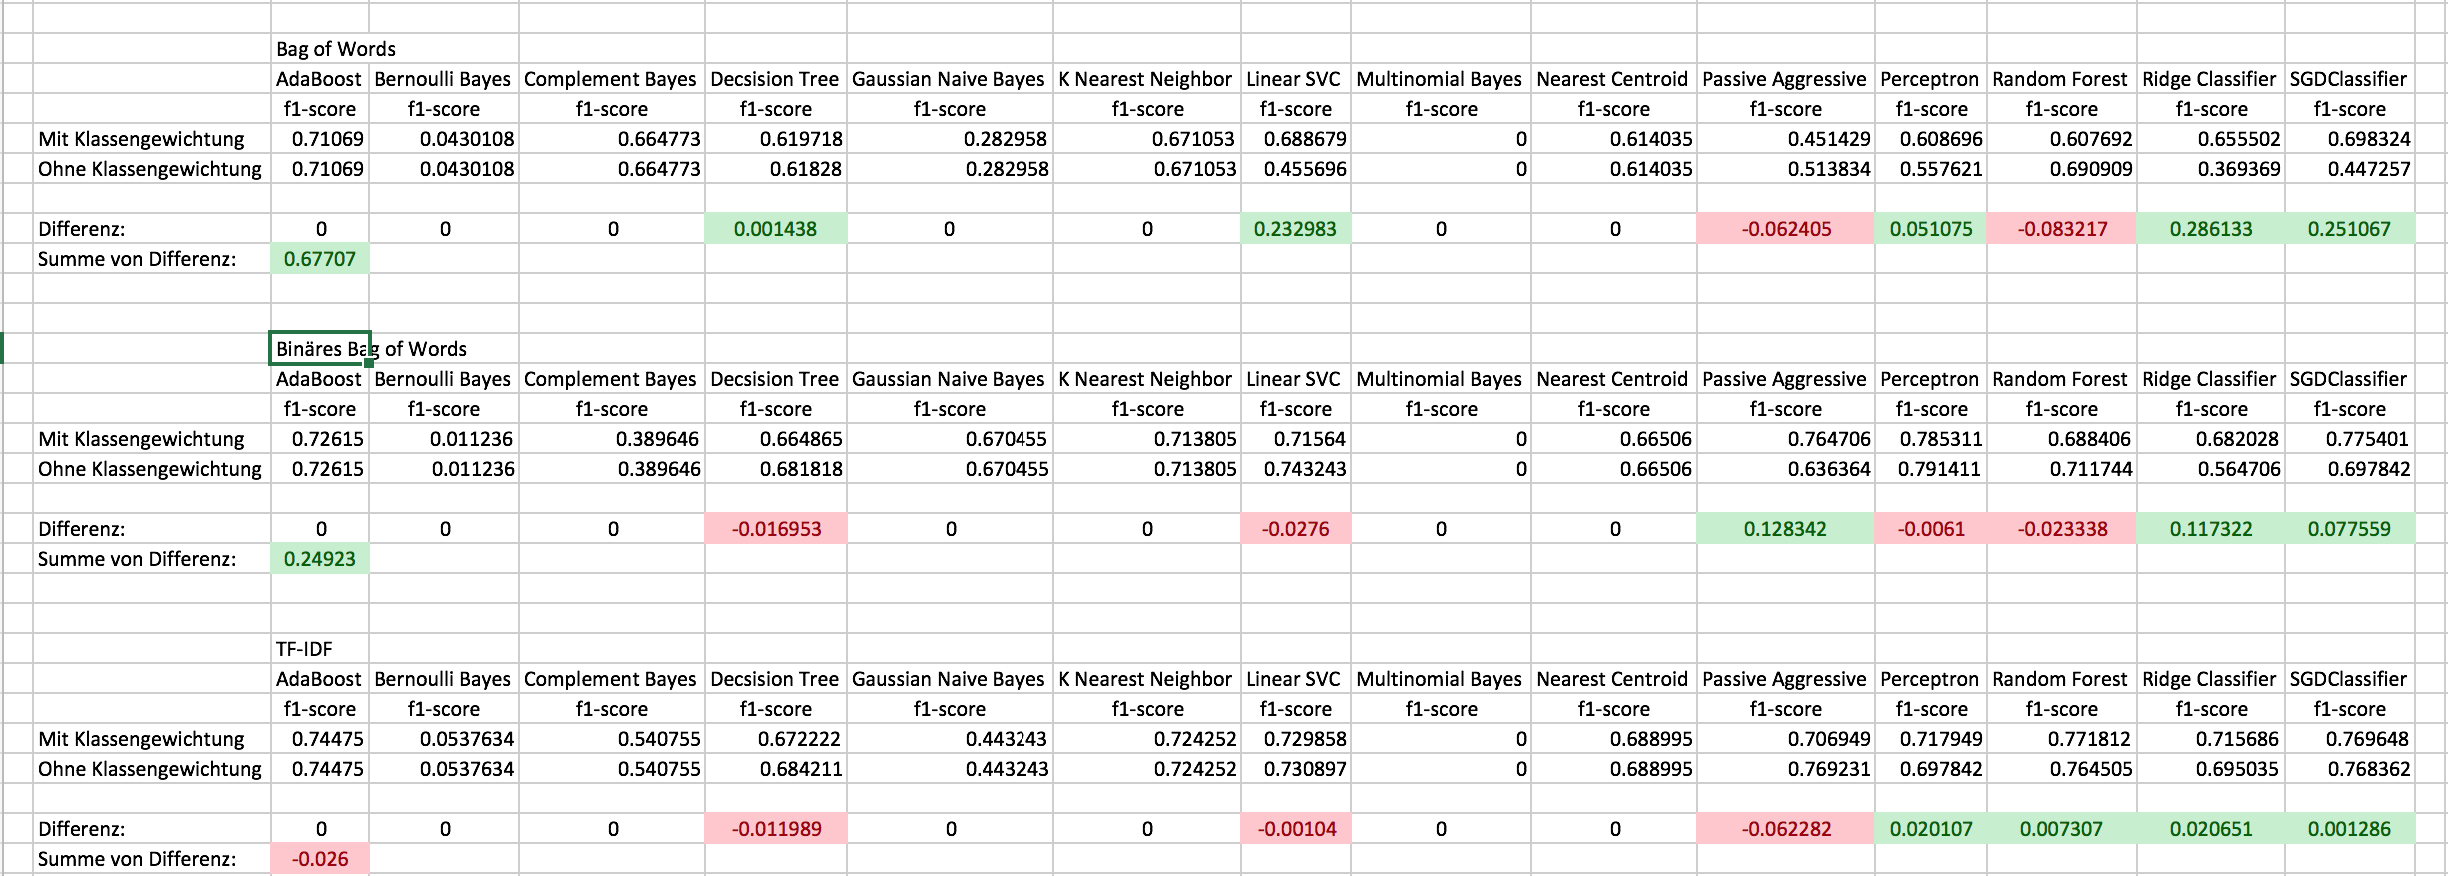
\includegraphics[width=1\columnwidth,keepaspectratio]{img/classweight.png}} 
	\caption{Grafik der Auswertung für die Klassenverteilung}
	\source{Eigene Darstellung}
	\label{abb:classweight}
\end{figure}
\subsection{Anwendung von N-Grammen}
\subsubsection{Methoden}
Die verwendeten Feature-Extraction Methoden bieten die Möglichkeit N-Gramme als Features zu extrahieren.
Aufgrund der Annahme der Autoren, dass verschiedene Menünamen oder Gerichtbezeichnungen in Form von Bi- oder Trigrammen auftreten (Cordon-Bleu, Prosciutto e Funghi), macht die Überprüfung von Bi- und Trigrammen Sinn.\\
Die Scikit-Learn Feature-Extraction Methoden bieten einfache Schnittstellen für die Extrahierung von N-Grammen.
Die Validierung von Uni-, Bi- und Trigrammen wurde für alle drei Feature-Extraction Methoden durchgeführt, die Algorithmen mit den neuen Features trainiert und wieder validiert.
\subsubsection{Resultate}
Die Ergebnisse sind in der \cref{abb:ngram} ersichtlich.
Bei beiden \glqq Bag of Words\grqq{} Methoden erzielt die Verwendung von Unigrammen die besten Ergebnisse.
Bi- und Trigramme können bei einzelnen Algorithmen ebenfalls eine Verbesserunge verzeichnen, aber im Vergleich zu Unigrammen fallen diese flächendeckend kleiner aus.
Somit werden bei beiden \glqq Bag of Words\grqq{} Varianten nur Unigramme verwendet.
Ebenfalls benötigt die Extrahierung der Features bei Bi- und Trigrammen etwa doppelt so lange, was eine enorme Performanceeinbusse ist.\\
Bei der TF-IDF-Methode erzielen Bi- und Trigramme die exakt gleichen Werte.
Dies ist zu erklären, da die TF-IDF Methode keine relevanten Trigramme gefunden hat und somit auf Bigramme zurückgegriffen hat.
Unigramme erzielen im Durchschnitt leicht bessere Werte im Vergleich zu Bi- und Trigrammen.
Jedoch sind von den fünf besten Ergebnissen drei mit Bi-, beziehungsweise Trigrammen erzielt worden, was anhand der gelb markierten Zellen ersichtlich ist.
Da die Entscheidung bei der TF-IDF Methode nicht eindeutig gefällt werden konnte, entschieden sich die Autoren für die Anwendung von Bigrammen.
\begin{figure}[H]	
	\centering
	\setlength{\fboxsep}{0.3pt} 
	\setlength{\fboxrule}{0.3pt} 
	\fbox{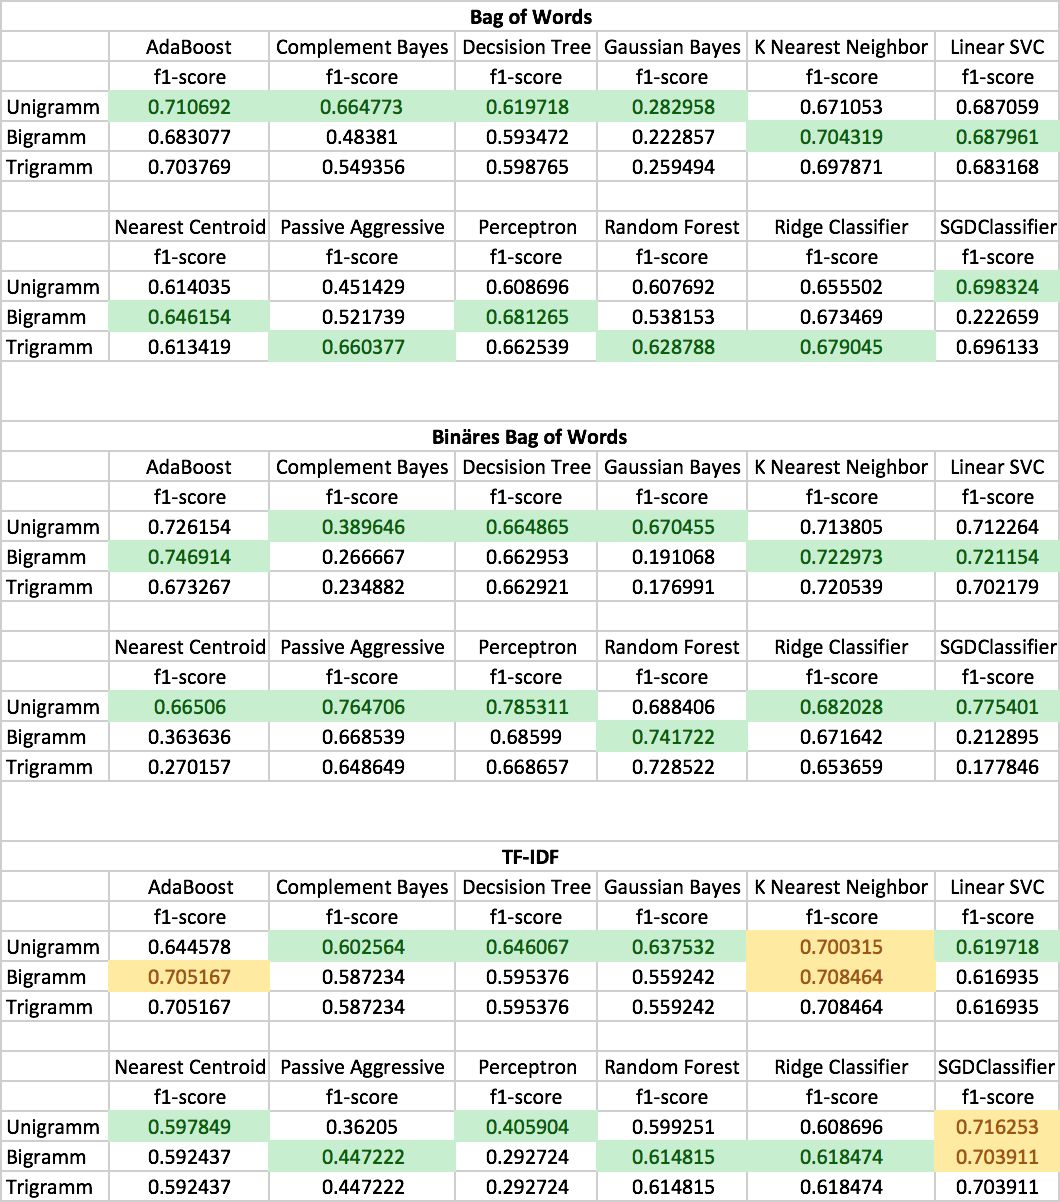
\includegraphics[width=1\columnwidth,keepaspectratio]{img/ngram.png}} 
	\caption{Auswertung der N-Gramme }
	\source{Eigene Darstellung}
	\label{abb:ngram}
\end{figure}
\subsection{Anwendung von fortgeschrittenen Preprocessingschritten}
\subsubsection{Methoden}
Fortgeschrittene Preprocessing-Schritte haben die Aufgabe den Text weiter zu modifizieren und die Extrahierung von zusätzlichen Informationen zu vereinfachen.
Im Kontext vom Machine-Learning Teil zählen folgende Preprocessingschritte zu den fortgeschrittenen Funktionen:
\begin{itemize}
	\item Das Markieren von Preisen mit entsprechenden Tags
	\item Die Stammformreduktion
	\item Das Entfernen von Stopwörtern
	\item Das Markieren von Information, die sich auf Getränke beziehen
\end{itemize}
Diese fortgeschrittenen Funktionen können ebenfalls im Unterkapitel \ref{sec:advancedpre} nachgelesen werden.
Es wurden die Auswirkungen von jeglichen Kombinationen der fortgeschrittenen Preprocessing-Schritten getestet.
Bei vier verschiedenen Arten ergeben sich 16 verschiedene Kombinationen.
\subsubsection{Resultate}
Das fortschrittliche Preprocessing erzielt bei allen drei Feature-Extraction Methoden keine eindeutigen Resultate.\\
Bei der \glqq Bag of Words\grqq{} Methode erreicht die Konfiguration \glqq config8\grqq{} mit dem Preisdetektor, der Stoppwörterentfernung und der Stammformreduktion die grössten positiven Einwirkungen.
Sieben Algorithmen können mit dieser Konfiguration ihre F1-Scores verbessern.
Somit wird für \glqq Bag of Words\grqq{} die Konfiguration \glqq config8\grqq{} weiter benutzt.\\
Bei der binären \glqq Bag of Words\grqq{} Methode gibt es bei keiner Konfiguration irgendwelche flächendeckenden Verbesserungen.
Es gibt jeweils nur vereinzelte Algorithmen, welche ihre Scores verbessern können.
Da keine Konfiguration eindeutig als Verbesserung angesehen werden kann, wird bei dieser Variante keine der fortgeschrittenen Preprocessing-Schritte angewendet.\\
Bei der TF-IDF-Methode gibt es ebenfalls keine eindeutigen Verbesserungen bei irgendeiner Konfiguration.
Es können vereinzelte Algorithmen ihre Scores verbessern, aber es findet nie flächendeckend eine Verbesserung statt.
Bei der Konfiguration \glqq config5\grqq{} erzielt AdaBoost den höchsten Wert über alle Konfigurationen gesehen, aber die anderen Algorithmen werden nur leicht beeinflusst.
Um bei der weiteren Ermittlung von Optimierungen nicht nur auf einen Algorithmus zu setzen, wird bei TF-IDF kein fortgeschrittenes Preprocessing angewendet.
\\\\
Die Auswertung für das fortschrittliche Preprocessing kann im Anhang \cref{app:electronic} im Zip-Ordner mit den Log- und Konfigurationsdateien gefunden werden.
\subsection{Anzahl Features}
\subsubsection{Methoden}
Jeder Algorithmus verhaltet sich mit der Änderung der Anzahl extrahierter und dimensionsreduzierter Features unterschiedlich.
Um eine optimale Anzahl an Features zu ermitteln, wurde die Anzahl Features schrittweise erhöht , die Algorithmen mit der neuen Anzahl trainiert und schlussendlich validiert.
Dies ist ein rechenintensives Unterfangen, führt in der Regel jedoch zu spürbaren Verbesserungen der Scores bei allen Algorithmen.
Die Messungen wurden mit einer Anzahl Features von 10 gestartet und schrittweise um 25 Features erhöht, bis schlussendlich eine maximale Anzahl von 400 Features erreicht wurde.
Da die Rechenzeit stetig mit der Erhöhung der Features steigt, wurde die Grenze bei 400 Features gesetzt.
Grundsätzlich macht eine Begrenzung der Features Sinn, da ab einer gewissen Anzahl Features die Algorithmen mit der Handhabung der Features überfordert sind und dies sich dementsprechend auf schlechteren Scores widerspiegelt.
\subsubsection{Resultate}
Für alle drei Feature-Extraction Methoden wurde ein Liniendiagramm für F1-Score, Precision und Recall erstellt.
Aus diesen Grafiken kann entnommen werden, bei welcher Feature-Anzahl welcher Algorithmus den besten Score erzielt.
Für die weitere Auswertung ist die Grafik für F1-Score massgebend und wird weiter analysiert.\\

\textbf{Bag of Words}\\
In der \cref{abb:bow-f1} ist ersichtlich, dass mit \glqq Bag of Words\grqq{} der Algorithmus AdaBoost bei 100 Features mit Abstand den besten F1-Score erzielt und fast die 0.8 Marke erreicht.
Ebenfalls kann der LinearSVC Algorithmus einen guten F1-Score erzielen und teilt sich mit AdaBoost die besten Werte.
Ersichtlich ist ebenfalls, dass die meisten Algorithmen sich zwischen 0.6 und 0.7 bewegen und das vereinzelte Klassifizierer mit ihren Werten auf und ab springen.\\
Die springenden Algorithmen Perceptron, SGDClassifier und PassiveAgressiveClassifier sind alle von der Familie \glqq Linear\_Model\grqq{}. Ein Grund für das auffällige Verhalten wurde nicht gefunden.
\begin{figure}[H]
	\centering	
	\setlength{\fboxsep}{0.3pt} 
	\setlength{\fboxrule}{0.3pt} 
	\fbox{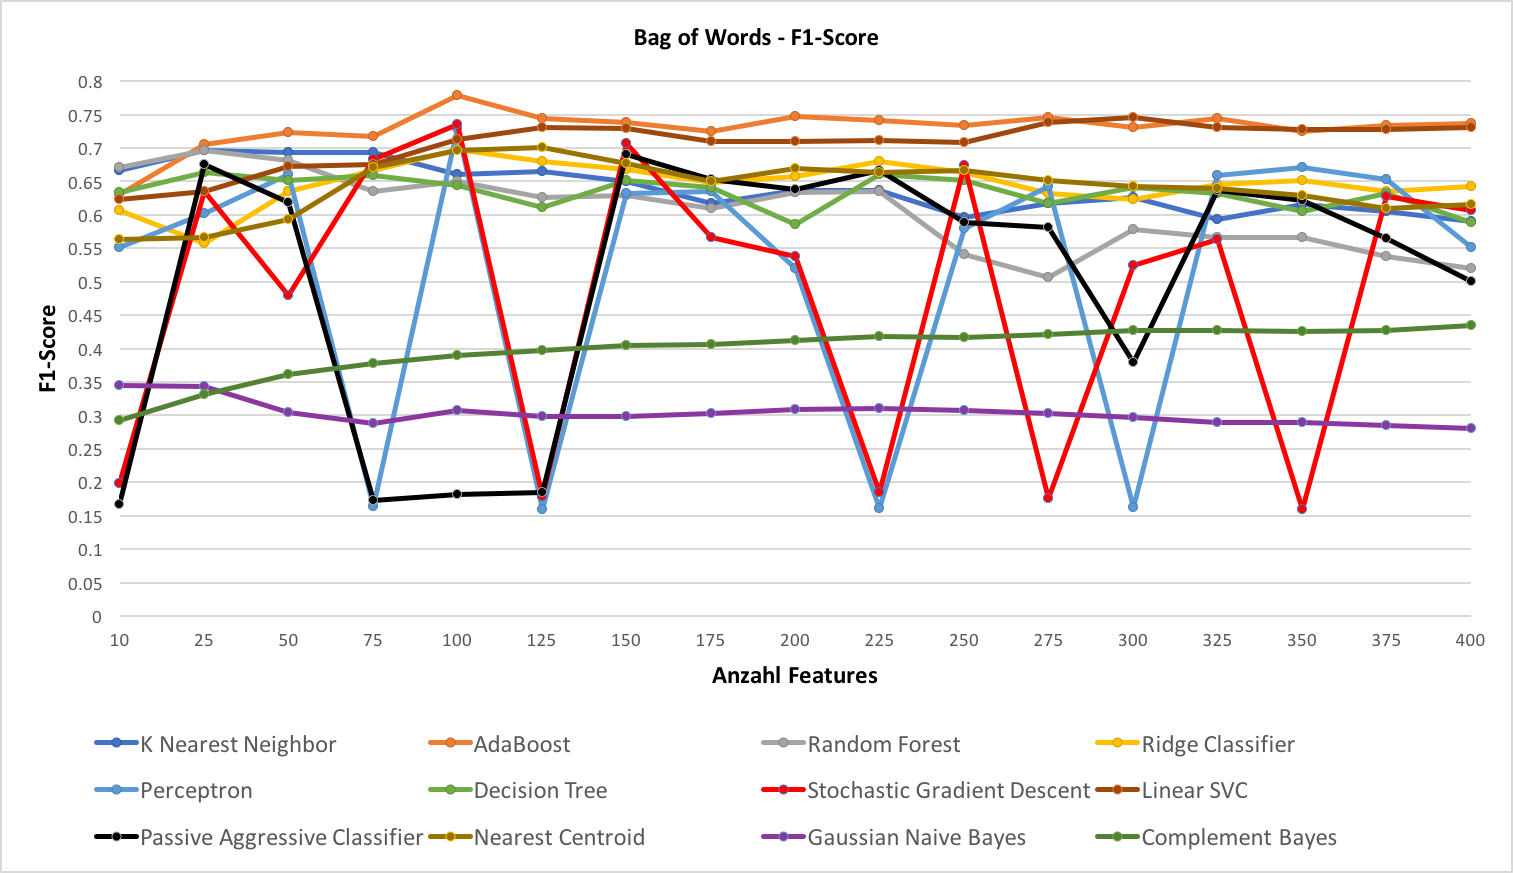
\includegraphics[width=1\columnwidth,keepaspectratio]{img/bow-f1.png}} 
	\caption{Grafik des F1-Score-Verlaufs bei Bag of Words}
	\source{Eigene Darstellung}
	\label{abb:bow-f1}
\end{figure}

\textbf{Binäres Bag of Words}\\
Bei der Methode \glqq binäres Bag of Words\grqq{} können mehrere Algorithmen einen F1-Score nahe der 0.8 Grenze verbuchen.
In der \cref{abb:bow-bin-f1} ist klar erkennbar, dass die meisten Algorithmen einen F1-Score zwischen 0.6 und 0.8 erzielen.
Der beste Algorithmus ist Perceptron, welcher mit 325 Features einen F1-Score von 0.8 verzeichnet.\\
Der SGDClassifier erreicht ebenfalls einen F1-Score von 0.8, jedoch mit einer höheren Anzahl von Features.
Dies bedeutet das SGDClassifier potenziell länger für die Feature-Extraction benötigt und somit ist Perceptron der favorisierende Algorithmus bei dieser Variante.\\
Die Sprünge der linearen Modelle, welche bereits bei der oberen \glqq Bag of Words\grqq{} Methode dargestellt wurden, sind ebenfalls wieder in der F1-Score-Grafik \cref{abb:bow-bin-f1} zu erkennen.
\begin{figure}[H]
	\centering	
	\setlength{\fboxsep}{0.3pt} 
	\setlength{\fboxrule}{0.3pt} 
	\fbox{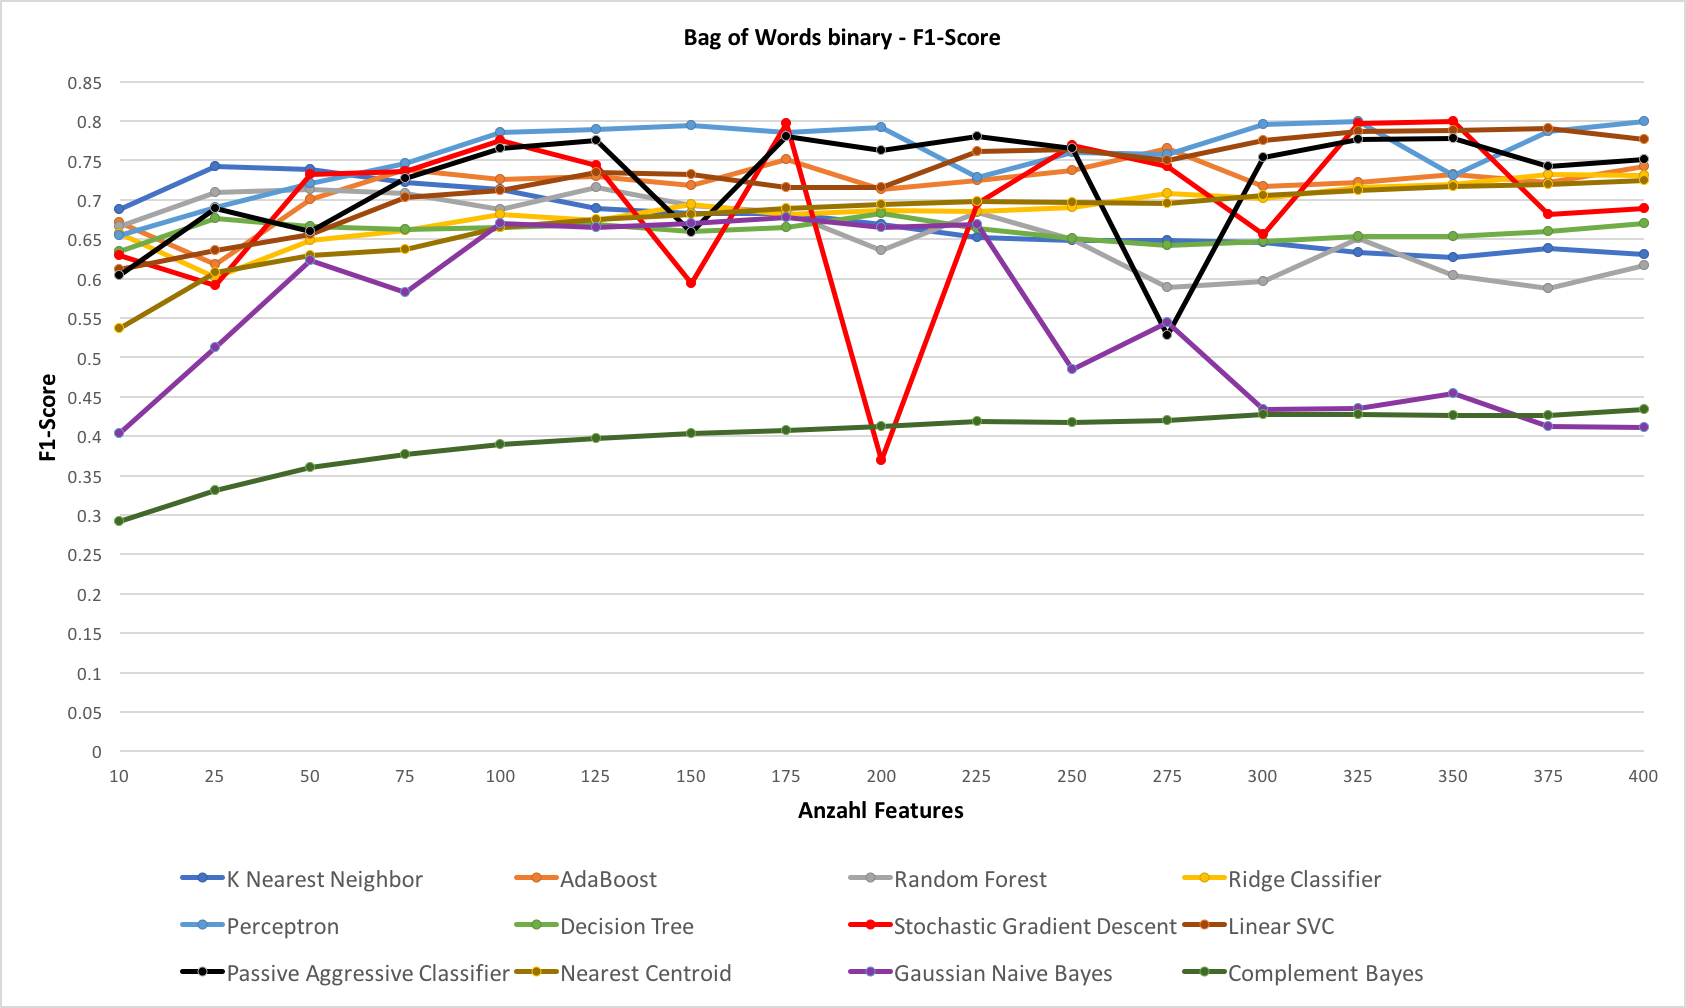
\includegraphics[width=1\columnwidth,keepaspectratio]{img/bow-bin-f1.png}} 
	\caption{Grafik des F1-Score-Verlaufs bei binärem Bag of Words}
	\source{Eigene Darstellung}
	\label{abb:bow-bin-f1}
\end{figure}

\textbf{TF-IDF}\\
Bei der Verwendung von TF-IDF sind mehrere Algorithmen mit ihren F1-Scores im Bereich 0.7 bis 0.8.
In der \cref{abb:tfidf-f1} ist erkennbar, dass der SGDClassifier Algorithmus als einziger die Grenze von 0.8 durchbrechen kann.
Dies erreicht er mit einer Anzahl Features von 150 und ist somit der Algorithmus mit dem besten F1-Score.\\
Auch bei der TF-IDF Methode sind wieder Sprünge bei den linearen Modellen in der F1-Score-Grafik \cref{abb:tfidf-f1} deutlich erkennbar.
\begin{figure}[H]	
	\centering
	\setlength{\fboxsep}{0.3pt} 
	\setlength{\fboxrule}{0.3pt} 
	\fbox{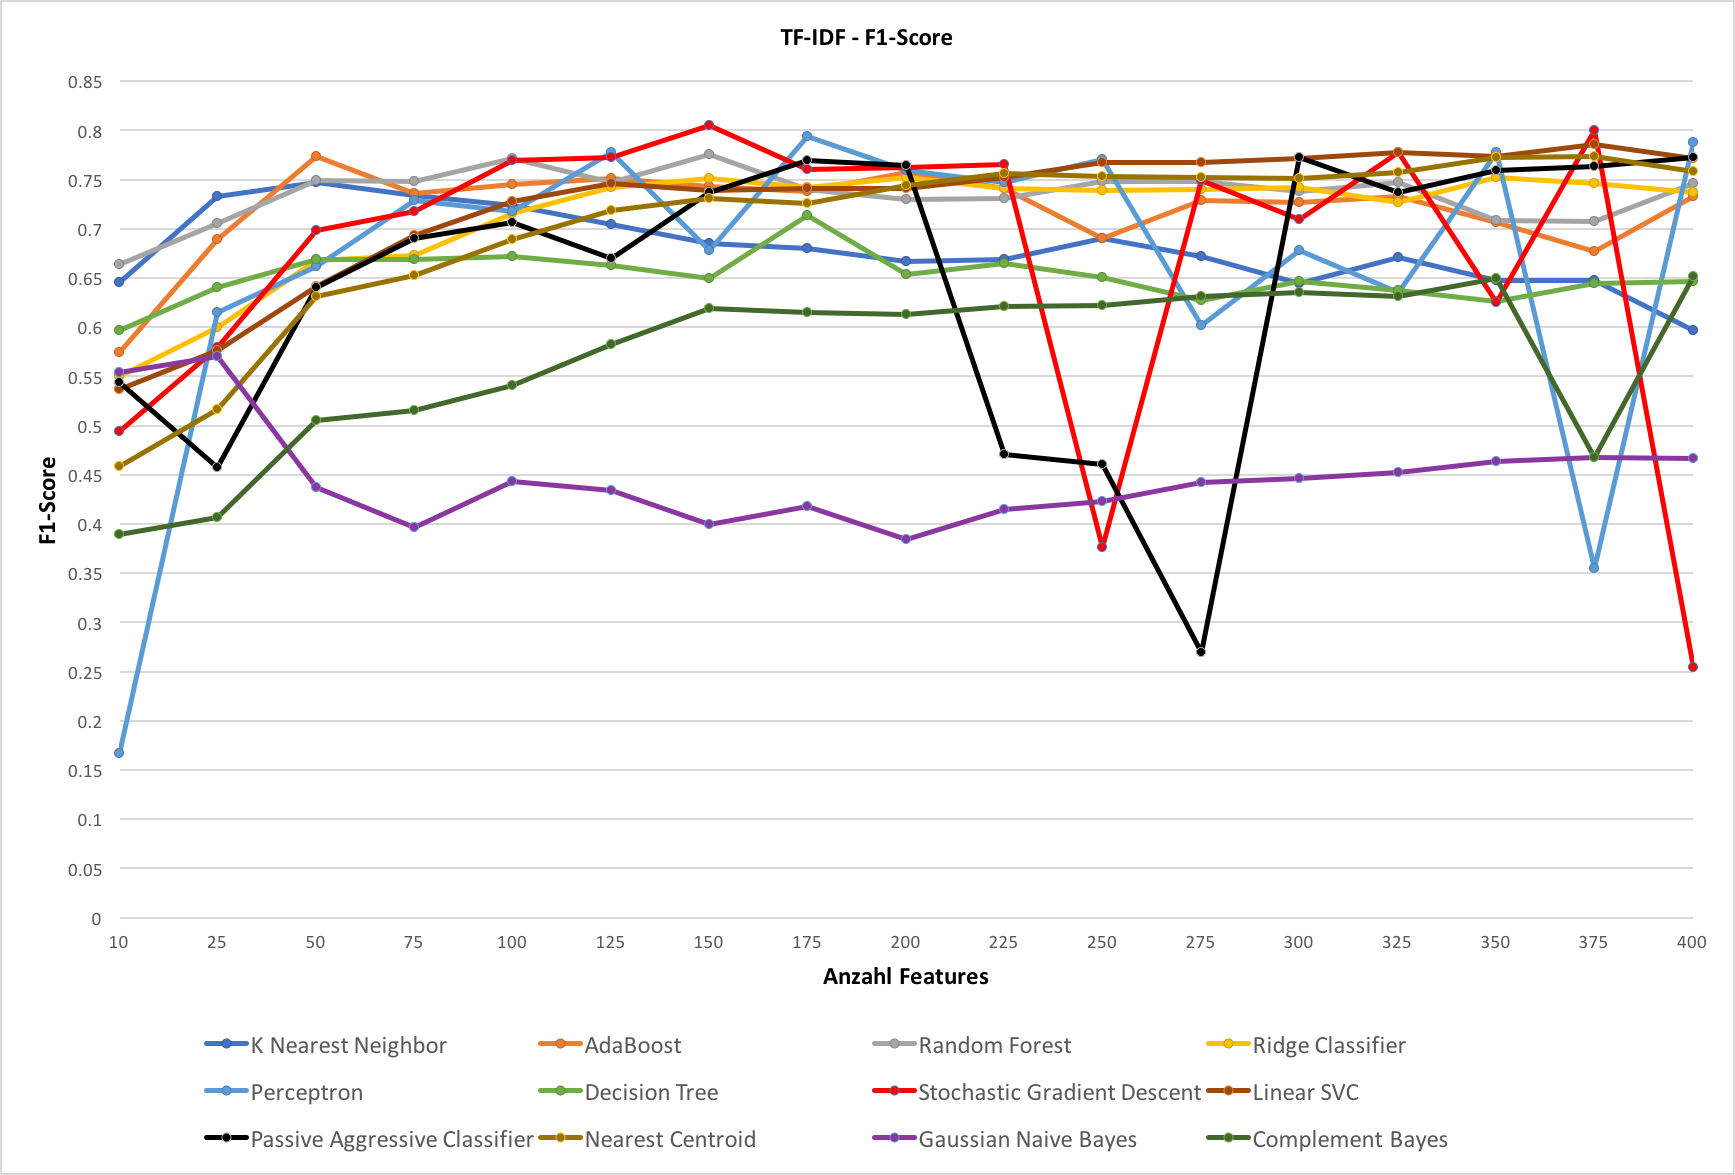
\includegraphics[width=1\columnwidth,keepaspectratio]{img/tfidf-f1.png}} 
	\caption{Grafik des F1-Score-Verlaufs bei TF-IDF}
	\source{Eigene Darstellung}
	\label{abb:tfidf-f1}
\end{figure}
\subsection{Hyperparametertuning}
\subsubsection{Methoden}
Als letzter Schritt der Algorithmenoptimierung wurde eine ausführliche Hyperparametersuche inklusive Kreuzvalidierung mit einem Wert von fünf durchgeführt.
Es wurden für die drei Feature-Extraction Methoden jeweils das Modell mit dem besten F1-Score kreuzvalidiert.
Für jedes Modell wurde eine Liste von anpassbaren Parametern zusammengestellt, welche Scikit-Learn vorgibt.
Für jeden Parameter wurde ein Bereich von möglichen Werten angegeben.
Mittels der Funktion \glqq GridSearchCV\grqq{}\footnote{\url{https://scikit-learn.org/stable/modules/generated/sklearn.model_selection.GridSearchCV.html}abgerufen am: 07.05.2019} von Scikit-Learn wurde die Hyperparametersuche für die Optimierung des F1-Scores durchgeführt.\\
Je nach Algorithmus und Grösse der Parameterliste kann die Hyperparametersuche sehr lange dauern.
Ebenfalls ist es möglich, dass die Standardparameter bereits ein Optimum darstellen und keine besseren Parameter gefunden werden.
\subsubsection{Resultate}
Die drei Modelle, welche aus dem vorherigen Experiment als die besten entnommen wurden, werden mittels Kreuzvalidierung auf optimale Hyperparameter durchsucht.\\
Die drei Modelle AdaBoost, SGDClassifier und Perceptron konnten die besten F1-Scores erzielen.\\
\begin{table}[H]
	
	\centering
	\label{tab:ada}
	\begin{tabular}{|l|l|l|l|}
		\hline
		& F1-Score & Precision & Recall\\
		\hline
		Vor Hyperparametertuning & 0.778 & 0.837 & 0.727 \\
		Nach Hyperparametertuning & 0.788 & 0.817 & 0.761 \\
		\hline
	\end{tabular}
	\caption{Auwertung Hyperparametertuning für AdaBoost mit binärem Bag of Words}
\end{table}
\begin{table}[H]
	\centering
	\label{tab:per}
	\begin{tabular}{|l|l|l|l|}
		\hline
		& F1-Score & Precision & Recall\\
		\hline
		Vor Hyperparametertuning & 0.8 & 0.872 & 0.739 \\
		Nach Hyperparametertuning & 0.579 & 0.426 & 0.903 \\
		\hline
	\end{tabular}
	\caption{Auwertung Hyperparametertuning für Perceptron mit Bag of Words}
\end{table}
\begin{table}[H]
	\centering
	\label{tab:sgd}
	\begin{tabular}{|l|l|l|l|}
		\hline
		& F1-Score & Precision & Recall\\
		\hline
		Vor Hyperparametertuning & 0.805 & 0.768 & 0.847 \\
		Nach Hyperparametertuning & 0.762 & 0.682 & 0.864 \\
		\hline
	\end{tabular}
	\caption{Auwertung Hyperparametertuning für SGDClassifier mit TF-IDF}
\end{table}
In der \cref{tab:ada} ist auffällig, dass AdaBoost als einziges Modell bessere Hyperparameter mittels Hyperparametertuning finden konnte.\\
AdaBoost kann seinen Recall verbessern, gleichzeitig verschlechtert sich aber seine Precision.
Da die Recallsteigerung grösser als der Precisionabfall ist, wird der F1-Score nach oben korrigiert.\\
Die anderen beiden Modelle Perceptron in \cref{tab:per} und SGDClassifier in \cref{tab:sgd} erzielen mit den neuen Parametern schlechtere Werte.
Beide können den Recall verbessern, jedoch müssen sie massive Gefälle bei der Precision einbüssen.
Da die Precision viel stärker abgenommen, als der Recall zugenommen hat, wird der F1-Score schlechter.\\
Somit sind die Standardparameter für Perceptron und SGDClassifier für den \glqq Use-Case: Restaurant-Suchmaschine\grqq{} bereits optimal gewählt worden, da beim Hyperparametertuning eine ausführliche Liste von veränderbaren Parametern keine Verbesserung erzielen konnte.\\
Perceptron hat im Vergleich zum SGDClassifier einen leicht tieferen F1-Score, jedoch ist seine Precision deutlich höher.
Da für den schlussendlichen \glqq Use-Case\grqq{} Precision wichtig ist, wird das Perceptron-Modell für weitere Auswertungen verwendet.
Die Annahme der Autoren lautet, dass es bei einer Suchmaschine wichtiger ist, richtige Ergebnisse anstatt möglichst viele Ergebnisse zu finden.
Aufgrund dieser Annahme wird das Perceptron-Modell für eine produktive Pipeline weiterverwendet.

\section{Diskussion}
Die Resultate der Experimente der zwei verschiedenen Ansätze anhand der Testdaten zeigen, dass mit regelbasierten Methoden ein fast gleich guter Score erreichbar ist wie mit Machine-Learning.
Beide Ansätze erzielen eine hohe Precision.
Es ist jedoch zu berücksichtigen, dass die Resultate der regelbasierten Methode bei steigender Anzahl Daten schlechter werden.

\subsection{Diskussion der Resultate der regelbasierten Experimente}
Der Regelsatz \glqq Menü im Titel\grqq{} hat im Bezug auf den F1-Score das schlechteste Ergebnis geliefert, dafür einen Precision-Wert von 1.
Es ist also keine Webpage fälschlicherweise als Menüseite klassifiziert worden.
Dafür wurden nur 16\% der Menüseiten erkannt.

Die Suche nach Preisen innerhalb des Textes hat ein besseres Ergebnis geliefert, 50\% der Menüseiten wurden als solche erkannt und zwei Webpages wurden fälschlicherweise als Menüseiten klassifiziert. 
Eine Kombination dieser beiden Methoden ergibt eine fast identische Klassifikation.
28 von 50 Menüseiten wurden erkannt, ebenfalls zwei wurden fälschlicherweise als Menüseiten klassifiziert.

Durch das Verwenden einer Blacklist und Whitelist wurden fast gleich viele Menüseiten korrekt erkannt. Bei 26, also ca. 52\% der erkannten Webseiten wurde nur eine Webpage als Menüseite klassifiziert, welche keine ist.

Die Klassifikation mit der Methode \glqq Bag of Words\grqq{} führt zu den besten Ergebnissen der regelbasierten Klassifikation.
31 von 50 Menüseiten wurden erkannt, zudem wurden 3 Webpages fälschlicherweise als Menüseiten klassifiziert.\\

Alle Methoden erreichten auf dem Testdatensatz eine hohe Precision, jedoch ist der Recall jeweils so tief, dass der F1-Score nicht die vorausgesetzte Marke von 0.8 überschreitet.
Alle Methoden der regelbasierten Klassifikation mit Ausnahme der Methode \glqq Bag of Words\grqq{} funktionieren unabhängig vom Trainingsdatensatz.
Beim Evaluieren der besten Konfigurationsparameter wurden diese auf einem Split des Trainingsdatensatzes (ein sogenanntes Validationsset) getestet.
Im Vergleich zu den Ergebnissen des Testsets ist bei allen Regeln zu erkennen, dass die Werte deutlich tiefer sind.
Daraus kann die Schlussfolgerung gezogen werden, dass mit einer steigenden Anzahl zu klassifizierenden Daten die Diversität dieser steigt, was sich negativ auf die Ergebnisse auswirkt.
Insgesamt ist zu erkennen, dass eine qualitativ und quantitativ hochwertige Klassifikation von Webpages mit einem regelbasierten Ansatz vor allem mit steigender Datendiversität nicht möglich ist.
In allen Fällen wurde eine erhebliche Anzahl der Menüseiten nicht gefunden.
Wenn man dies nun auf den Anwendungsfall einer Suchmaschine überträgt, werden viele Menüseiten nicht angezeigt.
Im Bezug auf die Resultate des Trainingsdatensatzes ist zudem die Precision markant gesunken.
Dadurch werden im Anwendungsfall viele Webpages angezeigt, welche keine Menüseiten sind.
\subsection{Diskussion der Experimente mittels Machine-Learning}
Bei allen Experimenten wurden die Modelle jeweils auf dem Validierungsset validiert.
Um nun die wirkliche Performance des besten Modells zu überprüfen, wird die Klassifizierung mit dem ungesehenen Testset durchgeführt.
Für die Auswertung werden der F1-Score, die Precision und der Recall aufgezeigt.
Zusätzlich wird eine Konfusionsmatrix erstellt, welche darlegt, wie viele Webpages korrekt oder falsch eingestuft worden sind.
\\\\
Hinweis: Beim Perceptron wurde bei der Hyperparametersuche keine besseren Parameter gefunden.
Aufgrund dessen wurden die Standardparameter weiter verwendet.

\begin{table}[H]
	\centering
	\label{tab:bestclf}
	\begin{tabular}{|l|l|l|l|}
		\hline
		Methode & F1-Score & Precision & Recall\\
		\hline
		Perceptron mit binärem Bag of Words & 0.78 & 0.92 & 0.68 \\
		\hline
	\end{tabular}
	\caption{Bester Algorithmus der Machine-Learning Klassifikation}
\end{table}

\begin{table}[H]
	
	\centering
	\label{tab:conf}
	\begin{tabular}{@{}cc|cc@{}}
		\multicolumn{1}{c}{} &\multicolumn{1}{c}{} &\multicolumn{2}{c}{Predicted} \\ 
		\multicolumn{1}{c}{} & 
		\multicolumn{1}{c|}{} & 
		\multicolumn{1}{c}{Positiv} & 
		\multicolumn{1}{c}{Negativ} \\ 
		\cline{2-4}
		\multirow[c]{2}{*}{\rotatebox[origin=tr]{90}{Actual}}
		& Positiv  & 34   & 16   \\[1.5ex]
		& Negativ  & 3   & 47 \\ 
		\cline{2-4}
	\end{tabular}
	\caption{Konfusionsmatrix der Methode: Perceptron mit binärem Bag of Words}
\end{table}
Im \cref{tab:bestclf} ist ersichtlich, dass im Vergleich zum \cref{tab:per} der F1-Score leicht abgenommen hat.
Dies hat den Grund, dass der Recall spürbar an Wert verloren hat.
Die Precision jedoch stieg und wirkte der Reduzierung des F1-Scores entgegen.\\
In der Konfusionsmatrix (\cref{tab:conf}) ist deutlich die hohe Precision zu erkennen.
Der Algorithmus klassifizierte 34 Webpages korrekt als Menüseiten.
Ebenfalls wurden nur drei Webpages als Menüseiten klassifiziert, welche aber keine gewesen sind.
Die schlussendliche Performance des Klassifizierers ist für den genannten \glqq Use-Case\grqq{} zufriedenstellend und somit wird der Algorithmus Perceptron in einer produktiven Pipeline weiterverwendet.
\\\\
Schlussendlich ist ersichtlich, dass die Variante mit dem Perceptron-Algorithmus eine qualitative und quantitative Klassifizierung von Menüseiten erzielen kann.
Der F1-Score liegt zwar leicht unter dem selbst definierten Schwellwert von 0.8, jedoch ist die Precision mit 0.92 weit darüber.\\

Für den Anwendungsfall einer Suchmaschine ist es besser, wenn nicht möglichst viel gefunden wird, sondern dass das Gefundene effektiv korrekt ist.
Dennoch dürfen nicht nur eine Hand voll Menüseiten gefunden werden, damit das Angebot nicht verkümmert.\\
Der Perceptron-Algorithmus bietet einen guten Kompromiss zwischen Precision und Recall und wird deshalb für die Suchmaschine verwendet.
Mit seiner Precision von 0.92 erreicht er bei 37 Vorhersagen nur drei falsche Einschätzungen.
Somit wäre in der Suchmaschine jeder 13. Vorschlag falsch, was nach der Meinung der Autoren vertretbar ist.
\section{Beantwortung der Forschungsfrage}
Unter Verwendung der Daten des Gold Standards und dem selbst vorgegebenen Ziel eines F1-Scores von mindestens 0.8 lautet die Antwort auf die Forschungsfrage:\\
\emph{Nein, Restaurant-Webseiten können mit den erarbeiteten Klassifizierern nicht mit hoher Wahrscheinlichkeit klassifiziert werden, ob sie Menüinformationen beinhalten.}



\newpage

\chapter{Teil 3: Engineering}
\label{chap:engineering}
Dieses Kapitel beinhaltet den praktischen Teil dieser Arbeit.
Die Erarbeitung und die verwendeten Technologien des Webcrawlers sowie der Webapplikation werden genauer erläutert.
\section{Webcrawler}
Der Webcrawler dient zur Erarbeitung der Rohdaten des in \cref{chap:gold_standard} beschriebenen Gold Standards.
Zusätzlich wurden diese Rohdaten mit einem der in \cref{chap:classification} erarbeiteten Algorithmen klassifiziert und als Grundlage für die Daten der Webapplikation verwendet.
\subsection{Stand der Forschung}
Ein Webcrawler ist ein Programm, das automatisch das World Wide Web durchsucht und Webseiten analysiert \cite[p. 311]{liu2007web}.
Ein Webcrawler verwendet als Startpunkt ein Seed, welches URLs enthält.
Der Ablauf, welcher in \cref{fig:flowchart_webcrawler} gezeigt wird, ist wie folgt zu verstehen:
Die URLs aus dem Seed werden in eine Queue, genannt Frontier, geladen.
Von da aus werden diese Webpages aufgerufen und nach weiteren URLs durchsucht.
Die gefundenen URLs werden ebenfalls zum Frontier hinzugefügt, die Webpage selbst wird gespeichert.
Dieser Ablauf findet solange statt bis ein gewisses Ziel erreicht ist. \cite[p. 313]{liu2007web}
\begin{figure}
	\centering
	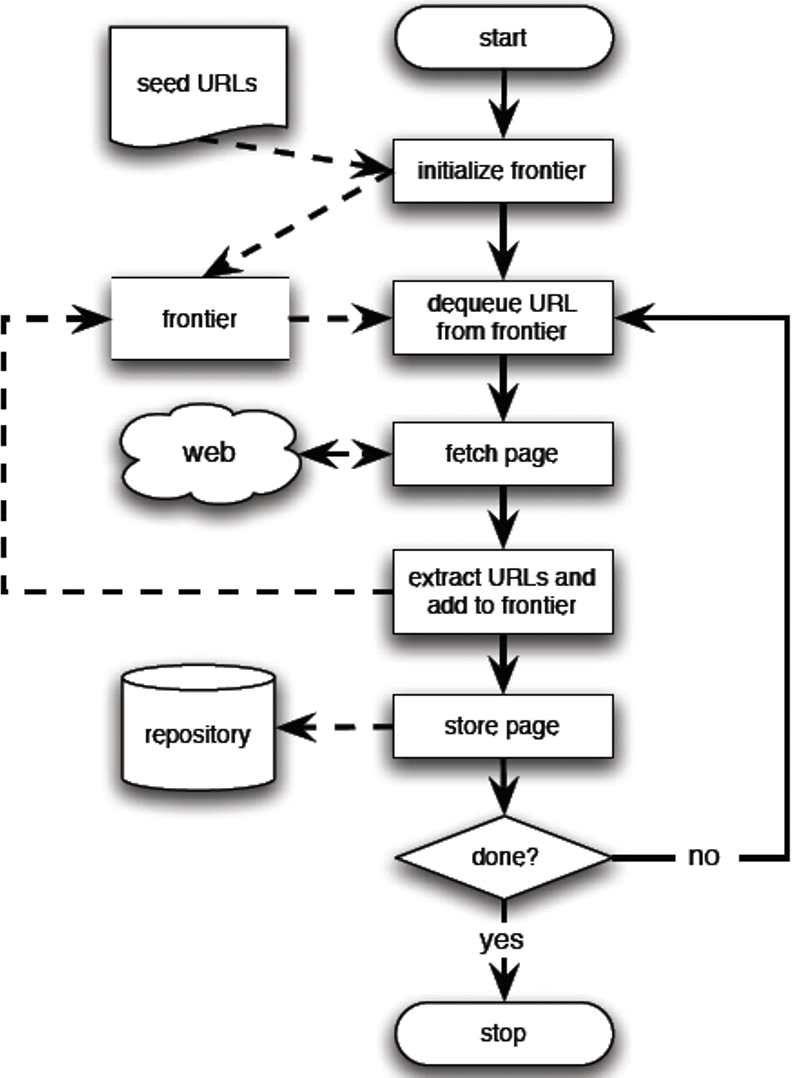
\includegraphics[width=0.8\columnwidth,keepaspectratio]{img/flowchart_webcrawler.png}
	\caption{Ablauf eines Webcrawlers}
	\source{\cite[p. 313]{liu2007web}}
	\label{fig:flowchart_webcrawler}
\end{figure}
\subsection{Evaluation}
Es fand keine Evaluation zur Findung eines geeigneten Webcrawlers statt.
StormCrawler SDK wird eingesetzt, da an der Hochschule für Technik und Wirtschaft Chur ein Team bereits mit diesem arbeitet und dadurch Know-how besitzt.
Dieses Team, speziell ein wissenschaftlicher Mitarbeiter, hat Support angeboten, weshalb die Entscheidung getroffen wurde, StormCrawler SDK zu verwenden.
\FloatBarrier
\subsection{Beschreibung der Technologie und Anpassungen}
Nachfolgend werden die verschiedenen Technologien beschrieben, welche verwendet wurden, um den Webcrawler zu realisieren.
\subsubsection{Apache Storm}
StormCrawler basiert auf Apache Storm, einem Opensource Framework zur verteilten Stream-Verarbeitung.
Die Architektur von Apache Storm basiert auf den folgenden Komponenten:
\begin{itemize}
	\item Spout - Komponente zum Einlesen von Daten-Streams
	\item Bolt - Komponente zum Verarbeiten von Daten-Streams
	\item Tupel - Datensatz, welcher zwischen den Komponenten weitergegeben wird
	\item Topologie - Ein Netz bestehend aus Spouts und Bolts
\end{itemize}
Jede Komponente ist als eigene Java-Klasse definiert und beinhaltet zwingend die folgenden Methoden \footnote{\url{https://dev.to/usamaashraf/playing-with-apache-storm-on-docker---like-a-boss-4bgb} abgerufen am: 08.01.2019}:
\begin{itemize}
	\item declareOutputFields() - Definition des Ausgabeschemas des Tupels
\end{itemize}
Jeder Bolt enthält zudem eine weitere Methode:
\begin{itemize}
	\item execute() - Ausführen des Tasks der Komponente
\end{itemize}
In einer Topologie werden verschiedene Spouts und Bolts miteinander verknüpft, um einen Prozess durchzuführen, wie in \cref{fig:topology} gezeigt wird.
\begin{figure}[H]
	\centering	
	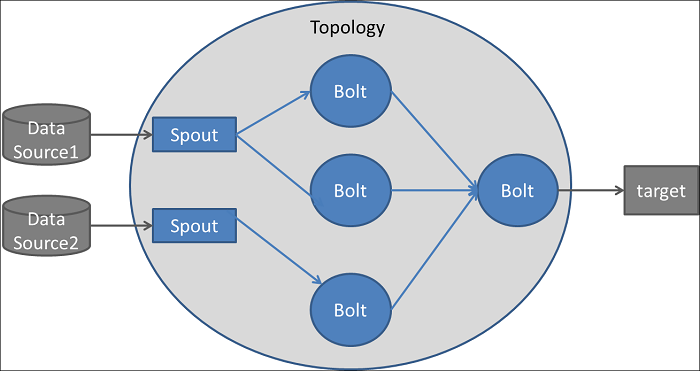
\includegraphics[width=0.8\columnwidth,keepaspectratio]{img/storm-topology.png}
	\caption{Beispieltopologie}
	\source{\url{https://dzone.com/articles/apache-storm-architecture} aufgerufen am 08.01.2019}
	\label{fig:topology}
\end{figure}
Dabei hat der Spout die Aufgabe, Daten aus einer Quelle (z.B. Datei, Datenbank, Array) einzulesen und daraus ein Tupel zu bilden.
Dieses Tupel wird an Bolts der Topologie weitergegeben und von diesen verarbeitet.
Diese Verarbeitung muss nicht seriell stattfinden.
Die Topologie kann auch Gabelungen beinhalten, die dementsprechend Bolts benötigen, welche entscheiden, an welchen Folge-Bolt das Tupel weitergegeben werden soll.
Zudem ist eine Webapplikation verfügbar, die eine Übersicht über die Informationen wie eine Topologieübersicht, der Status der jeweiligen Komponenten sowie Fehlermeldungen anzeigt.
\subsubsection{StormCrawler SDK}
StormCrawler SDK ist ein Opensource Software Development Kit, welches auf Apache Storm aufbaut und in Java entwickelt wurde.
Es dient somit als Baukasten, um einen Webcrawler aufzubauen und beinhaltet verschiedene Spouts und Bolts, die explizit zum Crawlen von Websites vorgefertigt wurden\footnote{\url{https://github.com/DigitalPebble/storm-crawler/wiki} abgerufen am: 08.01.2019}.
Zudem berücksichtigt er die Regeln des Webcrawlings, also Meta-Tags oder Robot.txt Dateien, welche deklarieren, ob eine Website gecrawlt werden darf.
Weiter ist das Kit so eingerichtet, dass es Webpages derselben Website mit einer Zeitverzögerung abfragt, damit diese nicht überlastet werden\footnote{\url{http://stormcrawler.net/faq/} abgerufen am: 09.01.2019}.
StormCrawler SDK ist standardmässig so eingerichtet, dass nur Webpages desselben Hosts gecrawlt werden.
\subsection{Konfiguration des StormCrawlers}
Die Grundlage der Konfiguration ist die Standardtopologie des StormCrawlers auf Github\footnote{\url{https://docs.docker.com/develop/develop-images/dockerfile_best-practices/} abgerufen am: 12.01.2019}.
Diese besteht aus den folgenden Komponenten und geht wie folgt vor:
\begin{enumerate}
	\item MemorySpout - Einlesen einer URL aus einem Array
	\item URLPartitionerBolt - Geneneriert einen eindeutigen Partition Key
	\item FetcherBolt - Ruft die Webpage ab
	\item SiteMapParserBolt - Erkennt die Sitemap-Datei und fügt weitere URLs zum MemorySpout hinzu
	\item FeedParserBolt - Extrahiert URLs aus Feeds
	\item JSoupParserBolt - Extrahiert Informationen wie Metatags oder den Text aus der Webpage
	\item SdtOutIndexer - Gibt die Informationen einer Webpage über die Konsole aus
\end{enumerate}
Ein selbst erstellter Bolt, welcher für das Schreiben des Outputs zuständig ist, hat in dieser Konfiguration den StdOutIndexer ersetzt.
Dieser schreibt für jede Webpage, die erreichbar ist und gecrawlt werden darf, eine JSON Datei mit den folgenden Schlüsselwörtern:
\begin{itemize}
	\item \glqq date\grqq{} - Zeitpunkt, zu welchem die Webpage aufgerufen wurde
	\item \glqq text\grqq{} - Vom Webcrawler extrahierter Text, welcher die Webpage beinhaltet
	\item \glqq encoding\grqq{} - Das von der Webpage verwendete Encoding
	\item \glqq title\grqq{} - Inhalt des gleichnamigen HTML-Metatags
	\item \glqq url\grqq{} - URL der Webpage
	\item \glqq content\grqq{} - Der statische HTML-Inhalt der Webpage	
\end{itemize}
Der Dateiname dieser JSON Dateien wird aus der URL der Webpage generiert. 
Sonderzeichen, die in Dateinamen nicht erlaubt sind, werden entfernt. Falls die URL länger ist, als die erlaubte Dateinamenslänge, wird diese abgeschnitten und mit einem zufälligen vierstelligen Suffix erweitert.
Zudem kommt in der Komponente eine Spracherkennung \glqq Lingua\footnote{\url{https://github.com/pemistahl/lingua} abgerufen am: 07.05.2019}\grqq{} zum Einsatz, welche anhand des Textes einer Webpage detektiert, ob sie mehrheitlich in deutsch geschrieben wurde.
Als deutsch detektierte Webpages werden in einen separaten Output-Ordner gespeichert, damit diese nachfolgend von Hand gelabelt werden können.
Trotzdem ist es wichtig, dass alle aufgerufenen Webpages gespeichert werden, damit im Anschluss des Crawlens eine Aussage gemacht werden kann, wie viele Einträge des Seeds effektiv gecrawlt wurden.
\subsubsection{Docker}
In diesem Kontext wird Docker als die Software zum Erstellen von Linux-Containern verwendet.
Diese Container können einfach kopiert, ersetzt oder auf einem anderen System verwendet werden.
Der Vorteil von Containern ist, dass alle Abhängigkeiten mit der ausführbaren Software in den Container gepackt werden können und somit jede Umgebung, die den gleichen Container verwendet, auch den gleichen Softwarestand besitzt.
Docker Container werden mit einem einzigen Konfigurationsfile beschrieben.
Dieses Konfigurationsfile, das sogenannte Dockerfile, definiert alle Notwendigkeiten, um den Docker Container zu realisieren.
Im Dockerfile werden Instruktionen für das Erstellen des Images definiert.
Da Dockerfiles einfache Textdateien sind, können sie, wie jeder andere Sourcecode, mit Git, SVN oder anderen Versionsverwaltungen verwaltet werden.
Durch Dockerfiles können Docker Images erstellt werden, welche wiederum den dadurch definierten Container erstellen und starten.
Grundsätzlich kann das Docker Image mit einer Klasse im Objekt-Orientierten-Programmieren verglichen werden, wobei der Docker Container eine Instanz der entsprechenden Klasse wäre\footnote{\url{https://www.redhat.com/de/topics/containers/what-is-docker} abgerufen am: 12.01.2019}. 
\subsubsection{Docker-Compose}
Mit Docker Containern können sehr einfach Micro-Services Architekturen realisiert werden, wodurch jeder Container einen eigenen Service darstellt.
Das manuelle Starten jedes einzelnen Containers erweist sich jedoch als ineffizient, deswegen übernimmt die Software \glqq Docker-Compose\grqq{} diese Aufgabe.
Mithilfe von Docker-Compose können mehrere Docker Container verknüpft und gleichzeitig gestartet werden.
Die Abhängigkeiten zwischen den Containern wird ebenfalls mit einem Konfigurationsfile, dem Composefile, definiert.
Wahlweise können Dateiordner vom Hostsystem in einzelne Container angehängt werden, damit die Container Daten dort abspeichern oder abrufen können.
Dies ist insofern wichtig, da sobald die Container gestoppt werden, all ihre internen Daten verloren gehen.
Die Containerinhalte existieren nur so lange, wie auch die Container existieren.
Docker-Compose erstellt für alle Container in einer Gruppierung einzigartige ID-Namen, damit alle Container innerhalb der Gruppierung miteinander kommunizieren können\footnote{\url{https://docs.docker.com/compose/gettingstarted/} abgerufen am: 12.01.2019}.
\subsection{Vorgehen}
\subsubsection{Erarbeitung des Webcrawlers}
Als erstes fand eine Einarbeitung in die Thematik von Docker statt, um StormCrawler damit zu betreiben.
Apache Storm ist ebenfalls thematisiert worden, da StormCrawler darauf basiert.
Danach folgte die Einarbeitung in StormCrawler.
Stormcrawler wurde nicht direkt installiert, sondern mittels Docker-Container aufgesetzt.
Dies aus dem Grund, dass dadurch eine Skalierung einfach möglich ist.
Zudem ist die Installation hinfällig, da auf Docker Hub\footnote{\url{https://hub.docker.com/} abgerufen am: 08.01.2019} bereits fertige Images von Apache Storm und StormCrawler vorhanden sind.
Zu Beginn war das Ziel, die Standardtopologie zu verstehen.
Sobald die Standardtopologie funktionierte, fanden Anpassungen statt, welche zur Erstellung der Rohdaten für den Gold Standard dienten.
Explizit ist die Erstellung des Bolts zu erwähnen, welcher für das Schreiben der Output-Dateien zuständig ist.
Dieser wurde zudem mit einer Sprachdetektion erweitert, welche erkennt, ob die Webpage in deutsch verfasst worden ist.
\subsubsection{Erarbeitung des Seeds}
Als Quelle für das Abrufen von Websites dient das Seed.
Das Ziel war es, dieses mit möglichst vielen URLs von Schweizer Restaurant-Websites zu füllen.
Dafür wurden zwei Ansätze verfolgt.
Ein Verein Schweizer Restaurants, namentlich Lunch-Check\footnote{\url{https://www.lunch-check.ch/} abgerufen am: 07.01.2019} wurde angefragt, ob sie eine Liste ihrer Mitglieder zur Verfügung stellen.
Zudem wurde der OpenStreetMap-API\footnote{\url{https://www.openstreetmap.ch/} abgerufen am: 07.01.2019} genutzt, um die darin enthaltenen Restaurant-URLs abzufragen.
Die Daten aus beiden Quellen wurden zusammengeführt und dienen als Seed für die Abfragen des Webcrawlers.
\subsubsection{Crawlen der Rohdaten}
Das Crawlen der Rohdaten war mit diversen Komplikationen verbunden.
Die Performance des Webcrawlers war zu Beginn nicht zufriedenstellend, da lediglich ca. 30 Webpages pro Minute gespeichert wurden.
Trotzdem wurde ein erster Rohdatensatz mit dieser Performance gecrawlt, auf dem das erste manuelle Labeling durchgeführt wurde.
Bei diesem Rohdatensatz wurden nur die als deutsch detektierten Webpages gespeichert, somit konnte die Abdeckung des Seeds nicht ausgewertet werden.
Der Crawler wurde nochmals angepasst, sodass alle Webpages gespeichert werden.
Dies ermöglicht eine genauere Analyse der Rohdaten.
Die Spracherkennung wurde zudem so angepasst, dass die Anzahl zu erkennender Sprachen eingeschränkt und die Sprachdetektion nicht für jede Webpage neu gestartet wurde.
Nach dieser Anpassung wurden ca. 400 Webpages pro Minute gespeichert.
Diverse weitere Crawldurchläufe wurden gemacht und die gecrawlten Daten analysiert.
Diese Analysen haben ergeben, dass einzelne Websites aus dem Seed enorm viele Webpages beinhalten, zum Teil über 30'000.
Die URLs dieser Websites wurden aus dem Seed entfernt, da sie keine typischen Restaurant-Webseiten repräsentieren.
Für die zweite Durchführung des manuellen Labelings wurden die Rohdaten mit dem angepassten Seed neu gecrawlt.
Bei den neuen Rohdaten wurde analysiert, wieviele Einträge des Seeds gecrawlt wurden.
Von 5870 Seedeinträgen konnten 1362 Einträge nicht gecrawlt werden, das entspricht etwa 20\% der Einträge.
Um eine Aussage bezüglich der nicht gecrawlten Einträge machen zu können, ist eine Stichprobe von 100 Einträgen vorgenommen worden und genauer untersucht worden. Dabei sind folgende Erkenntnisse gewonnen:
\begin{itemize}
	\item 34\% der Websites sind offline
	\item 25\% der Websites verlinken zu einer neuen Website
	\item 8\% der Websites haben lange Wartezeiten
\end{itemize}
Somit können mindestens 67\% der Websites aus plausiblen Gründen nicht gecrawlt werden.
Es wurde nicht erfasst, wieviele Websites über Mechanismen wie Robots.txt-File oder Metatags zur Verhinderung von Crawlern verfügen, darum könnte diese Zahl noch höher sein.
Wenn davon ausgegangen wird, dass 33\% der Websites nicht gecrawlt wurden, obwohl sie crawlbar wären, ergibt dies hochgerechnet 450 Seedeinträge oder 7\%, die nicht gecrawlt wurden.
Dieses Ergebnis war zufriedenstellend, daher wurde dieser Rohdatensatz für die Erstellung des Gold Standards verwendet.
\section{Webapplikation}
In den nachfolgenden Abschnitten wird der Aufbau der Webapplikation von der Aufbereitung der klassifizierten Daten bis zur Darstellung in einem Webbrowser genauer beschrieben.
\subsection{Produktive Pipeline}
\FloatBarrier
Um die gesammelten Daten des Webcrawlers für die Webapplikation verwendbar zu machen, ist eine produktive Pipeline erstellt worden.
Diese ist in der \cref{fig:prod_pipeline} ersichtlich.
\begin{figure}[H]
	\centering	
	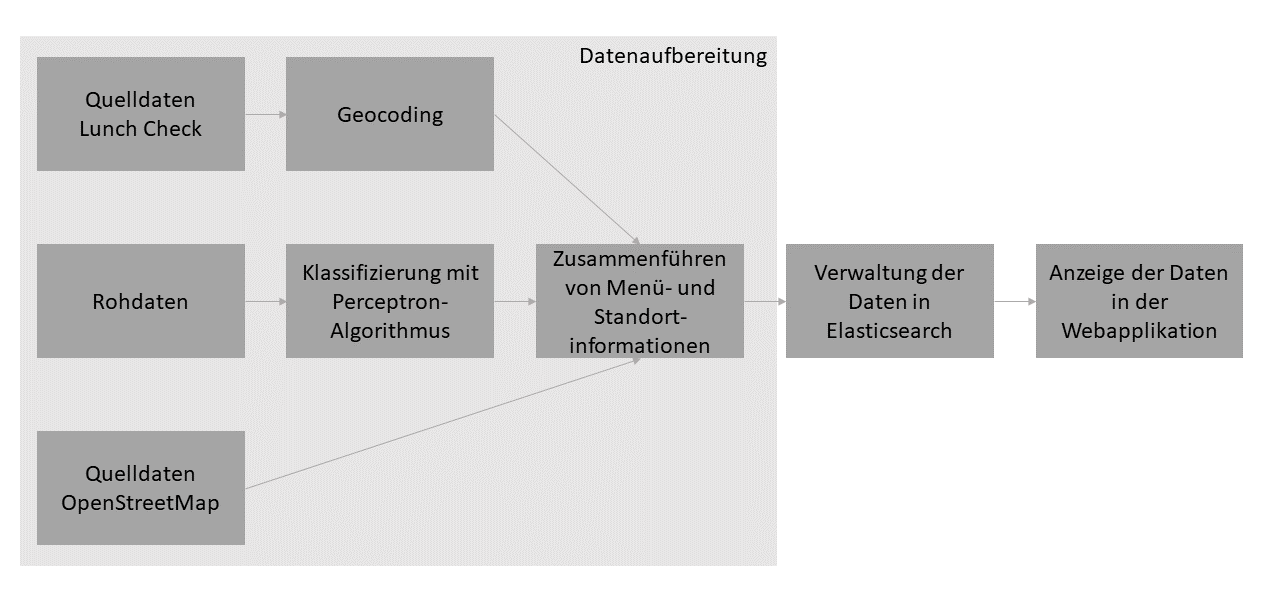
\includegraphics[width=1\columnwidth,keepaspectratio]{img/Ablauf_prod_pipeline.png}
	\caption{Produktive Pipeline mit Datenaufbereitung}
	\source{Eigene Darstellung}
	\label{fig:prod_pipeline}
\end{figure}
Diese hat das Ziel, die Rohdaten zu klassifizieren und die als Menüseiten klassifizierten Webpages mit Informationen bezüglich des Standorts zu versehen.
Es ist der trainierte Machine-Learning-Algorithmus \glqq Perceptron mit binärem Bag of Words\grqq{} eingesetzt worden, um die Rohdaten des Webcrawlers zu klassifizieren.
Um die als Menüseiten klassifizierten Webpages mit Geoinformationen zu versehen, wurden die ursprünglichen Daten von Openstreetmap und Lunch Check verwendet. Dies aus dem Grund, da die Daten von OpenStreetMap bereits die Koordinaten des Restaurants beinhalteten.
Die Daten von Lunch-Check waren nicht mit Geoinformationen versehen, jedoch mit den Adressinformationen.
Diese wurden genutzt, um  die Daten mittels Geocoding, genauer mit einer lokalen Installation von Nominatim\footnote{\url{https://nominatim.openstreetmap.org/}abgerufen am: 02.07.2019} mit den Geoinformationen zu erweitern.
Über den Host-Anteil der URL wurden die Menüseiten den Restaurants zugeordnet.
Somit ist aus mehreren Quellen eine einheitliche Datenstruktur im JSON-Format erstellt worden.
Diese Struktur wird in \cref{fig:json_struktur} verdeutlicht.
\begin{figure}[H]
	\centering
	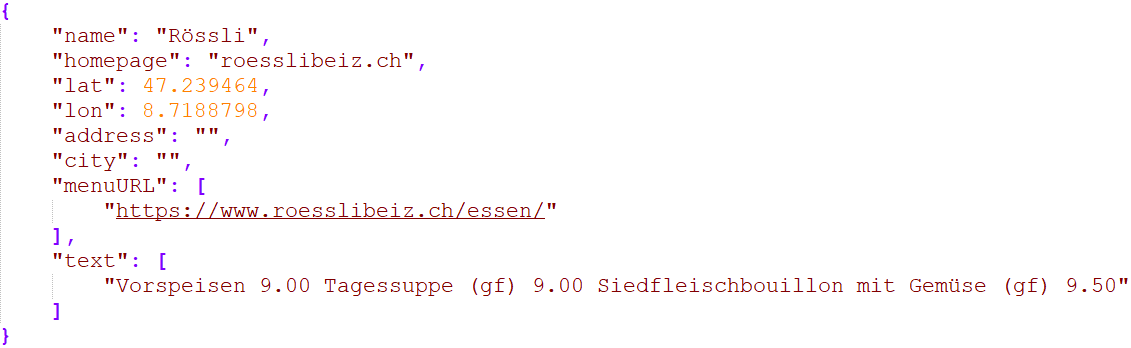
\includegraphics[width=1\columnwidth,keepaspectratio]{img/json_struktur.png}
	\caption{JSON-Struktur anhand eines Beispiels(Anmerkung: Der Text wurde manuell gekürzt)}
	\source{Eingene Darstellung}
	\label{fig:json_struktur}
\end{figure}
Der Link zum Code dieser Standardisierung der Daten ist im Anhang unter \cref{app:prodpipeline} zu finden.
\FloatBarrier
\subsection{Idee}
Ziel der Webapplikation ist es, dass ein Benutzer einfach und überschaubar nach Menüs suchen kann.
Um dies zu erreichen, wurde ein Mockup mit dem Layout der Benutzeroberfläche erstellt, welches in \cref{fig:webapp_mockup} dargestellt wird.
\begin{figure}[H]
	\centering
	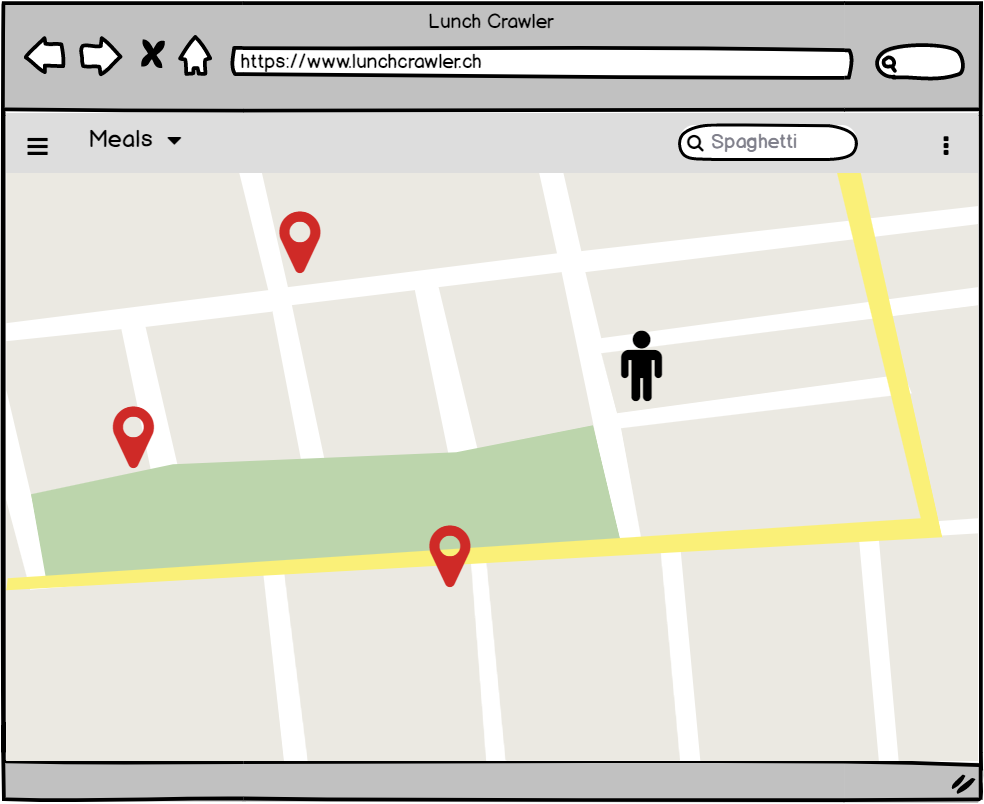
\includegraphics[width=0.7\columnwidth,keepaspectratio]{img/webapp_mockup.png}
	\caption{Mockup der Webapplikation}
	\source{Eigene Darstellung}
	\label{fig:webapp_mockup}
\end{figure}
Dieses enthält lediglich eine Kartenansicht und einen Suchbalken.
Der Standort des Benutzers soll beim Aufruf der Webapplikation abgefragt werden, damit der Kartenfokus auf diesen gesetzt werden kann.
Durch die Eingabe einer Speise im Suchbalken werden alle Restaurants angezeigt, welche diese Speise in ihrer Menükarte aufführen.
\subsection{Frontend}
Das Frontend ist nach dem Prinzip einer Single-Page-Applikation aufgebaut.
Eine HTML-Datei dient als Grundgerüst und wird durch die entsprechenden JavaScript-Dateien angepasst.
Um ein ansprechendes Layout und Responsive Design zu gewährleisten, wird die Bibliothek \glqq Bootstrap\footnote{\url{https://getbootstrap.com/} abgerufen am: 17.07.2019}\grqq{} verwendet.
Durch die Geolocation API\footnote{\url{https://www.w3schools.com/html/html5_geolocation.asp} abgerufen am: 17.07.2019} wird der Standort des Benutzers abgefragt.
Das Verwenden des Suchbalkens löst eine Fetch-Anfrage auf das Backend aus.
Die Ergebnisse dieser Anfrage werden dann mit der Bibliothek \glqq Leaflet\footnote{\url{https://leafletjs.com/} abgerufen am: 17.07.2019}\grqq{} angezeigt.
Für jedes Restaurant wird ein Marker mit einem Popup-Fenster erstellt, welches einen Link zur Homepage sowie der Menüseite beinhaltet.
\subsection{Backend}
Als serverseitige Plattform wird \glqq Node.js\footnote{\url{https://nodejs.org/} abgerufen am: 17.07.2019}\grqq{} verwendet, da bereits Erfahrung mit dieser Technologie gemacht wurde und sie für Fast Prototyping geeignet ist.
Ein Aufruf der Basis-URL stellt die HTML-Datei sowie die entsprechenden JavaScript-Dateien des Frontends zur Verfügung.
Das Verwenden des Suchbalkens gibt die Informationen über den Standort sowie das Such-Query an das Backend weiter.
Dieses löst eine Fetch-Anfrage auf das Search Engine aus, welche die entsprechenden Resultate als JSON zurückliefert.
Diese JSON-Dateien werden dann an das Frontend weitergeleitet.
\subsection{Search Engine}

Das Search Engine dient in diesem Fall dazu, die Daten der produktiven Pipeline zu verwalten und diese der Webapplikation zur Verfügung zu stellen.
Somit übernimmt sie die Funktionalität einer Datenbank, mit dem Vorteil, dass die Daten schneller suchbar sind.
Als Search Engine wird die Software \glqq Elasticsearch\grqq{} eingesetzt\footnote{\url{https://www.elastic.co/de/products/elasticsearch} abgerufen am: 07.05.2019}.
Da StormCrawler SDK entsprechende Komponenten zur Anbindung anbietet\footnote{\url{http://stormcrawler.net/getting-started/} abgerufen am: 07.05.2019} und dies in Betracht gezogen wurde, wird diese Software eingesetzt.
Elasticsearch wird in einem Docker-Container betrieben\footnote{\url{https://www.elastic.co/guide/en/elasticsearch/reference/current/docker.html} abgerufen am: 07.05.2019}.
Daten können im JSON-Format mittels HTTP-Request (POST) darin abgelegt werden\footnote{\url{https://www.elastic.co/guide/en/elasticsearch/reference/current/docs-index_.html} abgerufen am: 07.05.2019}.
Ebenfalls mittels HTTP-Request (GET) können Suchabfragen auf die darin enthaltenen Daten getätigt werden\footnote{\url{https://www.elastic.co/guide/en/elasticsearch/reference/6.4/search-search.html} abgerufen am: 07.05.2019}.
\subsection{Benutzung der Webapplikation}
Die Webapplikation ist erst ein Prototyp.
Da das Deployment der Search Engine kostenpflichtig ist, wurde von einem Deployment abgesehen.
Um die Webapplikation trotzdem benutzen zu können, folgt nun eine Anleitung.\\

Voraussetzungen
\begin{itemize}
	\item Docker
	\item Node.js
	\item npm
	\item Webbrowser (getestet mit Mozilla Firefox)
\end{itemize}
Ablauf der Installation
\begin{enumerate}
	\item Das Github-Repository \url{https://github.com/s-santoro/lunch-crawler} herunterladen
	\item Docker-Image von Elasticsearch herunterladen:\\
	docker pull docker.elastic.co/elasticsearch/elasticsearch:7.0.1
	\item Docker-Container starten:\\
	docker run -p 9200:9200 -p 9300:9300 -e "discovery.type=single-node" \\ docker.elastic.co/elasticsearch/elasticsearch:7.0.1
	\item Das Zipfile \glqq/lunch-crawler/webapp-lunch-crawler/run\textunderscore webapp/data\textunderscore for\textunderscore elasticSearch.zip\grqq{} entpacken
	\item Das Script \glqq/lunch-crawler/webapp-lunch-crawler/run\textunderscore webapp/add\textunderscore to\textunderscore elasticsearch.sh\grqq{} ausführen
	\item In den Ordner \glqq/lunch-crawler/webapp-lunch-crawler\grqq{} wechseln
	\item Den folgenden Befehl ausführen: npm init
	\item Den folgenden Befehl ausführen: npm install
	\item Den folgenden Befehl ausführen: npm start
\end{enumerate}
Benutzung der Webapplikation
\begin{enumerate}
	\item Gewünschtes Gericht im Suchfeld eingeben
	\item Standortabfrage zulassen
	\item Ergebnisse betrachten (falls kein Ergebnis angezeigt wird, muss manuell herausgezoomt werden)
\end{enumerate}

\newpage

\chapter{Fazit}
In diesem Teil werden Erkennisse der jeweiligen Bereiche aufgeführt.
Diese wurden während der Arbeit erkannt und als wichtig angesehen.
\section{Webcrawler}
Eine Evaluation des Webcrawlers wäre von Vorteil gewesen.
StormCrawler hat zwar die Funktion erfüllt, dieser ist jedoch dafür ausgelegt, eine enorme Masse an Websites und Webpages zu crawlen.
Dies ist jedoch keine Hauptanforderung in dieser Arbeit gewesen.
Dafür wäre ein Webcrawler, welcher auch dynamisch generierte Websites handhaben kann, von Vorteil gewesen.
\section{Klassifizierung}
Für die Klassifizierung hätte eine Preprocessing-Methode zur Erkennung des Hauptinhalts einer Webpage einen grossen Benefit bewirkt.
Beim manuellen Labeling wurde erkannt, dass viele Webpages nicht relevante oder sogar irreführende Informationen im Kopf- und Fussteil beinhalten.
Der Gold Standard sollte ein zweites Mal gelabelt werden, damit dieser nach dem Vier-Augen-Prinzip kontrolliert werden würde.
Von diesem Schritt wurde jedoch aus zeitlichen Gründen abgesehen.
Um die regelbasierte Klassifikation zu verbessern, wären komplett neue Regeln sowie das erweitern und anpassen der Listen wertvoll.
\newpage

\chapter{Selbstständigkeitserklärung}
\label{sec:erklaerung}
\vspace{0 cm}
Wir erklären hiermit, dass wir die vorliegende Arbeit selbstständig und ohne fremde Hilfe verfasst und keine anderen Hilfsmittel als angegeben verwendet haben. Insbesondere versichern wir, dass wir alle wörtlichen und sinngemässen Übernahmen aus anderen Werken als solche kenntlich gemacht haben.
\\
\\
Name: Sandro Santoro
\\	
Ort, Datum: \hspace{4cm}Unterschrift:
\\
\\
\\
Name: Gian Brunner
\\
Ort, Datum: \hspace{4cm}Unterschrift:
\\
\\





\newpage

%Literaturverzeichnis
\bibliographystyle{apacite}
\bibliography{bibfile}

%Verzeichnis aller Tabellen
\listoftables

%Verzeichnis aller Bilder
\listoffigures

\chapter{Anhang}
\section{Elektronischer Anhang}
\begin{itemize}
	\item Quelldatei OpenStreetMap für Seed (JSON-Datei)
	\item Quelldatei Lunch Check für Seed (Excel-Datei)
	\item Schlussendliches Seedfile (txt-Datei)
	\item Klassifikationsdatei (Pickle-Datei)
\end{itemize}
\section{Verlinkungen}
\subsection{Webcrawler}
\begin{itemize}
	\item Implementierung StormCrawler\\ \url{https://github.com/s-santoro/lunch-crawler/tree/master/storm-crawler-master}
	\item Angepasste Kompontenten\\
	\url{https://github.com/s-santoro/lunch-crawler/tree/master/storm-crawler-master/archetype/src/main/resources/archetype-resources/src/main/java/ntb/iks}
	\item Docker-Compose\\
	\url{https://github.com/s-santoro/lunch-crawler/tree/master/storm-cluster}
	\item Script zur Analyse der gecrawlten Rohdaten\\
	\url{https://github.com/s-santoro/lunch-crawler/blob/master/storm-crawler-master/scripts/website_histogram.py}
\end{itemize} 
\subsection{Gold Standard}
\label{app:gold_standard}
\begin{itemize}
	\item Gold Standard\\ 
	\url{https://github.com/s-santoro/lunch-crawler/blob/master/gold-standard/Gold_Standard.zip}
	\item Tool zum manuellen Labeln\\ 
	\url{https://github.com/s-santoro/lunch-crawler/tree/master/gold-standard/labeling_tool}
	\item Script zur Extrahierung zufälliger Daten aus den gecrawlten Rohdaten\\ 
	\url{https://github.com/s-santoro/lunch-crawler/blob/master/gold-standard/generate_randomfiles.sh}
\end{itemize} 
\subsection{Klassifikationspipeline}
\label{app:classification}
\begin{itemize}
	\item Datenimport\\ 
	\url{https://github.com/s-santoro/lunch-crawler/blob/master/classification/scripts/Importer.py}
	\item Preprocessing\\ 
	\url{https://github.com/s-santoro/lunch-crawler/blob/master/classification/scripts/Preprocessor.py}
	\item Regelbasierte Klassifikation\\ 
	\url{https://github.com/s-santoro/lunch-crawler/blob/master/classification/scripts/RulebasedClassifier.py}
	\item Klassifikation mittels Machine Learning\\ 
	\url{https://github.com/s-santoro/lunch-crawler/blob/master/classification/scripts/MLClassifiers.py}
	\item Evaluierung der Klassifikation\\ 
	\url{https://github.com/s-santoro/lunch-crawler/blob/master/classification/scripts/Evaluator.py}
	\item Visualisierung der Klassifikation\\ 
	\url{https://github.com/s-santoro/lunch-crawler/blob/master/classification/scripts/DataVisualizer.py}
	\item Konfiguration für regelbasierte Klassifikation\\ 
	\url{https://github.com/s-santoro/lunch-crawler/blob/master/classification/scripts/configs/ConfigurationsRB.py}
	\item Konfiguration für Klassifikation mittels Machine Learning\\ 
	\url{https://github.com/s-santoro/lunch-crawler/blob/master/classification/scripts/configs/ConfigurationsML.py}
	\item Stoppwortliste\\ 
	\url{https://github.com/s-santoro/lunch-crawler/blob/master/classification/stopwords_no_umlaute.txt}
	\item Getränkeliste\\ 
	\url{https://github.com/s-santoro/lunch-crawler/blob/master/classification/beverage_list.txt}
	\item Blacklist\\ 
	\url{https://github.com/s-santoro/lunch-crawler/blob/master/classification/blacklist.txt}
	\item Whitelist\\ 
	\url{https://github.com/s-santoro/lunch-crawler/blob/master/classification/whitelist.txt}
\end{itemize} 
\subsection{Produktive Pipeline}
\begin{itemize}
	\item Pipeline zur Klassifikation der Rohdaten\\ 
	\url{https://github.com/s-santoro/lunch-crawler/tree/master/prod-pipeline/classification}
	\item Script zur Standardisierung von Restaurantinformationen\\ 
	\url{https://github.com/s-santoro/lunch-crawler/blob/master/prod-pipeline/nodejs/standardize_data.js}
	\item Script zur Analyse von Restaurantinformationen\\ 
	\url{https://github.com/s-santoro/lunch-crawler/blob/master/prod-pipeline/nodejs/analyze_data.js}
\end{itemize} 




\end{document}
